\errorcontextlines32
\documentclass[11pt]{book} %twoside and openright are default for the the book class
\title{Title}
\author{Carla Filosa}
\date{\today}

\usepackage{cmtt,lmodern}      %Computer Modern Bright text with Latin Modern math
\usepackage[T1]{fontenc}           %T1 font encoding to copy and search symbols like
\usepackage[UKenglish,dutch]{babel} %for appropriate hyphenation


\usepackage[paperwidth=17cm,paperheight=24.5cm,top=2.51cm,bottom=2.005cm,inner=2.5cm,outer=1.5cm,headheight=12.0pt,headsep=0.58cm]{geometry}



%!TEX root = thesis.tex
%%%% PACKAGES %%%%
\usepackage[T1]{fontenc}
%\usepackage[utf8]{inputenc}
\usepackage{amsmath,amsfonts,amssymb,amsthm}
\usepackage{mathrsfs}
\usepackage{mathtools}
\usepackage{dsfont}
\usepackage[hidelinks]{hyperref}  %to adapt page numbers in pdf. The option [hidelinks] hides hyperlinks
\usepackage{color}            %for nb comments
\usepackage{setspace}
%Figures
\usepackage{wrapfig}
\usepackage{float}
\usepackage{subcaption}
\usepackage{longtable}
\usepackage{multirow}
%\usepackage{acro}
%\addtolength{\subfigcapskip}{-25pt}
%\addtolength{\subfigbottomskip}{-25pt}
%\addtolength{\subfigtopskip}{-25pt}
%Watermark
%\usepackage{draftwatermark}
%\SetWatermarkText{DRAFT}
%\SetWatermarkScale{1}

\usepackage{algorithm}
\usepackage{algpseudocode}
%\usepackage[notcite,notref]{showkeys}

\usepackage{enumitem}% http://ctan.org/pkg/enumitem
%\setlist{nolistsep}
%\setlist[enumerate]{topsep=0pt}
\usepackage{epstopdf}
\usepackage{graphicx}
%\usepackage{biblatex}
%\usepackage{fullpage}
\usepackage{mathtools}
\usepackage{nomencl}
\usepackage{verbatim}
\usepackage{tikz}
\usetikzlibrary{shapes,arrows}
\usepackage{textcomp}         %for copyright symbol and bullets
\usepackage[nottoc]{tocbibind} %include bibliography in toc (don't put the toc itself in the toc)
\usepackage{url}              %for url's in bibliography

%\setlength{\parindent}{0pt}
%\setlength{\parskip}{\baselineskip}

%TOC
\usepackage[titles]{tocloft}
%\setlength\cftparskip{-5pt}
%\setlength\cftbeforesecskip{-5pt}
%\setlength\cftaftertoctitleskip{0.5pt}
\setlength\cftparskip{-2pt}
\setlength\cftbeforesecskip{1pt}
\setlength\cftaftertoctitleskip{2pt}
%Footnote without number
\newcommand\blfootnote[1]{%
  \begingroup
  \renewcommand\thefootnote{}\footnote{#1}%
  \addtocounter{footnote}{-1}%
  \endgroup
}

\usepackage{afterpage}

\newcommand\blankpage{%
    \null
    \thispagestyle{empty}%
    \addtocounter{page}{-1}%
    \newpage}

%%%%% THEOREMS, etc ... %%%%%%%

\theoremstyle{plain}
\newtheorem{theorem}{Theorem}[section]
\newtheorem{thm}[theorem]{Theorem}
\newtheorem{lemma}[theorem]{Lemma}
\newtheorem{lem}[theorem]{Lemma}
\newtheorem{prop}[theorem]{Proposition}
\newtheorem{corollary}[theorem]{Corollary}
\newtheorem{cor}[theorem]{Corollary}
\newtheorem{hyp}[theorem]{Hypothesis}
\newtheorem{defn}[theorem]{Definition}
\newtheorem{definition}[theorem]{Definition}
\theoremstyle{definition}
\newtheorem{assume}[theorem]{Assumption}

\theoremstyle{remark}
\newtheorem{example}[theorem]{Example}
\newtheorem{ex}[theorem]{Example}
\newtheorem{remark}[theorem]{Remark}
\newtheorem{rem}[theorem]{Remark}
\newtheorem{nota}[theorem]{Notation}
\numberwithin{equation}{section}
\newtheorem*{theorem*}{Theorem}

%%%%%%%%%%%%%%%BRS%%%%%%
\newcommand{\R}{\mathbb{R}}

%%%%%COLORS%%%%%%%%

\newcommand{\US}{\color{red}}


\newcommand\skp[2]{\left\langle #1 , #2 \right\rangle}
\newcommand\bra[1]{\left({#1}\right)}
\newcommand\pra[1]{\left[{#1}\right]}

%\newcommand\set[1]{\left\{#1\right\}}
\newcommand\norm[1]{\left\lVert#1\right\rVert}
\newcommand\abs[1]{\left\lvert#1\right\rvert}
\DeclareMathOperator*{\argmax}{arg\,max}
\DeclareMathOperator*{\argmin}{arg\,min}
\DeclareMathOperator*{\esssup}{ess\,sup}
\DeclareMathOperator{\variable}{var}
\DeclareMathOperator{\Id}{Id}
\DeclareMathOperator{\Jac}{Jac}
\DeclareMathOperator{\J}{J}
\DeclareMathOperator{\Tr}{tr}
\DeclareMathOperator{\AC}{AC}
\DeclareMathOperator{\PI}{PI}
\DeclareMathOperator{\TI}{TI}
\DeclareMathOperator{\LSI}{LSI}
\newcommand{\EX}[1][E]{\ensuremath {\mathds{#1}}}





\def\div{\mathop{\mathrm{div}}\nolimits}
\def\US{\color{red}}
\def\vep{\varepsilon}
\DeclareMathOperator{\TV}{TV}



% Definition of undecided symbols
%\DeclareMathOperator{\RelEnt}{H}
\def\RelEnt{\mathbf H}
%\DeclareMathOperator{\RF}{RF}
\def\RF{\mathbf{RF}}
\DeclareMathOperator{\Wasser}{W}
\DeclareMathOperator{\I}{I}
\def\I{\mathbf{I}}
\def\Hausdorff{\mathcal{H}}





%%%%%%From DOG paper%%%%%
\def\opN{\mathcal N}
\def\LDJ{\mathcal J}
\def\hrho{\hat{\rho}}
\def\opL{\mathscr L}
\DeclareMathOperator\Int{Int}
\def\Lebesgue{\mathcal L}
\def\g{\gamma}
\def\G{\Gamma}
\newcommand\TA{T\!A}
\def\d{\delta}

\DeclareMathOperator{\supp}{supp}


\makeatletter
\newenvironment{largefigure}[1][0pt]{ 
  \clearpage % finish last page and flush previous floats
  % save current textheight
  \newlength{\@prevtextheight}\setlength{\@prevtextheight}{\textheight} 
  % extend textheight and recompute internal float parameters
  \setlength{\textheight}{\textheight + #1}
  \global\@colht\textheight % reset \@colht 
  \global\@colroom\textheight % reset \@colroom
  \@floatplacement
  % force float to appear at top of page
  \setlength{\@fptop}{0pt} 
  \begin{figure}[!p]
}{
  \end{figure}
  \clearpage % flush the float
  % restore textheight and all
  \setlength{\textheight}{\@prevtextheight}
  \global\@colht\textheight 
  \global\@colroom\textheight
  \@floatplacement
  \setlength{\@fptop}{0pt plus 1fill}
}
\makeatother




%% end code


\graphicspath{{figures/}}
\newenvironment{dedication}
  {\clearpage           % we want a new page
   \thispagestyle{empty}% no header and footer
   \vspace*{\stretch{1}}% some space at the top 
   \itshape             % the text is in italics
   \raggedleft          % flush to the right margin
  }
  {\par % end the paragraph
   \vspace{\stretch{3}} % space at bottom is three times that at the top
   \clearpage           % finish off the page
  }
%\usepackage{titlesec}
%\titleformat{\section}{\newpage \large\bfseries}
%{\thesection.}{0.5em}{} 
%
%\titlespacing{\section}{12pc}{1.5ex plus .1ex minus .2ex}{1pc}
%\usepackage[backend=biber,style=alphabetic,citestyle=authoryear]{biblatex}
\usepackage[backend=biber,style=authoryear,]{biblatex}
\addbibresource{BIB1.bib}
\usepackage{fancyhdr}
\usepackage{appendix} % For appendix
\usepackage[utf8]{inputenc}


\begin{document}
\mbox{}

%\begin{spacing}{1.1}

\pagenumbering{gobble}  %geen paginanummers
%\selectlanguage{UKenglish}

\selectlanguage{UKenglish}

\thispagestyle{plain}

\vspace*{4cm}

\begin{center}
{\Huge \textbf{TITLE}}\\
\vspace{1cm}
{\huge{Carla Filosa}}
\end{center}



\clearpage
\thispagestyle{plain}

\vspace*{\fill}



%\noindent Cover picture: Target phase space of a parabolic reflector. \\
%Cover design by Carlo Lancia 

%\vspace{1cm}

%\noindent A catalogue record is available from the Eindhoven University of Technology Library\\
%\\
%\noindent ISBN:  978-90-386-4504-9\\

\vspace{1cm}

\noindent Copyright \copyright{} 2019 by C. Filosa. \\
All rights are reserved. No part of this publication may be reproduced, stored in a retrieval system, or transmitted, in any form or by any means, electronic, mechanical, photocopying, recording or otherwise, without prior permission of the author.

\clearpage

\selectlanguage{dutch}

\thispagestyle{plain}

\begin{center}
\begin{large}
\vspace*{3cm}
\textbf{title}

\vspace*{2cm}

%PROEFSCHRIFT

\vspace*{1.5cm}

%ter verkrijging van de graad van doctor aan de \\ Technische Universiteit Eindhoven, op gezag van de \\ rector magnificus prof.dr.ir. F.P.T. Baaijens, voor een \\ commissie aangewezen door het College voor \\ Promoties, in het openbaar te verdedigen \\  op woensdag 30 mei 2018 om 16:00 uur 






\vspace*{1.5cm}

%door

\vspace*{1.5cm}

Carla Filosa

\vspace*{1.5cm}

%geboren te Torre del greco, Itali\"e 

\end{large}
\end{center}

%\clearpage
%\thispagestyle{plain}
%\begin{large}
%\noindent Dit proefschrift is goedgekeurd door de promotoren en de samenstelling van de promotiecommissie is als volgt:\\
%\vspace{0.4cm}\\
%\begin{tabular}{ll}
%voorzitter: & prof.dr. \\
%$1^{\text{e}}$ promotor: & prof.dr. W.L. IJzerman \\
%copromotor: &  dr. J.H.M. ten Thije Boonkkamp \\
%leden: % &  prof.dr.  \\
%&  prof.dr.\\
 %&  \\
 %&  prof.dr.  \\
 %&  dr.i \\
%\end{tabular}

%\vspace*{10cm}
%\noindent Het onderzoek of ontwerp dat in dit proefschrift  wordt beschreven is uitgevoerd in overeenstemming met de TU/e Gedragscode Wetenschapsbeoefening.
%\end{large}
%\clearpage

\selectlanguage{UKenglish}



\pagenumbering{roman}


%\chapter*{}
%\pagenumbering{gobble}
%\renewcommand{\epigraphwidth}{\setlength{12cm}}
\clearpage{\pagestyle{empty}\cleardoublepage}
%\begin{center}
%{\Large  ``{ To  \\[2\baselineskip] }''}
%\end{center}

%\renewcommand{\epigraphwidth}{\setlength{5cm}}


%\include{chapters/abstract}

%\clearpage{\pagestyle{empty}\cleardoublepage}


\pagestyle{empty}

\setcounter{tocdepth}{1}
\tableofcontents


\clearpage{\pagestyle{empty}\cleardoublepage}


%%%%%FANCYHDR%%%%%%%%%%%%%

\pagestyle{fancy}


\renewcommand{\chaptermark}[1]{ \markboth{#1}{}}

\renewcommand{\sectionmark}[1]{}



%%%%%%%%%

\pagenumbering{arabic}


%%%%%Chapters%%%%%
%%%%\chapter{Exact intensity for the two-faceted cup}\label{app:boundariescup}
For very simple optical systems, the \textit{exact} target intensity of light can be calculated. Here we explain how this is done for the two-faceted cup with a Lambertian source described in Chapter \ref{chap:raytracing}. We remind the reader that, for this system, the intensity in a given direction $\variabile{p}$ in PS is defined as:
\begin{equation}\label{eq:eta_appendix}
I_{\textrm{PS}}(\variabile{p}) = \sum_{\Pi}\int_{\variabile{q}^\textrm{\,min}(\Pi, \variabile{p})}^{\variabile{q}^\textrm{\,max}(\Pi,\variabile{p})}L(\variabile{q}, \variabile{p})\textrm{d}\variabile{q} = \sum_{\Pi}\big (\variabile{q}^\textrm{max}(\Pi,\variabile{p})-\variabile{q}^\textrm{\,min}(\Pi,\variabile{p})\big )\,,
\end{equation}
where the sum is over all the possible paths, $\variabile{q}^\textrm{\,min}(\Pi,\variabile{p})$ and $\variabile{q}^\textrm{\,max}(\Pi,\variabile{p})$ are of the intersection points between the line $\variabile{p}=\textrm{const}$ and $\partial$\insieme{R}$_\textrm{t}(\Pi)$, and the second equation holds as we assume $L=1$ in \insieme{R}$_\textrm{t}(\Pi)$.
Therefore, if we are able to provide an analytic expression for the boundaries $\partial$\insieme{R}$_\textrm{t}(\Pi)$ we can calculated the position coordinates $\variabile{q}^\textrm{\,min}(\Pi,\variabile{p})$ and $\variabile{q}^\textrm{\,max}(\Pi,\variabile{p})$ analytically and we can compute the exact intensity for every direction $\variabile{p}$ is obtained using (\ref{eq:eta_appendix}). The procedure used for such purpose is explained next.
\section{Analytic approach}
The idea is to rotate the cup to determine the maximum number of reflections between a ray and the optical lines before reaching the target. The rays are considered to be straight lines instead of broken lines. Hence it is sufficient to find only one intersection point between the ray and a line segment (also in the case where more than one reflection occurs). Finally transforming (rotating or reflecting) back these points we obtain the corresponding coordinates at the target.\\ \indent
The two-faceted cup is defined in the $(\variabile{x}, \variabile{z})$-plane as in Chapter \ref{chap:raytracing}. 
Let $\gamma\in(0, \pi/2)$ be the angle that the left and right reflector make with the normal to the source. 
%\begin{figure}[t]
%\label{fig:cup}
%  \begin{center}
%%\vspace{-1.5cm}
%  \includegraphics[width=6.7cm]{cup.pdf}
%  \end{center}
%%\vspace{-2cm}
%  \caption{\textbf{Shape of the two-faceted cup.}  Each line of the system is labeled with a number.
%   The source \point{S}$= [-2,2]$ (line number $1$) is located on the $\variabile{x}$-axis.
%   The target \point{T}$= [-17, 17]$ (line $4$) is parallel to the source and is located at a height $\variabile{z}= 40$.
%   The left and right reflectors (line $2$ and $3$) connect the source with the target.}
%  \label{fig:cup}
%\end{figure}
The maximum $\variabile{z}$-coordinate that the two-faceted cup can reach during the rotation is defined by the $\variabile{z}$-coordinate of the point $\point{P}=(0,Z)$:
\begin{equation}\label{rotation}\begin{tabular}{llll}
$Z$ & $=$ & $ \big(h+\frac{\variabile{a}}{\tan\gamma}\big)\frac{1}{\cos\gamma}-\frac{\variabile{a}}{\tan\gamma}$ \\ $ \quad$ & $ \quad $ & $ \quad $ \\$ \quad$ &  $=$ & $\frac{h}{\cos\gamma}+\frac{\variabile{a}(1-\cos\gamma)}{\sin\gamma},$\end{tabular}
\end{equation} and $\point{R}=(0,-\frac{\variabile{a}}{\tan\gamma})$ is the rotation point. We define $\point{B}_k$ as the clockwise ($k<0$) or counterclockwise ($k\geq 0$) rotation image of $\point{P}$ around the point $\point{R}$ over an angle $\alpha_k=(2k+1)\gamma$, with $k$ an integer number (Figure \ref{fig:twofaced} is illustrative).
\begin{figure}[t]%\label{fig:twofaced}
 \centering
  \includegraphics[width=\textwidth]{rotated_cup.pdf}
 \caption{\textbf{The two-faceted cup rotated twice on both sides.} The line segment with end points $B_{k-1}$ and $B_{k}$ is the $|k|$ times rotated target. The coordinates $(q,h)$ on the target $B_{-1}B_{0}$ are obtained by transforming the coordinates $(u,v)$ of the intersection point between a ray and the segment $B_0B_1$ . The point $\point{R} = \big(0,-\frac{a}{\tan{\gamma}}\big)$ is the center of the circle described by rotating the cup (dashed line).}
  \label{fig:twofaced}
  \end{figure}
  %as the notation used in equation ($\ref{Bk}$) could suggest.
The position coordinates of points $\point{B}_k = (B_{k,x}, B_{k,z})$ are given by:
\begin{equation}
 \begin{pmatrix} B_{k,x}  \\  B_{k,z}\end{pmatrix}= -
  \begin{pmatrix} 0  \\  \frac{a}{\tan\gamma}\end{pmatrix}+
 \left(\begin{split}  & \cos\alpha_k  & -\sin\alpha_k \\  & \sin\alpha_k & \cos\alpha_k\end{split}\right).
 \begin{pmatrix}  0 \\  Z+\frac{a}{\tan\gamma}\end{pmatrix},
\end{equation}
The maximum number of reflections $r_{\textrm{max}}$ a ray can undergo before arriving at the target is:
\begin{equation}
r_{\textrm{max}}=\max\{k\in\mathbb{N} \;| \; B_{k-1,z}\geq 0\}.
\end{equation}
For example, for the two-faceted cup depicted in Figure \ref{fig:cup}, we found $r_{\textrm{max}}=2$.\\ \indent 
Given the coordinates $(\variabile{x}_1, \variabile{z}_1)$ and the angular coordinate $\optangle_1$ of a ray at the source, we can calculate the corresponding position $(\variabile{x}, \variabile{z})$ and direction coordinate $\optangle$ at the target as explained in the following. \\ \indent We compute the coordinates $(u,v)$ of the intersection point between the ray parametrization and the $|\variabile{k}|$ times rotated or reflected target $\point{B}_{\variabile{k}-1}\point{B}_\variabile{k}$ for which the intersection with the forward ray is not empty, for $\variabile{k}=-\variabile{r}_{\textrm{max}}-1, \cdots, \variabile{r}_{\textrm{max}}$. Next, if $\variabile{k}$ is even, the corresponding coordinates $(\variabile{x},\variabile{z})$ at the target are found by rotating back the coordinates $(\variabile{u},\variabile{v})$, otherwise a reflection is applied. Therefore, the ray coordinates $(\variabile{x},\variabile{z})$ at the target are given by:
\begin{equation} \label{rotation_target}\begin{pmatrix} \variabile{x}\\ \variabile{z}
\end{pmatrix} = \left(\begin{array}{cc}(-1)^k & 0  \\ 0 & 1\end{array}\right)
\left(\begin{array}{cc}\cos(-2\variabile{k}\gamma) & -\sin(-2\variabile{k}\gamma) \\\sin(-2\variabile{k}\gamma) & \cos(-2\variabile{k}\gamma)\end{array}\right)\begin{pmatrix} \variabile{u} \\
 \variabile{v}+\frac{a}{\tan(\gamma)}\end{pmatrix}-\begin{pmatrix}0 \\ \frac{a}{\tan\gamma}\end{pmatrix}.
\end{equation} We observe that the sign in the first matrix depends on the parity of $\variabile{k}$. When $\variabile{k}=0$, i.e., the ray does not reflect, the first matrices become the identity matrix and the cup is not rotated nor reflected. When $\variabile{k}$ is even, the determinant of the matrix given by the product between the first and the second matrix (\ref{rotation_target}) is equal to $1$ and we obtained a rotation matrix, while when $\variabile{k}$ is odd the determinant of the product matrix is $-1$ and we have a reflection matrix.
\\ \indent
The method of transforming the cup instead of the rays allows us to determine the positive luminance regions $\mbox{\insieme{R}}_1(\Pi_{\variabile{j}})$ and $\mbox{\insieme{R}}(\Pi_{\variabile{j}})$ in source and target PS, where every path $(\Pi_{\variabile{j}})_{\variabile{j}=1, \cdots, 2\variabile{r}_{\textrm{max}}+1}$ corresponds to $|\variabile{k}|$ reflections. The corresponding boundaries only consist of rays that either leave the extremes of the source or hit one of the points $\point{B}_\variabile{k}$. 
%At the boundaries a small change in the position or direction ray coordinate can cause a difference in the number of the reflections. 


Rays that leave the interior of \point{S} and hit $\point{B}_\variabile{k}$ have as position coordinates in source PS $\variabile{q}_1 = \variabile{x}_1\in(-\variabile{a}, \variabile{a})$, the corresponding target PS coordinates are $\variabile{q} = \variabile{x} = B_{\variabile{k}, \variabile{x}}$.
The direction coordinates of these rays at the source PS are $\variabile{p}_1 = \sin(\optangle_1)$ where $\optangle_1$ is given by:
\begin{equation}\label{anglesource}
\optangle_1 = \arctan\bigg(\frac{\variabile{x}_1-B_{k,x}}{B_{k,z}}\bigg).
\end{equation}
The corresponding direction coordinates at the target PS are $\variabile{p}=\sin(\optangle)$ where $\optangle$ is given by:
\begin{equation}\label{teta}
\optangle=(-1)^\variabile{k}(\optangle_1-2\variabile{k}\gamma).
\end{equation}

Rays emitted from the end points of the source have a constant position coordinate $\variabile{q}_1 = \variabile{x}_1 = \textrm{const}$ in source PS and varying a direction coordinate $\variabile{p}_1 = \sin(\optangle_1)\in[-1, 1]$ where $\optangle_1\in[-\pi/2, \pi/2]$. The corresponding target position coordinate $\variabile{x}$ is obtained from (\ref{rotation_target}) while the direction coordinate in the target PS is $\variabile{p} = \sin(\optangle)$, where $\optangle$ is given by Equation (\ref{teta}).
Note that the rays emitted from the end points of the source form vertical lines in source PS as $\variabile{q}_1= \textrm{const}$ and $\variabile{p}_1\in[-1,1]$ varies.
On the other hand, rays that hit points $\point{B}_k$ form vertical lines in target PS as $\variabile{q} = \textrm{const}$.
\\ \indent 
%In Figure \ref{fig:raggi} are shown some rays that compose the boundaries of $M_{\textrm{s},k}$ which coordinates are:
%$$ \begin{array}{cc}ADE = \Bigg(-a, \arctan\Big(\frac{-a+b_{-1,x}}{b_{-1,z}}\Big)\Bigg),\; ACE = \big(-a, \sin(\gamma)\big),\; AF = \big(-a, -\sin(\delta)\big), \\
% BCF = \Bigg(a, \arctan\Big(\frac{a-b_{1,x}}{b_{1,z}}\Big)\Bigg), BDF = \big(a, - \sin(\gamma)\big) \, \;\mbox{and} \,\; BE = \big(a, \sin(\delta)\big).\end{array} $$
%\begin{figure}
%\includegraphics[scale=0.55]{raggi6.jpg}
%\caption{\footnotesize{Rays that leave the corner points of the source. The rays $AF$, $BE$, $ACE$, $BDF$ are rays that do not hit the reflectors of the system.
%They constitute rays on the boundaries of the regions $M_{\textrm{s},0}$, $M_{\textrm{s},1}$ and $M_{\textrm{s},-1}$.
% The rays $ADE$ and $BCF$ are rays that hit once the reflectors of the system. They constitute rays on the boundaries of the regions
% $M_{\textrm{s},-1}$, $M_{\textrm{s},-2}$, and $M_{\textrm{s},1}$ or $M_{\textrm{s},2}$, respectively.}}
%\label{fig:raggi}
%
%\end{figure}
%$$ \begin{array}{cc}ADE = \big(-b, -(t_1+2\gamma)\big)),\; ACE = \big(-b, \sin(\gamma)\big),\; AF = \big(-b, -\sin(\delta)\big), \\
% BCF = \big(b, -(t_2-2\gamma)\big), BDF = \big(b, - \sin(\gamma)\big) \, \;\mbox{and} \,\; BE = \big(b, \sin(\delta)\big).\end{array} $$
% where $t_1 = \arctan(\frac(-a+b_{-1,x}{b_{-1}}))$ and $t_2 = \arctan(\frac(a-b_{-1,x}{b_{-1}}))$.
The boundaries at the source and target PS are shown in red in Figures \ref{fig:boundary} and \ref{boundaries_target}, respectively. 
\begin{figure}[htbp]
\centering
%\begin{minipage}[t]{.40\textwidth}
\includegraphics[width = 0.8 \textwidth]{analytic_boundaries_source}
\caption{Regions in source PS formed by rays that reflect $|k|$ times, for the two-faceted cup in Figure \ref{fig:cup}.}
\label{fig:boundary}
%\end{minipage} \qquad \qquad
%\begin{minipage}[t]{.40\textwidth}
\end{figure}
\begin{figure}[htbp]
\centering
%\begin{minipage}[t]{.40\textwidth}
\includegraphics[width = 0.8 \textwidth]{analytic_boundaries_target}
\caption{Regions in target PS formed by rays that reflect $|k|$ times, for the two-faceted cup in Figure \ref{fig:cup}.}
\label{boundaries_target}
%\end{minipage} \qquad \qquad \qquad
\end{figure}
%\noindent 
%Figure \ref{fig:boundary} and \ref{boundaries_target} show also the symmetry of the regions $M_{\textrm{s},k}$ and $M_{\textrm{t},k}$. 
%Finally we note that, since $k = 1$ is odd, the position of the regions $M_{\textrm{t},1}$ and $ M_{\textrm{t},-1}$ are exchanged with respect to the position of $ M_{\textrm{s},1}$ and $ M_{\textrm{s},-1}$.
Once the boundaries at the target are determined, the coordinates of the intersection points between line $\variabile{p}=\textrm{const}$ and $\partial$\insieme{R}$(\Pi_{\variabile{j}})$ are found for every path $(\Pi_\variabile{j})_{\variabile{j}=1, \cdots, 2\variabile{r}_{\textrm{max}}+1}$ along every direction $\variabile{p}$. The target intensity is computed using Equation (\ref{eq:eta_appendix}). The intensity profile is depicted in Figure \ref{fig:intensity_cup_analytic}. 
\begin{figure}[t]
\centering
%\begin{minipage}[t]{.40\textwidth}
\includegraphics[width = 0.7\textwidth]{Exact_intensity}
\caption{Profile of the exact intensity at the target of the two-faceted cup.}
\label{fig:intensity_cup_analytic}
%\end{minipage} \qquad \qquad \qquad
\end{figure}
Since the boundaries are computed analytically, the intensity $I(\variabile{p})$ found is the exact intensity.

The exact intensity found as described above was taken as reference intensity in Chapters \ref{chap:triangulation} and \ref{chap:raymapping1}.


%%%%%\chapter{Concatenated backward ray mapping}\label{chap:raymapping1}
In the previous chapter we have seen that PS ray tracing based on the source and the target PS constitutes an improvement of MC and QMC ray tracing. 
Now, a method that employs not only the source and the target PS but also the PS of \textit{all} the other lines that constitute the optical system is introduced. 
% Furthermore, instead of starting from the source, the new approach is an inverse method which starts considering rays on target PS.
In this chapter, we consider systems formed only by straight and reflective line segments.
All lines can be modeled as receivers of the incident light and emitters of the reflected light, they constitute
the target for incident rays and the source for reflected rays.
Moreover, we assume that the source can only emit light and the target can only receive light.
%Therefore, 
%one PS is taken into account for the source and one for the target while both the source and target phase spaces are considered for the other lines. E%
%Every line of the system (except for the source \point{S} and the target \point{T}) . 
Therefore, two different PS are considered for the reflectors and one PS for
\point{S} and \point{T}. All these phase spaces are connected through a map which relates the ray coordinates on every PS. This map can be written as the concatenation of many maps which can be classified as two different kind of maps, i.e., the map that connects the source and the target PS of two \textit{different} lines and the map that connects the target and the source PS of the \textit{same} line.
Employing the inverses of these maps we are able to detect the parts of target PS illuminated by the source.
All the PS considered are divided into several regions, the boundaries of which can be determined exactly for systems formed by straight lines.
We make the assumption of a Lambertian source.
%; hence, the luminance is a positive constant inside a when different from $0$. 
As a consequence, the output intensity along a given direction is obtained from the total width of all the patches with positive luminance, measured along that direction.\\ \indent 
%In this chapter we explain the method for systems formed by straight and reflective lines segment. 
In this chapter, two different optical systems are investigated: the two-faceted cup and the so-called multi-faceted cup. Next, the details of the procedure are explained for the two-faceted-cup.
\section{Phase spaces of the two-faceted cup}\label{sec:cup_raymapping}
A two-faceted cup is introduced in Chapter \ref{chap:raytracing} and depicted in Figure \ref{fig:cup}. It is formed by a source \point{S}, a target \point{T} and two reflectors which are straight lines segments. 
Using the same notation of Chapter \ref{chap:PS}, we denote with $\mbox{\set{S}{}{}}=\mbox{\set{Q}{}{}}\times\mbox{\set{P}{}{}}$ the PS and with 
$(\variabile{q}, \variabile{p})$ the rays coordinates in \set{S}{}{}.\\ \indent
Let's now introduce some new notation. 
The source and the target PS of a line $\lineai$ are indicated with \set{S}{\lineai}{} and \set{T}{\lineai}{}, respectively. The initial rays coordinates in \set{S}{}{} are denoted with $(\pos{s,}{$1$}, \dir{s,}{$1$})$.
The coordinates of every ray that reaches the line $\lineai\in\{2, 3, 4\}$ are indicated  with $(\pos{t,}{\lineai}, \dir{t,}{\lineai})$ on \set{T}{\lineai}{}. 
In the following, to simplify the notation, we indicate the target coordinates of the rays on \set{T}{$4$}{} with (\variabile{q}, \variabile{p}) instead of $(\pos{t,}{$4$}, \dir{t,}{$4$})$.
After reflection, the ray leaves line $\lineai \in\{2, 3\}$ at the same position but with a different direction, the new ray coordinates are indicated with 
$(\pos{s,}{\lineai}, \dir{s,}{\lineai})$ on \set{S}{\lineai}{}. 
Note that $\pos{s,}{\lineai}= \pos{t,}{\lineai}$, while $\dir{s,}{\lineai}$ is obtained applying the reflection law to the direction coordinate $\dir{t,}{\lineai}$ of the incident ray.

The phase spaces \set{S}{\lineai}{} and  \set{T}{\lineai}{} of each line $\lineai$ are partitioned into different regions, (\set{S}{\lineai,}{\lineaj})$_{\lineaj=2, 3, 4}$ and (\set{T}{\lineai,}{\lineak})$_{\lineak=1, 2, 3}$, respectively, where $\lineaj\neq \lineai$ is the index of the line that is illuminated by $\lineai$ and $\lineak\neq\lineai$ is the index of the line that illuminates $\lineai$. Hence, \set{S}{\lineai,}{\lineaj}$\subset$ \set{S}{\lineai}{} is the part of \set{S}{\lineai}{} corresponding to rays that illuminate line $\lineaj$, and \set{T}{\lineai,}{\lineak} $\subset$ \set{T}{\lineai}{} is the part of \set{T}{\lineai}{} corresponding to rays originating from the line $\lineak$. Note that, due to the fact that the source only emits light, we do not define its target PS \set{T}{$1$}{}. Similarly, since the target only receives light, its source PS \set{S}{$4$}{} is not defined.
For the two-faceted cup, six different phase spaces need to be considered which are given by the following expressions:
\begin{equation}
\label{SPS}
\begin{split}
 \mbox{\set{S}{$1$}{}} & = \mbox{\set{S}{$1$,}{$2$}}\cup
 \mbox{\set{S}{$1$,}{$3$}} \cup \mbox{\set{S}{$1$,}{$4$}},\\
\mbox{\set{S}{$2$}{}} & =  \mbox{\set{S}{$2$,}{$3$}} \cup \mbox{\set{S}{$2$,}{$4$}},\\
\mbox{\set{S}{$3$}{}} & =  \mbox{\set{S}{$3$,}{$2$}} \cup \mbox{\set{S}{$3$,}{$4$}},\\
\mbox{\set{T}{$2$}{}} & = \mbox{\set{T}{$2$,}{$1$}} \cup \mbox{\set{T}{$2$,}{$3$}},\\
\mbox{\set{T}{$3$}{}} & = \mbox{\set{T}{$3$,}{$1$}}\cup \mbox{\set{T}{$3$,}{$2$}},\\
\mbox{\set{T}{$4$}{}} & = \mbox{\set{T}{$4$,}{$1$}}\cup \mbox{\set{T}{$4$,}{$2$}}\cup
\mbox{\set{T}{$4$,}{$3$}}.
\end{split}
 \end{equation}
Note that, as the source cannot receive light and the target cannot emit light,  the regions $(\mbox{\set{S}{\lineai,}{$1$}})_{\lineai=2,3}$ and $(\mbox{\set{T}{\lineai,}{$4$}})_{\lineai=2, 3}$ are not considered. 
\\ \indent The boundaries $\partial \mbox{\set{S}{\lineai,}{\lineaj}}$ are mapped into the boundaries $\partial \mbox{\set{T}{\lineaj,}{\lineai}}$ for every $\lineai=\{1, 2, 3\}$ 
and $\lineaj=\{2, 3,4\}$ with $\lineaj\neq \lineai$ (edge-ray principle). For the two-faceted cup, and for all systems formed by straight line segments, these boundaries can be determined analytically. Given two lines $\lineai$ and $\lineaj$
with $\lineai\neq \lineaj$, the boundaries \set{S}{\lineai}{} and \set{T}{\lineaj}{} are determined as follows. Let $(\variabile{x}_{\lineai, \ell}, \variabile{z}_{\lineai, \ell})$ and $(\variabile{x}_{\lineai, \textrm{r}},\variabile{z}_{\lineai, \textrm{r}})$ be the coordinates of the points located at the left and the right extreme of line $\lineai$, respectively.
Similarly, $(\variabile{x}_{\lineaj, \ell}, \variabile{z}_{\lineaj, \ell})$ and $(\variabile{x}_{\lineaj, \textrm{r}},\variabile{z}_{\lineaj, \textrm{r}})$ are the coordinates of the points located at the left and the right extreme of line $\lineaj$, respectively.
The boundaries $\partial$\set{S}{\lineai,}{\lineak} and $\partial$\set{T}{\lineak,}{\lineai} are  %obtained considering all the rays that leave the end points of line $\lineai$ 
%and all the rays that reach the end points of $\lineaj$.
formed by four different curves,
two of them are given by all the rays that leave the end points of line $\lineai$ and hit line $\lineak$ and, the others two are given by the rays
that leave the interior of line $\lineai$ and hit the end points of line $\lineak$.
They are given by:
 \begin{equation}
\label{eq:analytic_boundaries}
 \begin{split}
 \partial\mbox{\set{S}{\lineai,}{\lineak}} & = \partial\mbox{\setbound{S}{\lineai,}{\lineak}{\,1}}\cup \partial\mbox{\setbound{S}{\lineai,}{\lineak}{\,2}} \cup \partial\mbox{\setbound{S}{\lineai,}{\lineak}{\,3}}\cup \partial\mbox{\setbound{S}{\lineai,}{\lineak}{\,4}},\\
\partial\mbox{\set{T}{\lineak,}{\lineai}} & = \partial\mbox{\setbound{T}{\lineak,}{\lineai}{\,1}}\cup \partial\mbox{\setbound{T}{\lineak,}{\lineai}{\,2}}\cup \partial\mbox{\setbound{T}{\lineak,}{\lineai}{\,3}}\cup \partial\mbox{\setbound{T}{\lineak,}{\lineai}{\,4}}.
 \end{split}
 \end{equation}
In the following we explain in more details the case for $\variabile{\lineai}=1$ and $\variabile{\lineak}=4$ (see Figure \ref{fig:cups}).
\begin{figure}
\centering
\begin{subfigure}{.48\textwidth}
  \centering
  \includegraphics[width=\textwidth]{rays_cup1}
  \caption{Rays that leave the left end point of the source (line $1$) and trace out the target (line $4$).}
  \label{fig:cup1}
\end{subfigure}%
\hfill
\begin{subfigure}{.48\textwidth}
  \centering
  \includegraphics[width=\textwidth]{rays_cup2}
  \caption{Rays that trace out the source (line $1$) and hit the right end point of the target (line $4$).}
  \label{fig:cup2}
\end{subfigure} %
\hfill
\begin{subfigure}{.48\textwidth}
  \centering
  \includegraphics[width = \textwidth]{rays_cup3}
  \caption{Rays that leave the right end point of the source (line $1$) and trace out the target (line $4$).}
  \label{fig:cup3}
\end{subfigure}%
\hfill
\begin{subfigure}{.48\textwidth}
  \centering
  \includegraphics[width=\textwidth]{rays_cup4}
  \caption{Rays that trace out the source (line $1$) and hit the left end point of the target (line $4$).}
  \label{fig:cup4}
\end{subfigure}
\caption{\textbf{Rays located on the boundaries of the regions $\partial$\set{S}{$1$,}{$4$} and $\partial$\set{T}{$4$,}{$1$}}.
$A = (\variabile{x}_{1 \ell}, \variabile{z}_{1, \ell}) =(-2, 0)$ and 
$D = (\variabile{x}_{1, \textrm{r}}, \variabile{z}_{1, \textrm{r}}) = (2, 0)$ 
are the left and right corner points (or end points) of
\point{S} (line $1$).
$B =  (\variabile{x}_{4, \ell}, \variabile{z}_{4, \ell}) = (-17, 40)$ and $C =  (\variabile{x}_{4, \textrm{r}}, \variabile{z}_{4, \textrm{r}}) = (17 , 40)$, are the left and right corner points of \point{T} (line $4$).}
\label{fig:cups}
\end{figure} \\
 The boundaries $\partial$\set{S}{$1$,}{$4$} and $\partial$\set{T}{$4$,}{$1$} are given in Figures \ref{fig:S14} and \ref{fig:T411}, respectively.
$\partial$\setbound{S}{$1$,}{$4$}{1} and $\partial$\setbound{T}{$4$,}{$1$}{1} are obtained tracing out line $4$ from
$\variabile{q}_{\ell} = -\variabile{b}$ to $\variabile{q}_{\textrm{r}} = \variabile{b}$
 by rays leaving $\variabile{q}_{1, \ell}= -\variabile{a}$ with varying $\variabile{p}_1$, these rays are shown in Figure \ref{fig:cup1}, and the boundary segments
 $\partial$\setbound{S}{$1$,}{$4$}{1} and $\partial$\setbound{T}{$4$,}{$1$}{1} are the orange line segments labeled with \const{c}. 
 $\partial$\setbound{S}{$1$,}{$4$}{2} and $\partial$\setbound{T}{$4$,}{$1$}{2} are given tracing out line $1$ from
 $\variabile{q}_{1, \ell}= -\variabile{a}$ to $\variabile{q}_{1, \textrm{r}}= \variabile{a}$
 with varying $\variabile{p}_1$, such that all rays hit $\variabile{q}_{\textrm{r}} = \variabile{b}$, these rays are shown in Figure \ref{fig:cup2}, the boundary segments
 $\partial$\setbound{S}{$1$,}{$4$}{2} and $\partial$\setbound{T}{$4$,}{$1$}{2} are depicted in blue (lines segments labeled with \const{d}).
 Likewise, $\partial$\setbound{S}{$1$,}{$4$}{3} and $\partial$\setbound{T}{$4$,}{$1$}{3} are obtained tracing out line $4$ from
$\variabile{q}_{\textrm{r}}= \variabile{b}$ to $\variabile{q}_{\ell}= -\variabile{b}$ 
 by rays leaving $\variabile{q}_{1, \textrm{r}}=\variabile{x}_{1, \textrm{r}} = \variabile{a}$ with varying $\variabile{p}_{1}$. These rays are shown in Figure \ref{fig:cup3}, 
 $\partial$\setbound{S}{$1$,}{$4$}{3} and $\partial$\setbound{T}{$4$,}{$1$}{3} are the red line segments labeled with \const{e}.
  Finally, $\partial$\setbound{S}{$1$,}{$4$}{4} and $\partial$\setbound{T}{$4$,}{$1$}{4} are given tracing out line $1$ from
$\variabile{q}_{1, \textrm{r}} = \variabile{a}$ to  $\variabile{q}_{1, \ell} = -\variabile{a}$ 
 with varying $\variabile{p}_{1}$, such that all rays hit $\variabile{q}_{\ell} = -\variabile{b}$, these rays are shown in Figure \ref{fig:cup4}, 
 $\partial$\setbound{S}{$1$,}{$4$}{4} and $\partial$\setbound{T}{$4$,}{$1$}{4} are the green lines segments labeled with \const{f}. 
We remind the reader that we use the notation $(\variabile{x}, \variabile{z})$ for the Cartesian coordinates of the optical system, while PS has $(\variabile{q}, \variabile{p})$ coordinates. 
It is worth noting that  $\variabile{q}_{1, \ell}=\variabile{x}_{1, \ell}$,  $\variabile{q}_{1, \textrm{r}}=\variabile{x}_{1, \textrm{r}}$,  
$\variabile{q}_{\ell}=\variabile{x}_{4, \ell}$ and  $\variabile{q}_{\textrm{r}}=\variabile{x}_{4, \textrm{r}}$.\\ \indent
 For the two-faceted cup there is an analytic expression for every line segment $\partial\mbox{\setbound{S}{\lineai,}{\lineaj}{\variabile{\,m}}}$ and
 $\partial\mbox{\setbound{T}{\lineaj,}{\lineai}{\variabile{\,m}}}$ in Equation (\ref{eq:analytic_boundaries}) with $\variabile{m}\in\{1, \cdots, 4\}$.
 For instance, the rays on the boundaries $\partial\mbox{\setbound{S}{\lineai,}{\lineaj}{\,1}}$ and $\partial \mbox{\setbound{T}{\lineaj,}{\lineai}{\,1}}$
  are parameterized in the (\variabile{x}, \variabile{z})-plane by
 \begin{equation}
\label{extremes_rays}
\vect{r}_{\variabile{\lineai}, \variabile{\lineaj}}(\variabile{t})=
\left( \begin{array}{cc}
\variabile{x}_{\variabile{\lineaj}, \ell}-\variabile{x}_{\variabile{\lineai}, \ell}+t(\variabile{x}_{\variabile{\lineaj}, \textrm{r}}-\variabile{x}_{\variabile{\lineaj}, \ell}) \\
\variabile{z}_{\variabile{\lineaj}, \ell}-\variabile{z}_{\variabile{\lineai}, \ell}+t(\variabile{z}_{\variabile{\lineaj}, \textrm{r}}-\variabile{z}_{\variabile{\lineaj},\ell})
\end{array} \right) \qquad \quad 0\leq t\leq 1\,.
\end{equation}
 These rays are located on a vertical line segment in \set{S}{\lineai}{} as only the $\mbox{\variabile{p}}_{\variabile{\lineai}}$-coordinate changes and on a curved line in 
\set{T}{\lineaj}{}
  as both the target position and direction vary. The analytic expressions for $\partial \mbox{\setbound{S}{\lineai,}{\lineaj}{\,1}}$ and $\partial \mbox{\setbound{T}{\lineaj,}{\lineai}{\,1}}$ are
\begin{equation}
\label{S_boundary}
\partial \mbox{\setbound{S}{\lineai,}{\lineaj}{1}}(\variabile{t})= \bigg\{ (\variabile{q}_{\variabile{\lineai}}, \variabile{p}_{\variabile{\lineai}}) = \Big(\variabile{q}_{\variabile{\lineai}, \ell},
|\boldsymbol{\nu}_{\variabile{\lineai}}\times \hat{\vect{r}}_{\variabile{\lineai}, \variabile{\lineaj}}(\variabile{t})|
\Big) \bigg\},
\end{equation}
\begin{equation}
\label{T_boundary}
\partial\mbox{\setbound{T}{\lineaj,}{\lineai}{\,1}}(\variabile{t})=\bigg\{(\variabile{q}_{\variabile{\lineaj}}, \variabile{p}_{\variabile{\lineaj}}) =
\Big(\variabile{q}_{\variabile{\lineaj}, \ell}-\variabile{q}_{\variabile{\lineai}, \ell}+t(\variabile{q}_{\variabile{\lineaj}, \textrm{r}}-\variabile{q}_{\variabile{\lineaj},\ell}),
|\boldsymbol{\nu}_{\variabile{\lineaj}}\times \hat{\vect{r}}_{\variabile{\lineai}, \variabile{\lineaj}}(\variabile{t})|\Big) \bigg\}\,,
\end{equation}
where we have indicated with $\hat{\vect{r}}_{\variabile{\lineai}, \variabile{\lineaj}}(\variabile{t})$ the normalization of the ray in ($\ref{extremes_rays}$) and
 $ \boldsymbol{\nu}_\variabile{\lineai}$ and $\boldsymbol{\nu}_\variabile{\lineaj}$ are the normalized inward normals to lines $\variabile{\lineai}$ and $\variabile{\lineaj}$, respectively.
 Note that  $\sin{\tau_\variabile{\lineai}} = |\nu_{\variabile{\lineai}}\times \hat{\vect{r}}_{\variabile{\lineai}, \variabile{\lineaj}}(\variabile{t})|$ and $\sin{\tau_\variabile{\lineaj}} = |\nu_{\variabile{\lineaj}}\times \hat{\vect{r}}_{\variabile{\lineai}, \variabile{\lineaj}}(\variabile{t})|$.
 \begin{figure}
 \begin{minipage}[]{.48\textwidth}
   \centering
   \includegraphics[width=\textwidth]{S141}
   \caption{\textbf{Source PS of line $1$.}
   Boundary of the region \set{S}{$1$,}{$4$}.}
   \label{fig:S14}
 \end{minipage}\hfill
  \begin{minipage}[]{0.48\textwidth}
  \centering
   \includegraphics[width=\textwidth]{T411}
   \caption{\textbf{Target PS of line $4$.}
    Boundary of the region \set{T}{$4$,}{$1$}.}
    \label{fig:T411}
 \end{minipage}
 \end{figure}
 Likewise, the boundaries $\partial$\setbound{S}{\lineai,}{\lineak}{\variabile{\,m}} and
 $\partial$\setbound{T}{\lineak,}{\lineai}{\variabile{\,m}} are calculated for every $\variabile{m}\in\{2,3,4\}$. Finally, $\partial$\set{S}{\lineai,}{\lineak} and $\partial$\set{T}{\lineak,}{\lineai} are determined using (\ref{eq:analytic_boundaries}). \\
 \begin{figure}
 \begin{minipage}[]{.43\textwidth}
   \includegraphics[width=\textwidth]{S1}
\caption{\footnotesize{\textbf{Source PS of line $\boldsymbol{1}$.} It is partitioned into regions $(\mbox{\set{S}{$1$,}{\lineaj}})_{\variabile{\lineaj} = 2,3,4}$
   formed by rays that leave line $1$ and hit line $\textit{\lineaj}$.}}
   \label{fig:S1}
 \end{minipage}
  \begin{minipage}[]{.45\textwidth}
  \centering
   \includegraphics[width=\textwidth]{T4b}
   \caption{\footnotesize{\textbf{Target PS of line $\boldsymbol{4}$.} It is partitioned into regions $(\mbox{\set{T}{$4$,}{\lineak}})_{\variabile{\lineak} = 1,2,3}$
   formed by rays that leave line $\textit{\lineak}$ and hit line $4$.}}
   \label{fig:T4b}
 \end{minipage}
\begin{minipage}[]{.43\textwidth}
\centering
   \includegraphics[width=\textwidth]{S2}
\caption{\footnotesize{\textbf{Source PS of line $\boldsymbol{2}$.} It is partitioned into regions $(\mbox{\set{S}{$2$,}{\lineaj}})_{\variabile{\lineaj} = 3,4}$
  formed by rays that leave line $2$ and hit line $\variabile{\lineaj}$.}} 
 \end{minipage}
 \begin{minipage}[]{.43\textwidth}
 \centering
   \includegraphics[width=\textwidth]{T2b}
\caption{\footnotesize{\textbf{Target PS of line $\boldsymbol{2}$.} It is partitioned into regions $(\mbox{\set{T}{$2$,}{\lineak}})_{\variabile{\lineak} = 1,3}$
formed by rays that leave line $\variabile{\lineak}$ and hit line $2$. }} 
 \end{minipage}
 \begin{minipage}[]{.43\textwidth}
 \centering
   \includegraphics[width=\textwidth]{S3}
   \caption{\footnotesize{\textbf{Source PS of line $\boldsymbol{3}$.} It is partitioned into regions
   $(\mbox{\set{S}{$3$,}{\lineaj}})_{\variabile{\lineaj} = 2,4}$ formed by rays that leave line $3$ and hit line $\variabile{\lineaj}$. }} 
 \end{minipage}
 \hspace{1.7cm}
 \begin{minipage}[]{.43\textwidth}
 \centering
   \includegraphics[width=\textwidth]{T3_b}
  \caption{\footnotesize{\textbf{Target PS of line $\boldsymbol{3}$.} It is partitioned into regions $(\mbox{\set{T}{$3$,}{\lineak}})_{\variabile{\lineak} = 1,2}$
   formed by rays that leave line $\variabile{\lineak}$ and hit line $3$.}} 
\label{fig:T3}
 \end{minipage}
\end{figure}
\indent In Figures $\ref{fig:S1}-\ref{fig:T3}$,  $(\partial \mbox{\set{S}{\lineai,}{\lineaj}})_{\variabile{\lineai}\neq\variabile{\lineaj}=2, 3, 4}$ and $(\partial \mbox{\set{T}{\lineai,}{\lineak}})_{\variabile{\lineai}\neq\variabile{\lineak}=1, 2, 3}$ are depicted in blue and red, respectively. The source and target PS of lines $2$ and $3$ have some empty regions. 
These parts correspond to the regions formed by the rays that either go back to the source or are emitted from the target. These regions are not taken into account, see Equation (\ref{SPS}). We observe that, because of the symmetry of the optical system, \set{S}{$3$}{} is the mirror image of \set{S}{$2$}{} after reflection in the central point 
$(\variabile{q}, \variabile{p}) = (-9.5, 0)$ followed by a translation $(\variabile{q}, \variabile{p})\rightarrow(\variabile{q}+19, \variabile{p})$. Likewise \set{T}{$3$}{} is the mirror image of \set{S}{$2$}{} after the same reflection and translation.
%In the next section, we show how the phase spaces are related to each other and we define the target photometric variables on \set{T}{$4$}{}.
\subsection{Computation of the target photometric variables}
In this section we explain how to compute the target photometric variables in PS.
The intensity $I$ along a given direction $\variabile{p}\in [-1,1]$ in target phase space \set{T}{$4$}{} depends on the luminance $L(\variabile{q}, \variabile{p})$ defined as in Equation (\ref{eq:PSintensity}). For the two-faceted cup, it becomes:
\begin{equation}\label{I(eta)}
I_{\textrm{PS}}(\variabile{p}) = \int_{-\variabile{b}}^{\variabile{b}} L(\variabile{q},\variabile{p}) \textrm{d}\variabile{q}\,.
\end{equation}
The parts of \set{T}{$4$}{} that are illuminated by the source \point{S} correspond to parts with positive luminance, for the other parts the luminance might be $0$.
Assuming positive luminance on \point{S}, the following relations hold:
\begin{equation}\label{LT4}
\begin{aligned}
L(\variabile{q}, \variabile{p})&>0 \qquad \quad \forall (\variabile{q}, \variabile{p})\in \mbox{\set{T}{$4$,}{$1$}},\\
L(\variabile{q}, \variabile{p})&\geq 0 \qquad\quad \forall(\variabile{q}, \variabile{p}) \in (\mbox{\set{T}{$4$,}{\lineai}})_{\lineai=2,3}.
\end{aligned}
\end{equation}
Once a ray leaves the source \point{S} it can hit the reflectors several times before hitting the target \point{T}. To relate \point{S} and \point{T}, a map $\mapnumb{M}_{1,4}$: \set{S}{$1$}{}$\rightarrow$ \set{T}{$4$}{} is introduced such that $\mapnumb{M}_{1,4}(\pos{s,}{$1$},\dir{s,}{$1$})=(\variabile{q},\variabile{p})$. As  not all parts of \set{T}{$4$}{} are illuminated by the source \point{S}, the map
$\mapnumb{M}_{1,4}$ is not surjective.
Therefore, we need to determine the subsets of \set{T}{$4$}{} illuminated by \point{S} corresponding to the regions where the luminance is positive.
To this purpose, we consider two different kinds of maps.
The first map relates the coordinates of the source and the target PS of two \textit{different} lines, we call it the \textit{propagation map}.
The second map relates the coordinates of the target and the source PS of the \textit{same} line, we call it the \textit{reflection map}.
In particular, given two lines $\lineai$ and $\lineaj$ with $\lineai\neq\lineaj$, the propagation map $\mapnumb{P}_{\lineai,\lineaj}: \mbox{\set{S}{\lineai,}{\lineaj}}\rightarrow$\set{T}{\lineaj,}{\lineai} relates \set{S}{\lineai,}{\lineaj} with \set{T}{\lineaj,}{\lineai} and, it is defined as follows:
 \begin{equation}\label{Pij}
\mapnumb{P}_{\lineai,\lineaj}(\pos{s,}{\lineai},\dir{s,}{\lineai})=(\pos{t,}{\lineaj},\dir{t,}{\lineaj}),
\end{equation}
where $\pos{t,}{\lineaj}$ is given by the \variabile{x}-coordinate of the intersection point between the ray and line $\lineaj$,
and $\dir{t,}{\lineaj}$ is computed considering the direction of the incident ray with respect to the normal of line $\lineaj$. 
For one single line $\lineaj$, the reflection map $\mapnumb{R}_{\lineaj,\lineak,h}$:~\set{T}{\lineaj,}{\lineak} $\rightarrow$\set{S}{\lineaj,}{h}  relates the regions \set{T}{\lineaj,}{\lineak}$\subset$\set{T}{\lineaj}{} and
\set{S}{\lineaj,}{h}$\subset$\set{S}{\lineaj}. To simplify the notation, from now on we omit the dependence of $\mapnumb{R}_{\lineaj,\lineak,h}$ from $\lineak$ and \variabile{h}, i.e., $\mapnumb{R}_{\lineaj,\lineak,h} = \mapnumb{R}_{\lineaj}$. The reflection map is defined as:
\begin{equation}\label{Rj}
\mapnumb{R}_{\lineaj}(\variabile{q}_{\textrm{t},\textit{\lineaj}},\variabile{p}_{\textrm{t},\textit{\lineaj}})=(\variabile{q}_{\textrm{s},\textit{\lineaj}},\variabile{p}_{\textrm{s},\textit{\lineaj}}),
\end{equation}
where $\dir{t,}{\lineaj}$ changes according to the reflection law and $\pos{t,}{\lineaj}= \pos{s,}{\lineaj}$ as $\mapnumb{R}_{\lineaj}$ maps the target PS into the source PS of the same line $\lineaj$, that is \set{T}{\lineaj}{} into \set{S}{\lineaj}{}.
Using a procedure similar to the ray transport matrices approach (see \cite{hecht1998hecht}, Chapter 6),
the map $\mapnumb{M}_{1,4}$ is described by the composition of $\mapnumb{P}_{\lineai,\lineaj}$ and $\mapnumb{R}_{\lineaj}$ defined in $(\ref{Pij})$ and $(\ref{Rj})$. This composition depends on the path $\Pi$ followed by the rays.
% where we refer to a path as the sequence of lines that
% a ray hits during its propagation from \point{S} to \point{T}. 
We indicate with $\mapnumb{M}_{1,4}(\Pi)$
the map $\mapnumb{M}_{1,4}$ restricted to the path $\Pi$ and with \set{R}{}{}$(\Pi)\subset \mbox{\set{T}{$4$}{}}$ the regions on \set{T}{$4$}{} formed by the rays that follow path $\Pi$.
Considering all the possible paths $\Pi$ from \point{S} to \point{T}, all the positive luminance regions $\mbox{\set{R}{}{}}(\Pi)$ on \set{T}{$4$}{} can be determined.
\\ \indent To clarify this concept, we provide the following example.
Consider a ray that is emitted from the source (line $1$), hits the left reflector (line $2$) and finally reaches the target (line $4$).
 The path $\Pi$ followed by this ray is defined as $\Pi =(1, 2, 4)$ and
the corresponding map $\mapnumb{M}_{1,4}(\Pi):\mbox{\set{S}{$1$}{}}\rightarrow \mbox{\set{R}{}{}}(\Pi)$ that describes the propagation of all rays that follow path $\Pi$ is defined by:
\begin{equation}
\label{map_example}
\mapnumb{M}_{1,4}(\Pi):\mbox{\set{S}{$1$,}{$2$}}\rightarrow \mbox{\set{T}{$2$,}{$1$}}\rightarrow\mbox{\set{S}{$2$,}{$4$}}\rightarrow \mbox{\set{T}{$4$,}{$2$}},
\end{equation} which can be written as:
\begin{equation}
\mapnumb{M}_{1,4}(\Pi) = \mapnumb{P}_{2,4}
\circ \mapnumb{R}_{2}\circ \mapnumb{P}_{1,2}\,.
\end{equation}
In general, to construct the map $\mapnumb{M}_{1,4}(\Pi)$ we need to know its corresponding path $\Pi$.
To determine all possible paths $\Pi$,
instead of tracing the rays from \point{S} to \point{T}, we start considering the rays in \set{T}{$4$}{}.
In particular, along a given direction $\variabile{p}\in[-1,1]$ we consider the intersection points between the line $\variabile{p}=\mbox{const}$ and $(\partial\mbox{\set{T}{$4$,}{\lineai}})_{\lineai=1, 2, 3}$. These points are traced back to line $\lineai$ from which they are emitted and their corresponding coordinates on \set{S}{\lineai}{} and \set{T}{\lineai}{} are computed. This is done applying sequentially the maps $\inversemap{P}{\lineai,}{4}:\mbox{\set{T}{$4$,}{\lineai}}\rightarrow\mbox{\set{S}{\lineai,}{$4$}}$ and $\inversemap{R}{\lineai}{}:\mbox{\set{S}{\lineai}{}}\rightarrow\mbox{\set{T}{\lineai}{}}$.
Then the same procedure is repeated considering these new coordinates on \set{T}{\lineai}{}.
The computation stops either when the points found are emitted from the source, that is when they are located on \set{S}{$1$}{}, or when they reach again the target, that is when they are located on \set{T}{$4$}{}.
If a ray reaches \set{S}{$1$}{}, then a path $\Pi$ from \point{S} to \point{T} is found.
If a ray reaches again the target \set{T}{$4$}, then we conclude that it is not emitted by
\point{S} and therefore, it is located inside the parts of \set{T}{$4$}{} with luminance equal to $0$. \\ \indent
 Finally, the inverse $\inversemap{M}{1,}{4}(\Pi)$ of the map $\mapnumb{M}_{1,4}(\Pi)$ is constructed for every possible path $\Pi$.
 The map $\inversemap{M}{1,}{4}(\Pi)$ is the composition of the inverses of the propagation and the reflection maps in reverse order according to the path $\Pi$.
For instance, for path $\Pi = (1,2,4)$, $\inversemap{M}{1,}{4}(\Pi)$ is given by:
\begin{equation}
\label{inverse_map}
\inversemap{M}{1,}{4}({\Pi}) = \inversemap{P}{1,}{2}
\circ \inversemap{R}{2}{}\circ \inversemap{P}{2,}{4}.
\end{equation}
The steps of the procedure are shown in Figure \ref{fig:tree} where the map in (\ref{inverse_map}) is written in red. \\
\begin{figure}
 \begin{center}
  \includegraphics[width = \textwidth]{tree2}
\label{fig:tree}
  \end{center}
\caption{\textbf{Ray mapping tree.} It describes how to detect all the possible paths from \point{S} to \point{T}.}
\label{fig:tree}
\end{figure}
Using the procedure explained above, given a ray with coordinates
$(\variabile{q}, \variabile{p})\in \mbox{\set{T}{$4$}{}}$ we can establish whether it is located inside one of the positive luminance regions $\mbox{\set{R}{}{}}(\Pi)$ with or not.
In case the ray is inside a region $\mbox{\set{R}{}{}}(\Pi)$,
its corresponding coordinates $(\pos{s,}{$1$},\dir{s,}{$1$})\in \mbox{\set{S}{$1$}{}}$ are obtained using $\inversemap{M}{1,}{4}(\Pi)$, where $\Pi$ is the path followed by this ray. The luminance in Equation ($\ref{LT4}$) is, therefore, defined as in Equation (\ref{eq:PSluminance}), 
for some path $\Pi$ connecting \point{S}{}{} and \point{T}{}{}. The target intensity is calculated from Equation (\ref{I(eta)}). 
Indicating with $\variabile{q}^\textrm{\,min}(\Pi,\variabile{p})$ and $\variabile{q}^\textrm{\,max}(\Pi,\variabile{p})$ the minimum and maximum position coordinates of the intersection points between the boundaries $ \partial$\set{R}{}{}($\Pi$) and the line $\variabile{p}= \mbox{const}$,
Equation (\ref{I(eta)}) reduces to Equation (\ref{eta2}), if only two intersection points are found, and to Equation (\ref{eq:Ips}) in case more than two intersection points occur. For the two-faceted cup there are only two intersection points between a line $\dir{}{}{}=\mbox{const}$ and $\partial$\set{R}{}{}$(\Pi)$, hence, in this chapter we use Equation (\ref{eta2}).
We remark that, for a given ray with corresponding coordinates $(\pos{}{}, \dir{}{})$ on \set{T}{$4$}{}, only one path is possible as we are assuming that all lines are reflective.
Because of this, the regions \set{R}{}{}($\Pi$) do not overlap.
Next, the details of the procedure to compute the coordinates $\variabile{q}^\textrm{\,min}(\Pi, \variabile{p})$ and $\variabile{q}^\textrm{\,max}(\Pi, \variabile{p})$
are explained. 
\subsection{The structure of the backward ray mapping algorithm}\label{sec:algorithm_raymapping}
The goal is to determine the target intensity along a given direction $\variabile{p}=\const{const}$.
Also in the ray mapping method, we assume a Lambertian source, therefore the intensity is equal to the sum of the lengths of the line segments given by the intersection of the line $\variabile{p} = \mbox{const}$ and the support of $L$ (see Equation (\ref{eta2})).
To determine these line segments, a recursive procedure is developed.
The procedure starts on \set{T}{$4$}{} with a given direction $\variabile{p} = \mbox{const}$ and with the parallel rays corresponding to the end points $(\variabile{q}_{\ell}, \variabile{p}) = (-\variabile{b}, \variabile{p})$ and $(\variabile{q}_{\textrm{r}}, \variabile{p}) = (\variabile{b}, \variabile{p})$. 
We set the initial intensity $I(\variabile{p})=0$ along direction $\variabile{p} = \mbox{const}$. 
Considering the intersection between the line $\variabile{p}=\textrm{const}$ and the boundaries ($\partial$\set{T}{$4$,}{\lineai})$_{\lineai=1,2,3}$ three intervals are found.
Each interval corresponds to rays emitted by line $\lineai$ ($\lineai\in\{1,2,3\}$).
The rays corresponding to the end points of these intervals are traced back from \set{T}{$4$}{} to \set{T}{\lineai}{} where $\lineai$ is the line from which
they are emitted. Then, another interval of parallel rays along the corresponding direction in \set{T}{\lineai}{} has to be considered and the intersection points between the line $\dir{}{} = \dir{t,}{\lineai}$ and $\partial$\set{T}{\lineai,}{\lineaj} (with $\lineai\neq4$ and $\lineai\neq\lineaj$) are calculated, where $\dir{t,}{\lineai}$ is the new direction of the rays traced back.
The procedure continues recursively until the source is found. 
\\ \indent Before explaining the details, let us introduce some new notation. The role of the variables we introduce will become clear later on.
The coordinates in \set{T}{\lineaj}{} of the rays traced back from a line $\lineai\neq\lineaj$ to
line $\lineaj$ are indicated with $(\pos{t,}{\lineaj}^1, \dir{t,}{\lineaj})$ and $(\pos{t,}{\lineaj}^2, \dir{t,}{\lineaj})$.
The minimum and the maximum position coordinates are $\pos{t,}{\lineaj}^\textrm{\,min} = \min\{\pos{t,}{\lineaj}^1, \pos{t,}{\lineaj}^2\}$ and 
$\pos{t,}{\lineaj}^\textrm{\,max} = \max\{\pos{t,}{\lineaj}^1, \pos{t,}{\lineaj}^2\}$, respectively. The coordinates of the intersection points of
$\variabile{p}= \dir{t,}{\lineaj}$ with boundaries $\partial$\set{T}{\lineaj,}{\lineai} need to be determined for every $\lineai \in \{1,2,3\}$ and $\lineaj \in \{2,3,4\}$ with $\lineaj\neq\lineai$. 
They are indicated with  $(\variabile{u}_{\lineaj,\lineai}^\textrm{\,min}, \dir{t,}{\lineaj})$ and $(\variabile{u}_{\lineaj,\lineai}^\textrm{\,max}, \dir{t,}{\lineaj})$ where 
$\variabile{u}_{\lineaj,\lineai}^\textrm{\,min}<\variabile{u}_{\lineaj,\lineai}^\textrm{\,max}$. 
Since not all the rays whose corresponding coordinates are located inside the segment
$[\pos{t,}{\lineaj}^\textrm{\,min}, \pos{t,}{\lineaj}^\textrm{\,max}]$ with direction $ \dir{}{} =\dir{t,}{\lineaj}$ follow the same path, the intersection segment 
$[\variabile{v}_{\lineaj,\lineai}^\textrm{\,min}, \variabile{v}_{\lineaj,\lineai}^\textrm{\,max}] = [\pos{t,}{\lineaj}^\textrm{\,min}, \pos{t,}{\lineaj}^\textrm{\,max}] \cap [\variabile{u}_{\lineaj,\lineai}^\textrm{\,min}, \variabile{u}_{\lineaj,\lineai}^\textrm{\,max}]$ needs to be calculated. $(\variabile{v}_{\lineaj,\lineai}^\textrm{\,min},\dir{t,}{\lineaj})$ and $(\variabile{v}_{\lineaj,\lineai}^\textrm{\,max},\dir{t,}{\lineaj})$ are the coordinates of the rays that need to be traced back from line $\lineaj$ to line $\lineai$.
\\ \indent The method can be outlined as follows.
\begin{enumerate}
\item Calculate the intersection points $(\variabile{u}_{4,\lineai}^\textrm{\,min}, \variabile{p})$ and $(\variabile{u}_{4,\lineai}^\textrm{\,max}, \variabile{p})$ between line $\variabile{p}= \const{const.}$ and $\partial$\set{T}{$4$,}{\lineai} for every $\lineai\in\{1,2,3\}$, where $\variabile{u}_{4,\lineai}^\textrm{\,min}<\variabile{u}_{4,\lineai}^\textrm{\,max}$. This can be done analytically because the exact expression of the boundaries $\partial$\set{T}{$4$,}{\lineai} is found as explained in Section \ref{sec:cup_raymapping}.
\item Calculate the intersection segment 
\begin{equation*}
[\variabile{v}_{4, \lineai}^\textrm{\,min}, \variabile{v}_{4, \lineai}^\textrm{\,max}] = [\variabile{u}_{4, \lineai}^\textrm{\,min}, \variabile{u}_{4, \lineai}^\textrm{\,max}]\cap
 [\pos{}{}^\textrm{\,min}, \pos{}{}^\textrm{\,max}].
\end{equation*}
\item If $\lineai= 1$, the coordinates $(\variabile{v}_{4,1}^\textrm{\,min}, \variabile{p})$ and $(\variabile{v}_{4,1}^\textrm{\,max}, \variabile{p})$ equal the coordinates $(\variabile{q}^\textrm{\,min}(\Pi, \variabile{p}), \variabile{p})$ and $(\variabile{q}^\textrm{\,max}(\Pi, \variabile{p}), \variabile{p})$ of the rays located on the boundary $\partial$\set{R}{}{}$(\Pi)$ with $\Pi = (1,4)$. All the parallel rays with direction coordinate $\variabile{p}$ and $\variabile{q}$-position coordinate $\variabile{u}_{4,1}^\textrm{\,min}\leq \variabile{q} \leq \variabile{u}_{4,1}^\textrm{\,max}$ are emitted by the source and they directly hit the target. Update the intensity using (\ref{eta2}):
\begin{equation*}
I(\variabile{p})= I(\variabile{p})+\variabile{q}^\textrm{\,max}(\Pi, \dir{}{})-\variabile{q}^\textrm{\,min}(\Pi, \dir{}{}).
\end{equation*}
\item If $\lineai\neq 1$, continue with the following steps
\item Trace back $(\variabile{v}_{4,\lineai}^\textrm{\,min}, \variabile{p})$ and $(\variabile{v}_{4,\lineai}^\textrm{\,max}, \variabile{p})$ from line $4$ to line $\lineai$ to find their corresponding coordinates on \set{T}{\lineai}{}:
\begin{equation*}
\begin{aligned}
(\pos{t,}{\lineai}^{\,1}, \dir{t,}{\lineai})& =\inversemap{R}{\lineai}{}\circ \inversemap{P}{\lineai,}{4}(\variabile{v}_{4,\lineai}^\textrm{\,min}, \variabile{p}),  \\
(\pos{t,}{\lineai}^{\,2}, \dir{t,}{\lineai}) & =\inversemap{R}{\lineai}{}\circ \inversemap{P}{\lineai,}{4}(\variabile{u}_{4,\lineai}^\textrm{\,max}, \variabile{p}).
\end{aligned}
\end{equation*}
\item Update the path $\Pi = (\lineai, 4)$
\item Determine $\pos{t,}{\lineai}^\textrm{\,min}= \min\{\pos{t,}{\lineai}^{\,1}, \pos{t,}{\lineai}^{\,2}\}$ and $\pos{t,}{\lineai}^\textrm{\,max}= \max\{\pos{t,}{\lineai}^{\,1}, \pos{t,}{\lineai}^{\,2}\}$
\item Calculate the intersection points $(\variabile{u}_{\lineai,\lineaj}^\textrm{\,min}, \variabile{p})$ and $(\variabile{u}_{\lineai,\lineaj}^\textrm{\,max}, \variabile{p})$ between the line $\dir{}{}=\dir{t,}{\lineai}$ and 
$\partial$\set{T}{\lineai,}{\lineaj} for every $\lineaj\in\{1,2,3\}$ with $\lineaj\neq\lineai$.
\item Since not all rays whose corresponding coordinates are located inside the segment
$[\pos{t,}{\lineai}^\textrm{\,min}, \pos{t,}{\lineai}^\textrm{\,max}]$ follow the same path,
 compute the intersection segment 
\begin{equation*}
[\variabile{v}_{\lineai, \lineaj}^\textrm{\,min}, \variabile{v}_{\lineai, \lineaj}^\textrm{\,max}] = [\variabile{u}_{\lineai, \lineaj}^\textrm{\,min}, \variabile{u}_{\lineai, \lineaj}^\textrm{\,max}]\cap
 [\pos{t,}{\lineai}^\textrm{\,min}, \pos{t,}{\lineai}^\textrm{\,max}]
\end{equation*}
\item If $\lineaj\neq 1$ 
\begin{itemize}
\item[a)] Trace back $(\variabile{v}_{\lineai, \lineaj}^\textrm{\,min}, \dir{t,}{\lineai})$ and $(\variabile{v}_{\lineai, \lineaj}^\textrm{\,max}, \dir{t,}{\lineai})$ from $\lineai$ to $\lineaj$ 
\begin{equation*}
\begin{aligned}
(\pos{t,}{\lineaj}^{\,1}, \dir{t,}{\lineaj})& =\inversemap{R}{\lineaj}{}\circ \inversemap{P}{\lineaj,}{\lineai}(\variabile{v}_{\lineai, \lineaj}^\textrm{\,min}, \dir{t,}{\lineai}),  \\
(\pos{t,}{\lineaj}^{\,2}, \dir{t,}{\lineaj}) & =\inversemap{R}{\lineaj}{}\circ \inversemap{P}{\lineaj,}{\lineai}(\variabile{v}_{\lineai, \lineaj}^\textrm{\,max}, \dir{t,}{\lineai}).
\end{aligned}
\end{equation*}
\item[b)] Update the path: $\Pi = (\lineaj, \Pi)$
\item[c)] Set $\lineai=\lineaj$ and repeat the procedure from point $7$.
\end{itemize}
Else if $\lineaj=1$, the rays reached the source and a possible path $\Pi = (1, \cdots, 4)$ is found. 
\begin{itemize}
\item[a)]
Trace back to source
\begin{equation*}
\begin{aligned}
(\pos{s,}{$1$}^{\,1}, \dir{s,}{$1$})& = \inversemap{P}{1,}{\lineai}(\variabile{v}_{\lineai, 1}^\textrm{\,min}, \dir{t,}{\lineai}),  \\
(\pos{s,}{$1$}^{\,2}, \dir{s,}{$1$}) & =\inversemap{P}{1,}{\lineai}(\variabile{v}_{\lineai, 1}^\textrm{\,max}, \dir{t,}{\lineai}).
\end{aligned}
\end{equation*}
\item[b)] Apply the forward map
\begin{equation*}
\begin{aligned}
 (\pos{}{}^{1}(\Pi, \dir{}{}), \dir{}{})&= \mapnumb{M}_{1,4}(\Pi)(\pos{s,}{$1$}^{\,1}, \dir{s,}{$1$}),\\
 (\pos{}{}^{2}(\Pi, \dir{}{}), \dir{}{})&= \mapnumb{M}_{1,4}(\Pi)(\pos{s,}{$1$}^{\,2}, \dir{s,}{$1$}).
\end{aligned}
\end{equation*}
\item[c)] Update the intensity: $$I(\variabile{p}) = I(\variabile{p})+\pos{}{}^{\textrm{max}}(\Pi, \dir{}{})- \pos{}{}^{\textrm{min}}(\Pi, \dir{}{})$$
where 
$\pos{}{}^\textrm{min}(\Pi, \dir{}{}) := \pos{}{}^\textrm{min} =\min\{ \pos{}{}^{1}(\Pi, \dir{}{}), \pos{}{}^{2}(\Pi, \dir{}{})\}$ \\ and $\quad\pos{}{}^\textrm{max}(\Pi, \dir{}{}) := \pos{}{}^\textrm{max} =\max\{\pos{}{}^{1}(\Pi, \dir{}{}), \pos{}{}^{2}(\Pi, \dir{}{})\}.$
\end{itemize}
\end{enumerate}
\indent
To clarify the method, we give an example that describes how the target intensity along direction $\variabile{p}= -0.2$ is calculated.
From Figure $\ref{fig:T41}$ to Figure $\ref{fig:T43}$ the steps used in this example are shown.
A detailed description of those figures is given in the following.
\\ \indent The procedure starts with the rays with direction $\variabile{p} = 0.2$ on \set{T}{$4$}{}, where $\variabile{q}_\ell= -\variabile{b}$ and
$\variabile{q}_\textrm{r}= \variabile{b}$ are the left and the right end points of the target \point{T}, respectively.
 The intersection points $(\variabile{u}_{4,\lineai}^\textrm{\,min}, \variabile{p})$ and
$(\variabile{u}_{4,\lineai}^\textrm{\,max}, \variabile{p})$
of the line $\variabile{p}= -0.2$
 with boundaries $\partial\mbox{\set{T}{$4$,}{\lineai}}$ are computed for every $\lineai\neq 4$. \\ \indent
We start from $\lineai=1$. Therefore the coordinates  $(\variabile{u}_{4,1}^\textrm{\,min}, \variabile{p})$ and
$(\variabile{u}_{4,1}^\textrm{max}, \variabile{p})$ of the intersection points between line $\variabile{p} = -0.2$ and the boundary $\partial\mbox{\set{T}{$4$,}{$1$}}$ are computed and these points are depicted in Figure \ref{fig:T41}.
 The source is now reached because $\lineai = 1$ and, one possible path is found.
 The points $(\variabile{u}_{4,1}^\textrm{\,min}, \variabile{p})$
and $(\variabile{u}_{4,1}^\textrm{\,max}, \variabile{p})$ are located on the boundaries of the region formed by the rays that leave the source and directly hit the target, that is the rays located on
$\partial \mbox{\set{R}{}{}}(\Pi_1)$ with $\Pi_1 = (1,4)$.
Therefore, the contribution to the intensity formed by the rays that follow the path $\Pi_1 = (1,4)$ is given by 
$\variabile{u}_{4,1}^\textrm{\,max}-\variabile{u}_{4,1}^\textrm{\,min}$. \\ \indent
We continue with $\lineai = 2$. 
The boundary $\partial\mbox{\set{T}{$4$,}{$2$}}$ is considered in order to find other paths.
The intersection points $(\variabile{u}_{4,2}^\textrm{\,min}, \variabile{p})$ and
$(\variabile{u}_{4,2}^\textrm{\,max}, \variabile{p})$ of line
$\variabile{p}=-0.2$ with the boundary
$\partial\mbox{\set{T}{$4$,}{$2$}}$ are calculated.
They are depicted in Figure \ref{fig:T42} with the magenta dots. Also the intersection segment 
\begin{equation}
[\variabile{v}_{4,2}^\textrm{\,min}, \variabile{v}_{4,2}^\textrm{\,max}] = [\variabile{u}_{4,2}^\textrm{\,min}, \variabile{u}_{4,2}^\textrm{\,max}]\cap [\variabile{q}^\textrm{min}, \variabile{q}^\textrm{max}]
\end{equation}
is calculated. In \set{T}{$4$}{} $\variabile{v}_{4,2}^\textrm{\,min} = \variabile{u}_{4,2}^\textrm{\,min}$ and $\variabile{v}_{4,2}^\textrm{\,max} = \variabile{u}_{4,2}^\textrm{\,max}$ because $\variabile{q}^\textrm{min} = -\variabile{b}$ and $\variabile{q}^\textrm{max} = \variabile{b}$ always coincide with the end points of \set{T}{$4$}{}.
Their corresponding position coordinates $\pos{s,}{$2$}^1$ and $\pos{s,}{$2$}^2$ on \set{S}{$2$}{}
are obtained from:
\begin{equation}\label{inverseP}
\begin{split}
 \inversemap{P}{2,}{4}
(\variabile{v}_{4,2}^\textrm{\,min}, \variabile{p}) &=  (\pos{s,}{$2$}^1, \dir{s,}{$2$}^1), \\
 \inversemap{P}{2,}{4}
(\variabile{v}_{4,2}^\textrm{\,max}, \variabile{p}) &=  (\pos{s,}{$2$}^2, \dir{s,}{$2$}^2).
\end{split}
\end{equation}
 The directions
$\dir{s,}{$2$}^1$ and $\dir{s,}{$2$}^2 $ on \set{S}{$2$}{}
are given considering the direction $\dir{t,}{$2$} = \dir{}{}$ with respect to the normal
$\boldsymbol{\nu}_{2}$ of line $2$.
 Note that $\dir{s,}{$2$}^1=\dir{s,}{$2$}^2$ because all the lines are straight lines, their normals do not depend on the position where it is computed. Thus, in the following we will omit the subscripts for the direction coordinates.
 Then, the corresponding direction $\dir{t,}{$2$}^1=\dir{t,}{$2$}^2$ on \set{T}{$2$}{}
 is calculated from:
\begin{equation}\label{inverseR}
\begin{split}
\inversemap{R}{2}{}(\pos{s,}{$2$}^1, \dir{s,}{$2$}) &= (\pos{t,}{$2$}^1, \dir{t,}{$2$}), \\
\inversemap{R}{2}{}(\pos{s,}{$2$}^2, \dir{s,}{$2$}) &= (\pos{t,}{$2$}^2, \dir{t,}{$2$}).
\end{split}
\end{equation}
Note that $\pos{s,}{$2$}^1 = \pos{t,}{$2$}^1$ and $\pos{s,}{$2$}^2= \pos{t,}{$2$}^2$ since the reflection map does not change the position coordinates.
 Equations (\ref{inverseP}) and (\ref{inverseR}) lead to: \begin{equation}
\begin{split}
\inversemap{R}{2}{}\circ \inversemap{P}{2,}{4}(\variabile{v}_{4,2}^\textrm{\,min}, \variabile{p}) &= (\pos{t,}{$2$}^1, \dir{t,}{$2$}),\\
\inversemap{R}{2}{}\circ \inversemap{P}{2,}{4}(\variabile{v}_{4,2}^\textrm{\,max}, \variabile{p}) &= (\pos{t,}{$2$}^2, \dir{t,}{$2$}).
\end{split}
\end{equation} The map $\inversemap{R}{2}{}\circ \inversemap{P}{2,}{4}$  is depicted in red in Figure \ref{fig:tree}.
The minimum 
 $\pos{t,}{$2$}^\textrm{\,min} = \min\{\pos{t,}{$2$}^1, \pos{t,}{$2$}^2\}$ and maximum
 $\pos{t,}{$2$}^\textrm{\,max} = \max\{\pos{t,}{$2$}^1, \pos{t,}{$2$}^2\}$ are calculated. The points with coordinates  $(\pos{t,}{$2$}^\textrm{\,min}, \dir{t,}{$2$})$  and  $(\pos{t,}{$2$}^\textrm{\,max}, \dir{t,}{$2$})$  are depicted in blue Figure \ref{fig:T21}, where $\dir{t,}{$2$}=0.82$.
 To verify whether the corresponding rays are illuminated or not by the source, the procedure used for
 \set{T}{$4$}{} is now applied to \set{T}{$2$}{}
 along direction $\dir{t,}{$2$}=0.82$. \\ \indent
  Next, the intersection points $(\variabile{u}_{2,\lineai}^\textrm{\,min}, \dir{t,}{$2$})$ and
$(\variabile{u}_{2,\lineai}^\textrm{\,max}, \dir{t,}{$2$})$
of line $\dir{t,}{$2$}= 0.82$
 with boundaries $\partial\mbox{\set{T}{$2$,}{\lineai}}$ are computed for every $\lineai\in\{1,3\}.$
 We start from the boundary $\partial$\set{T}{$2$,}{$1$} obtaining the points $(\variabile{u}_{2, 1}^\textrm{\,min}, \dir{t,}{$2$})$ and
 $(\variabile{u}_{2, 1}^\textrm{\,max}, \dir{t,}{$2$})$ shown in Figure \ref{fig:T21}.
 Now, the position coordinates $\variabile{v}_{2, 1}^\textrm{\,min} = \max\{\pos{t,}{$2$}^ \textrm{\,min},\variabile{u}_{2,1}^\textrm{\,min}\}$
 and $\variabile{v}_{2, 1}^\textrm{\,max} = \min\{\pos{t,}{$2$}^ \textrm{\,max},\variabile{u}_{2, 1}^\textrm{\,max}\}$ need to be determined.
 All the rays located inside the segment $[\variabile{v}_{2, 1}^\textrm{\,min},\variabile{v}_{2, 1}^\textrm{\,max}]$ in
  \set{T}{$2$}{} and with direction $\dir{t,}{$2$}$ follow path $\Pi_2 = (1,2,4)$. In particular, the rays corresponding to the coordinates $(\variabile{v}_{2, 1}^\textrm{\,min},\dir{t,}{$2$} )$ and $(\variabile{v}_{2, 1}^\textrm{\,max},\dir{t,}{$2$} )$ are  located on the boundaries of the region \set{R}{}{}$(\Pi_2)$ on \set{T}{$4$}{}
  formed by all the rays that follow path $\Pi_2$.
  Their corresponding coordinates $(\variabile{q}^{1}(\Pi_2, \variabile{p}), \variabile{p})$ and
 $(\variabile{q}^{2}(\Pi_2, \variabile{p}), \variabile{p})$ on \set{T}{$4$}{} are obtained from:\footnote{With a slight abuse of notation we indicate  $\variabile{q}^{1}(\Pi, \variabile{p})$ with $\variabile{q}^{1}$ and 
$ \variabile{q}^{2}(\Pi, \variabile{p})$ with $\variabile{q}^{2}$.}
\begin{equation}
\begin{split}
\mapnumb{P}_{2,4} \circ \mapnumb{R}_{2} (\variabile{v}_{2, 1}^\textrm{\,min},\dir{t,}{$2$} ) & = (\variabile{q}^{1}, \variabile{p}), \\
\mapnumb{P}_{2,4} \circ \mapnumb{R}_{2} (\variabile{v}_{2, 1}^\textrm{\,max},\dir{t,}{$2$} ) & = (\variabile{q}^{2}, \variabile{p}).
\end{split}
\end{equation} 
The rays corresponding to the coordinates $(\variabile{q}^{1}, \variabile{p})$ and $(\variabile{q}^{2}, \variabile{p})$ are located
 on the boundary $\partial$\set{R}{}{}$(\Pi_2)$ along direction $\variabile{p}=-0.2$.
Indicating with $\variabile{q}^{\textrm{min}} = \min\{\variabile{q}^{1}, \variabile{q}^2\}$ and $\variabile{q}^{\textrm{max}} = \max\{\variabile{q}^{1}, \variabile{q}^2\}$, the distance $\variabile{q}^{\textrm{max}}-\variabile{q}^{\textrm{min}}$ gives the contribution to the intensity $I(\variabile{p})$ of the rays located in \set{R}{}{}$(\Pi_2)$ where $\variabile{p}=-0.2$.\\
\indent  \set{T}{$2$}{} can also be illuminated by line $3$, therefore the intersection points $(\variabile{u}_{2, 3}^\textrm{\,min}, \dir{t,}{$2$})$ and $(\variabile{u}_{2, 3}^\textrm{\,max}, \dir{t,}{$2$})$ of line
 $\dir{t,}{$2$}=0.82$ and $\partial \mbox{\set{T}{$2$,}{$3$}}$ are calculated, these points are depicted in Figure \ref{fig:T22}.
 The coordinates $(\variabile{v}_{2, 3}^\textrm{\,min}, \dir{t,}{$2$})$ and $(\variabile{v}_{2, 3}^\textrm{\,max}, \dir{t,}{$2$})$ are shown in the same figure.
 As the source is not reached yet ($\lineai=3$), the rays corresponding to $(\variabile{v}_{2, 3}^\textrm{\,min}, \dir{t,}{$2$})$ and $(\variabile{v}_{2, 3}^\textrm{\,max}, \dir{t,}{$2$})$ are followed back using the inverses of the propagation and the reflection maps. The coordinates on \set{T}{$3$}{} are shown  with blue circles in Figure \ref{fig:T31} and they are obtained from:
 \begin{equation}
\begin{split}
\inversemap{R}{3}{}\circ \inversemap{P}{3,2}{}(\variabile{v}_{2, 3}^\textrm{\,min}, \dir{t,}{$2$}) &= (\pos{t,}{$3$}^{1}, \dir{t,}{$3$}),\\
\inversemap{R}{3}{}\circ \inversemap{P}{2,3}{}(\variabile{v}_{2, 3}^\textrm{\,max}, \dir{t,}{$2$}) &= (\pos{t,}{$3$}^{2}, \dir{t,}{$3$}).
\end{split}
\end{equation}
The minimum and the maximum position coordinates are $\pos{t,}{$3$}^{\textrm{min}}= \min\{\pos{t,}{$3$}^{1}, \pos{t,}{$3$}^{2}\}$ and 
$\pos{t,}{$3$}^{\textrm{max}}= \max\{\pos{t,}{$3$}^{1}, \pos{t,}{$3$}^{2}\}$, respectively.
We found that $\variabile{v}_{3,2}^\textrm{max}\neq\variabile{u}_{3,2}^\textrm{max}$ because $[\pos{t,}{$3$}^\textrm{min}, \pos{t,}{$3$}^\textrm{max}]\subset
[\variabile{u}_{3,2}^\textrm{min},\variabile{u}_{3,2}^\textrm{max}]$, this means that the rays with corresponding position coordinates inside the interval 
$[\pos{t,}{$3$}^\textrm{max},\variabile{u}_{3,2}^\textrm{max}]$ will follow a different path. 
The procedure continues recursively.
  It stops either when the ray encounters the source, i.e., when $\lineai=1$, or when no intersection points between the
  direction $\variabile{p}=\dir{t,}{\lineaj}$ and the boundaries $\partial$\set{T}{\lineaj,}{\lineai} are determined for any $\lineai\in{1,2,3}$ with $\lineai\neq\lineaj$. \\ \indent
  If the source is reached, then a valid path $\Pi = (1,3,2,4)$ is found. Using the inverse of the propagation map, we compute
\begin{equation}
\begin{aligned}
\inversemap{P}{1,3}{}(\pos{t,}{$3$}^\textrm{min}, \dir{t,}{$3$}) = (\pos{s,}{$1$}^1, \dir{s,}{$1$}), \\ 
\inversemap{P}{1,3}{}(\pos{t,}{$3$}^\textrm{max}, \dir{t,}{$3$}) = (\pos{s,}{$1$}^2, \dir{s,}{$1$}).
 \end{aligned}
\end{equation} 
The forward map $\mapnumb{M}_{1,4}(\Pi)$:\set{S}{$1$}{}$\rightarrow$\set{R}{}{}$(\Pi)$ restricted to path $\Pi = (1,3,2,4)$, i.e.
\begin{equation}
\mapnumb{M}_{1,4} = \mapnumb{P}_{2,4}\circ\mapnumb{R}_{2}\circ\mapnumb{P}_{3,2}\circ\mapnumb{R}_{3}\circ\mapnumb{P}_{1,3}
\end{equation}
is applied to the coordinates $(\pos{s,}{$1$}^{1}, \dir{s,}{$1$})$ and $(\pos{s,}{$1$}^{1}, \dir{s,}{$1$})$:
\begin{equation}
\begin{split}
\mapnumb{M}_{1,4}(\pos{s,}{$1$}^{1}, \dir{s,}{$1$}) &= (\variabile{q}^{1}(\Pi, \variabile{p}), \variabile{p}),\\
\mapnumb{M}_{1,4}(\pos{s,}{$1$}^{2}, \dir{s,}{$1$}) &= (\variabile{q}^{2}(\Pi, \variabile{p}), \variabile{p}).
\end{split}
\end{equation} 
The coordinates $(\variabile{q}^{1}, \variabile{p}):=(\variabile{q}^{1}(\Pi, \variabile{p}), \variabile{p})$ and
  $(\variabile{q}^{2}, \variabile{p}):=(\variabile{q}^{2}(\Pi, \variabile{p}), \variabile{p})$ located on $\partial$\set{R}{}{}$(\Pi)$ in \set{T}{$4$}{} are found.
Indicating with $\variabile{q}^{\textrm{min}}= \min\{\variabile{q}^{1}, \variabile{q}^{2}\}$ and $\variabile{q}^{\textrm{max}}= \max\{\variabile{q}^{1}, \variabile{q}^{2}\}$, the contribution to the intensity due to the rays that follow path $\Pi$ is given by:
\begin{equation}
I(\variabile{p}) = I(\variabile{p})+\variabile{q}^{\textrm{max}}(\Pi, \variabile{p})-\variabile{q}^{\textrm{min}}(\Pi, \variabile{p}). 
\end{equation}
  If no intersection points are found, then the rays traced are
  not emitted by the source, therefore no contribution to the intensity needs to be added. This is, for instance, the case for rays with
  coordinates $(\variabile{v}_{2, 3}^\textrm{\,min}, 0.82)$ and $(\variabile{v}_{2, 3}^\textrm{\,max}, 0.82)$
  on \set{T}{$2$}{} in Figure \ref{fig:T22}. Below we explain this case in detail. \\ \indent
  In Figure \ref{fig:T31}, the coordinates $(\pos{t,}{$3$}^{\textrm{min}}, \dir{t,}{$3$})$ and $(\pos{t,}{$3$}^{\textrm{max}}, \dir{t,}{$3$})$ in \set{T}{$3$}{} with $\dir{t,}{$3$}=-0.29$ are shown.
  They are obtained from:
\begin{equation}
\begin{split}
 \inversemap{R}{3}{}\circ\inversemap{P}{3,}{2}(\variabile{v}_{2, 3}^\textrm{\,min}, 0.82)& = (\pos{t,}{$3$}^{1}, \dir{t,}{$3$}),\\
\inversemap{R}{3}{}\circ\inversemap{P}{3,}{2}(\variabile{v}_{2, 3}^\textrm{\,max}, 0.82)& = (\pos{t,}{$3$}^{2}, \dir{t,}{$3$}).
\end{split}
\end{equation}
 From Figure \ref{fig:T31} we note that there are no intersection points of the line $\dir{t,}{$3$}=-0.29$ with $\partial\mbox{\set{T}{$3$,}{$1$}}$.
  So, only the coordinates of the intersections $(\variabile{u}_{3, 2}^\textrm{\,min}, -0.29)$ and $(\variabile{u}_{3, 2}^\textrm{\,max}, -0.29)$ between line $\dir{t,}{$3$}=-0.29$ and  $\partial\mbox{\set{T}{$3$,}{$2$}}$ are calculated.
  Next, the intersection interval 
\begin{equation}
[\variabile{v}_{3, 2}^\textrm{\,min},\variabile{v}_{3, 2}^\textrm{\,max}] = [\variabile{u}_{3, 2}^\textrm{\,min}, \variabile{u}_{3, 2}^\textrm{\,max}] \cap [\pos{t,}{$3$}^{\textrm{min}}, \pos{t,}{$3$}^{\textrm{max}}],
\end{equation} formed by parallel rays with direction $\dir{t,}{$3$} = -0.29$, is considered.
  Using
\begin{equation}
\begin{split}
 \inversemap{R}{2}{}\circ\inversemap{P}{2,}{3}(\variabile{v}_{3, 2}^\textrm{\,min},-0.29) & = (\pos{t,}{$2$}^{\textrm{min}}, \dir{t,}{$2$}),\\
 \inversemap{R}{2}{}\circ\inversemap{P}{2,}{3}(\variabile{v}_{3, 2}^\textrm{\,max},-0.29) & = (\pos{t,}{$2$}^{\textrm{max}}, \dir{t,}{$2$}),\\
\end{split}
\end{equation}
  the corresponding coordinates $(\pos{t,}{$2$}^{\textrm{max}}, \dir{t,}{$2$})$ and $(\pos{t,}{$2$}^{\textrm{min}}, \dir{t,}{$2$})$ on \set{T}{$2$}{} are found (see Figure \ref{fig:T23})
  with $\dir{t,}{$2$}=-0.41$.
  Now the procedure is repeated again for \set{T}{$2$}{} along the direction $\dir{t,}{$2$}$.
  No intersection points between the line $\dir{t,}{$2$}=-0.41$ and $\partial$\set{T}{$2$,}{$1$} occur. 
Only, the intersection points $(\variabile{u}_{2,3}^\textrm{\,min},\dir{t,}{$2$})$ and $(\variabile{u}_{2,3}^\textrm{\,max},\dir{t,}{$2$})$
  of line $\dir{t,}{$2$}=-0.41$ and $\partial$\set{T}{$2$,}{$3$} are found.
  The intersection segment 
\begin{equation}
[\variabile{v}_{2,3}^\textrm{\,min},\variabile{v}_{2,3}^\textrm{\,max}] = [\variabile{u}_{2,3}^\textrm{\,min},\variabile{u}_{2,3}^\textrm{\,max}] \cap  [\pos{t,}{$2$}^\textrm{\,min},\pos{t,}{$2$}^\textrm{\,max}]
\end{equation}
is calculated. 
The coordinates on \set{T}{$3$}{} corresponding to the end points of the intersection interval are found using:
\begin{equation}
\begin{split}
\inversemap{R}{3}{}\circ\inversemap{P}{3,}{2} (\variabile{v}_{2,3}^\textrm{\,min},\dir{t,}{$2$})& = (\pos{t,}{$3$}^\textrm{\,min},\dir{t,}{$3$}),\\
\inversemap{R}{3}{}\circ\inversemap{P}{3,}{2} (\variabile{v}_{2,3}^\textrm{\,max},\dir{t,}{$2$})& = (\pos{t,}{$3$}^\textrm{\,max},\dir{t,}{$3$}),
\end{split}
\end{equation}  where $ \dir{t,}{$3$} = 0.91$ (see Figure \ref{fig:T32}). \\ \indent
 Considering the PS \set{T}{$3$}{} and the direction $\dir{t,}{$3$}=0.91$, we note that there are no intersection points of line
 $\dir{t,}{$3$}=0.91$ with both $\partial$\set{T}{$3$,}{$1$} and $\partial$\set{T}{$3$,}{$2$}.
 Indeed, the whole segment $[\pos{t,}{$3$}^\textrm{\,min},\pos{t,}{$3$}^\textrm{\,max}]$ is outside both
 \set{T}{$3$,}{$2$} and \set{T}{$3$,}{$1$}. Because of this, all the rays with $\variabile{q}$-coordinates inside the interval
 $[\pos{t,}{$3$}^\textrm{\,min},\pos{t,}{$3$}^\textrm{\,max}]$
and with direction $\variabile{p}= \dir{t,}{$3$}$ are not illuminated by the source and no new real path is found.
\\ \indent
Finally, the recursive procedure is applied to \set{T}{$4$,}{$3$}.
The first step is depicted in Figure \ref{fig:T43}.
 We decided not to show all the steps for \set{T}{$4$,}{$3$} as they are similar to those used for \set{T}{$4$,}{$2$} and explained above.
 \\ \indent Finally, to compute the intensity along another direction $\variabile{p}^{\variabile{h}}\in[-1,1]$ on \set{T}{$4$}{},
the procedure explained for $\variabile{p}=-0.2$ is repeated for $\variabile{p}= \variabile{p}^{\variabile{h}}$.
In this way we find all the possible paths $\Pi$ and the positive luminance regions \set{R}{}{}$(\Pi)$ on \set{T}{$4$}{}.
Furthermore, considering every time the coordinates located on the boundaries of the regions \set{T}{\lineai,}{\lineaj} for every $\lineaj\neq\lineai$, also the boundaries $\partial$\set{R}{}{}$(\Pi)$ are determined for a given path $\Pi$ as well as the coordinates $\variabile{q}^\textrm{\,min}(\Pi,\variabile{p})$ and $\variabile{q}^\textrm{\,max}(\Pi,\variabile{p})$ for every $\variabile{p}\in [-1,1]$.
In Algorithm \ref{alg}, the main steps to calculate the intensity $I(\variabile{p})$ along a direction
$\variabile{p} = \variabile{p}^{\variabile{h}}$ in \set{T}{$4$}{} are given, where for the first step we take $\lineaj=4$.
\begin{figure}
\begin{minipage}[t]{.48\textwidth}
\centering
   \includegraphics[width=\textwidth]{T4_1}
  \caption{\footnotesize{\textbf{Target PS of line $4$.} $\pos{t,}{$4$}^{\textrm{min}}$ and $\pos{t,}{$4$}^{\textrm{max}}$ are the $\variabile{x}$-coordinates of the end points of line $4$.
  The intersection points between the line $\variabile{p} = -0.2$ and $\partial$\set{T}{$4$,}{$1$} are $(\variabile{u}_{4,1}^{\textrm{min}}, \variabile{p})$ and
  $(\variabile{u}_{4,1}^{\textrm{max}}, \variabile{p})$. $\variabile{v}_{4,1}^{\textrm{min}}= \max \{\pos{t,}{$4$}^{\textrm{min}}, \variabile{u}_{4,1}^{\textrm{min}}\}$ and
  $\variabile{v}_{4,1}^{\textrm{max}}= \min \{\pos{t,}{$4$}^{\textrm{max}}, \variabile{u}_{4,1}^{\textrm{max}}\}$.}}
   \label{fig:T41}
\end{minipage}\hfill
 \begin{minipage}[t]{.48\textwidth}
  \centering
   \includegraphics[width=\textwidth]{T4_2}
   \caption{\footnotesize{\textbf{Target PS of line $4$.}
  The intersection points between the line $\variabile{p} = -0.2$ and $\partial$\set{T}{$4$,}{$2$} are $(\variabile{u}_{4,2}^{\textrm{min}}, \variabile{p})$ and
  $(\variabile{u}_{4,2}^{\textrm{max}}, \variabile{p})$. $\variabile{v}_{4,2}^{\textrm{min}}= \max \{\pos{t,}{$4$}^{\textrm{min}}, \variabile{u}_{4,2}^{\textrm{min}}\}$ and
  $\variabile{v}_{4,2}^{\textrm{max}}= \min \{\pos{t,}{$4$}^{\textrm{max}}, \variabile{u}_{4,2}^{\textrm{max}}\}$.\\}}
   \label{fig:T42}
 \end{minipage}\hfill
 \begin{minipage}[t]{.48\textwidth}
   \centering
   \includegraphics[width=\textwidth]{T2_1}
   \caption{\footnotesize{\textbf{Target PS of line $2$.} The coordinates of the intersection points between the line $\dir{t,}{$2$} = 0.82$ and $\partial$\set{T}{$2$,}{$1$} are
  $(\variabile{u}_{2,1}^{\textrm{min}}, \dir{t,}{$2$})$ and $(\variabile{u}_{2,1}^{\textrm{max}}, \dir{t,}{$2$})$.
  $\variabile{v}_{2,1}^{\textrm{min}}= \max \{\pos{t,}{$2$}^{\textrm{min}}, \variabile{u}_{2,1}^{\textrm{min}}\}$ and
  $\variabile{v}_{2,1}^{\textrm{max}}= \min \{\pos{t,}{$2$}^{\textrm{max}}, \variabile{u}_{2,1}^{\textrm{max}}\}$.}}
    \label{fig:T21}
 \end{minipage}\hfill
 \begin{minipage}[t]{.48\textwidth}
  \centering
   \includegraphics[width=\textwidth]{T2_2}
\caption{\footnotesize{\textbf{Target PS of line $2$.}
  The coordinates of the intersection points between the line $\dir{t,}{$2$}=0.82$ and $\partial$\set{T}{$2$,}{$3$} are
  $(\variabile{u}_{2,3}^{\textrm{min}}, \dir{t,}{$2$})$ and $(\variabile{u}_{2,3}^{\textrm{max}}, \dir{t,}{$2$})$.
  $\variabile{v}_{2,3 }^{\textrm{min}} = \max\{\pos{t,}{$2$}^{\textrm{min}}, \variabile{u}_{2,3}^{\textrm{min}}\}$ and
   $\variabile{v}_{2,3 }^{\textrm{max}} = \min\{\pos{t,}{$3$}^{\textrm{max}}, \variabile{u}_{2,3}^{\textrm{max}}\}$.}}
 \label{fig:T22}
 \end{minipage}\hfill
%\hspace{3cm}
 \end{figure}
 \begin{figure}
\begin{minipage}[t]{.48\textwidth}
   \centering
   \includegraphics[width=\textwidth]{T3_1}
   \caption{\footnotesize{\textbf{Target PS of line $3$.}
  The position coordinates of the intersection points between  the line $ \dir{t,}{$3$} = -0.29$ and
  $\partial$\set{T}{$3$,}{$2$} are $\variabile{u}_{3,2}^{\textrm{min}}$ and $\variabile{u}_{3,2}^{\textrm{max}}$.
   $\variabile{v}_{3,2 }^{\textrm{min}} = \max\{\pos{t,}{$3$}^{\textrm{min}}, \variabile{u}_{3,2}^{\textrm{min}}\}$ and
   $\variabile{v}_{3,2 }^{\textrm{max}} = \min\{\pos{t,}{$3$}^{\textrm{max}}, \variabile{u}_{3,2}^{\textrm{max}}\}$.\\}}
   \label{fig:T31}
 \end{minipage}\hfill
 \begin{minipage}[t]{.48\textwidth}
  \centering
   \includegraphics[width=\textwidth]{T2_3}
\caption{\footnotesize{\textbf{Target PS of line $2$.}
 The intersection points between the line $\dir{t}{} = \dir{t,}{$2$}$ and $\partial$\set{T}{$2$,}{$3$} are
 $(\variabile{u}_{2,3}^{\textrm{min}}, \dir{t,}{$2$})$ and $(\variabile{u}_{2,3}^{\textrm{max}}, \dir{t,}{$2$})$.
 $\variabile{v}_{2,3 }^{\textrm{min}} = \max\{\pos{t,}{$2$}^{\textrm{min}}, \variabile{u}_{2,3}^{\textrm{min}}\}$ and
 $\variabile{v}_{2,3 }^{\textrm{max}} = \min\{\pos{t,}{$2$}^{\textrm{max}}, \variabile{u}_{2,3}^{\textrm{max}}\}$.\\}}
    \label{fig:T23}
 \end{minipage}\hfill
  \begin{minipage}[t]{.48\textwidth}
   \centering
   \includegraphics[width=\textwidth]{T3_2}
   \caption{\footnotesize{\textbf{Target PS of line $3$.} 
  There are no intersection points of the line $\dir{$3$,}{$2$}=0.91$
 with the boundaries $\partial$\set{T}{$3$,}{$2$} and $\partial$\set{T}{$3$,}{$1$}.
  The rays with coordinates inside the dotted segment hit again line $4$ after some reflections and, therefore, are not emitted by the source.}}
    \label{fig:T32}
 \end{minipage}\hfill
 \begin{minipage}[t]{.48\textwidth}
   \centering
   \includegraphics[width=\textwidth]{T4_3}
   \caption{\footnotesize{\textbf{Target PS of line $4$.} $\pos{t,}{$4$}^{\textrm{min}} = -\variabile{b}$ and $\pos{t,}{$4$}^{\textrm{max}}= \variabile{b}$.
  The intersection points between the line $\variabile{p} = -0.2$ and $\partial$\set{T}{$4$,}{$3$} are $(\variabile{u}_{4,3}^{\textrm{min}}, \variabile{p})$ and $(\variabile{u}_{4,3}^{\textrm{max}}, \variabile{p}).$ $\variabile{v}_{4,3}^{\textrm{min}} = \max\{\pos{t,}{$4$}^{\textrm{min}}, \variabile{u}_{4,3}^{\textrm{min}}\}$
  and $\variabile{v}_{4,3}^{\textrm{max}} = \min\{\pos{t,}{$4$}^{\textrm{max}}, \variabile{u}_{4,3}^{\textrm{max}}\}$.}}
   \label{fig:T43}
\end{minipage}\hfill
%\hspace{3cm}
\end{figure}
\begin{algorithm}
\caption{Recursive procedure for the intensity calculation}\label{alg}
Initialize {$\lineaj=4,$  $\pos{t,}{$4$}^\textrm{\,min} = \variabile{q}^{\textrm{min}} = -\variabile{b},$ 
 $\pos{t,}{$4$}^ \textrm{\,max}= \variabile{q}^{\textrm{max}}=\variabile{b},$ $\dir{t,}{$4$} = \dir{}{} =  \mbox{const},$  $\Pi = (4)$. }
\begin{algorithmic}[1]
\Procedure {Intensity computation}{$\lineaj$, $\pos{t,}{\lineaj}^\textrm{\,min},$  $\pos{t,}{\lineaj}^ \textrm{\,max},$ $\dir{t,}{\lineaj},$  $\Pi$}
\For{$ \lineai =  1, 2, 3 $}
   \If{$\lineai\neq\lineaj$}
   \State Compute the intersection points 
    $(\variabile{u}_{\lineaj, \lineai}^\textrm{\,min}, \dir{t,}{\lineaj})$ and $(\variabile{u}_{\lineaj, \lineai}^\textrm{\,max}, \dir{t,}{\lineaj})$
   %between $\dir{t,}{\lineaj}$ and $\partial$\set{T}{\lineaj,}{\lineai}
 \State $\Pi=(\lineai, \Pi)$
           \State Compute 
%          \begin{equation*}
     $      [\variabile{v}_{\lineaj, \lineai}^\textrm{\,min}, \variabile{v}_{\lineaj, \lineai}^\textrm{\,max}] = [\variabile{u}_{\lineaj, \lineai}^\textrm{\,min}, \variabile{u}_{\lineaj, \lineai}^\textrm{\,max}]\cap
           [\pos{t,}{\lineaj}^\textrm{\,min}, \pos{t,}{\lineaj}^\textrm{\,min}] $
  %        \end{equation*}
       \If{($\lineai\neq 1)$  \& $ (\lineai\neq 4)$}
           \State Trace back from \set{T}{\lineaj}{} to \set{T}{\lineai}{}
           \begin{equation*}
           \begin{aligned}
           (\pos{t,}{\lineai}^{\,1}, \dir{t,}{\lineai})& =\inversemap{R}{\lineai}{}\circ \inversemap{P}{\lineai,}{\lineaj}(\variabile{v}_{\lineaj,\lineai}^\textrm{\,min}, \dir{t,}{\lineaj})  \\
           (\pos{t,}{\lineai}^{\,2}, \dir{t,}{\lineai}) & =\inversemap{R}{\lineai}{}\circ \inversemap{P}{\lineai,}{\lineaj}(\variabile{v}_{\lineaj,\lineai}^\textrm{\,max}, \dir{t,}{\lineaj})
           \end{aligned}
           \end{equation*}
           \State Determine \begin{equation*}
\pos{t,}{\lineai}^\textrm{\,min}= \min\{\pos{t,}{\lineai}^{\,1}, \pos{t,}{\lineai}^{\,2}\} \mbox{ and }
\pos{t,}{\lineai}^\textrm{\,max}= \max\{\pos{t,}{\lineai}^{\,1}, \pos{t,}{\lineai}^{\,2}\}
\end{equation*}
          \State\Return{\Call{Intensity computation}{$\lineai$, $\pos{t,}{\lineai}^\textrm{\,min},$  $\pos{t,}{\lineai}^ \textrm{\,max},$ $\dir{t,}{\lineai},$  $\Pi$}}
       \Else 
\If{\lineai=1}
              \If{$\lineaj\neq4$}
                 \State Trace back from \set{T}{\lineaj}{} to \set{S}{$1$}{}, next apply the forward map $\mapnumb{M}_{1,4}(\Pi)$
\begin{equation*}
\begin{aligned}
(\pos{s,}{$1$}^{\,1}, \dir{s,}{$1$})& = \inversemap{P}{1,}{\lineaj}(\variabile{v}_{\lineaj,1 }^\textrm{\,min}, \dir{t,}{\lineaj})  \\
(\pos{s,}{$1$}^{\,2}, \dir{s,}{$1$}) & =\inversemap{P}{1,}{\lineaj}(\variabile{v}_{\lineaj, 1}^\textrm{\,max}, \dir{t,}{\lineaj})\\
(\pos{}{}^{1}(\Pi, \dir{}{}), \dir{}{})&= \mapnumb{M}_{1,4}(\Pi)(\pos{s,}{$1$}^{\,1}, \dir{s,}{$1$})\\
(\pos{}{}^{2}(\Pi, \dir{}{}), \dir{}{})&= \mapnumb{M}_{1,4}(\Pi)(\pos{s,}{$1$}^{\,2}, \dir{s,}{$1$})
\end{aligned}
\end{equation*}
%\State Apply 
%\begin{equation*}
%\begin{aligned}
% (\pos{}{}^{1}(\Pi, \dir{}{}), \dir{}{})&= \mapnumb{M}_{1,4}(\Pi)(\pos{s,}{1}^{\,1}, \dir{s,}{1})\\
% (\pos{}{}^{2}(\Pi, \dir{}{}), \dir{}{})&= \mapnumb{M}_{1,4}(\Pi)(\pos{s,}{1}^{\,2}, \dir{s,}{1})
%\end{aligned}
%\end{equation*}
\State Calculate
\begin{equation*}
\begin{aligned}
\pos{}{}^\textrm{\,min}(\Pi,\dir{}{})&= \min\{\pos{}{}^{\,1}, \pos{}{}^{\,2}\} \\ 
\pos{}{}^\textrm{\,max}(\Pi,\dir{}{})&= \max\{\pos{}{}^{\,1}, \pos{}{}^{\,2}\}
\end{aligned}
\end{equation*}
\State where $\pos{}{}^{\,1} := \pos{}{}^{\,1}(\Pi, \dir{}{})$ and $\pos{}{}^{\,2} := \pos{}{}^{\,2}(\Pi, \dir{}{})$.
                 \State\Return{$I(\variabile{p})= I(\variabile{p})+\variabile{q}^\textrm{\,max}(\Pi, \dir{}{})-\variabile{q}^\textrm{\,min}(\Pi, \dir{}{})$}
                 \Else
                 \begin{equation*}
                    %   \begin{aligned}
                       \variabile{q}^\textrm{\,min}(\Pi, \dir{}{}) = \variabile{v}_{4, \lineaj}^\textrm{\,min}, 
                       \variabile{q}^\textrm{\,max}(\Pi, \dir{}{}) = \variabile{v}_{4, \lineaj}^\textrm{\,max}
                    %   \end{aligned}
                       \end{equation*}
                  \State\Return{$I(\variabile{p})= I(\variabile{p})+\variabile{q}^\textrm{\,max}(\Pi, \dir{}{})-\variabile{q}^\textrm{\,min}(\Pi, \dir{}{}).$}
              \EndIf    
\Else \pagebreak
\State \Return $I(\variabile{p})$
\EndIf
        \EndIf
     \EndIf
\EndFor
\EndProcedure
\end{algorithmic}
\end{algorithm}
 \\ \indent In the next section we provide the numerical results for the two-faceted cup. 
\section{Numerical results for the two-faceted cup}
To demonstrate the accuracy of the method, a comparison with MC and QMC ray tracing is provided.
The MC and QMC intensities are computed as explained in Chapter \ref{chap:raytracing}. 
We consider here the same partitioning $P:-1 = \variabile{p}^0 < \cdots< \variabile{p}^\textrm{Nb} = 1$ of the interval $[-1,1]$ used for all the simulations presented in the previous chapters. 
The profile of the QMC intensity is obtained tracing $10^7$ rays and taking $\textrm{Nb} = 100$.% is depicted in Figure \ref{fig:intensity_cup} with a blue line.\\
\\ \indent  The PS intensity is obtained from (\ref{eta2}) where the rays on the boundaries are obtained applying backward ray mapping. We observe that the method is suitable for detecting all the possible paths $\Pi$ that a ray can follow during the propagation through the system. According to the results obtained with PS ray tracing, $5$ different paths are found for the two-faceted cup. Given a path $\Pi$, the coordinates $(\variabile{q}^\textrm{min}(\Pi, \variabile{p}^ \variabile{h}), \variabile{p}^ \variabile{h})$ and $(\variabile{q}^\textrm{\,max}(\Pi, \variabile{p}^ \variabile{h}), \variabile{p}^\variabile{h})$ of the corresponding rays located on $\partial \mbox{\set{R}{}{}}(\Pi)$ are determined for every $\variabile{p} = (\variabile{p}^\variabile{h})_{\variabile{h}=0, \cdots, \textrm{Nb}}$ where the values $\variabile{p}^\variabile{h}$ are chosen from the partitioning $P$ used for QMC ray tracing. These rays are depicted in Figure \ref{fig:final_T}, where all the rays that follow the same path are shown with the same color. For the two-faceted cup, given a direction $\variabile{p}^\variabile{h}$ and a path $\Pi$, only two rays are located on the boundary $\partial$\set{R}{}{}$(\Pi)$ of the corresponding region along that direction. As a consequence, at most $2\,\npath\,\textrm{Nb}$ rays need to be traced from the target to the source, where $\npath =5$ is the number of paths.
The averaged normalized PS intensity is given by Equation (\ref{eq:normalized_PS_intensity})
%\begin{equation}\label{eq:intensity}
% \hat{I}_{\textrm{PS}}(\variabile{p}^{\variabile{h}+1/2}) = \frac{\int_{\variabile{p}^\variabile{h}}^{\variabile{p}^{\variabile{h}+1}}{\lineai}_{PS}(\variabile{p})\textrm{d}\variabile{p}}{\int_{-1}^{1}{\lineai}_{PS}(\variabile{p})\textrm{d}\variabile{p}}\,,
% \end{equation}
%for $\variabile{h} = 0,1, \cdots, \textrm{Nb}-1,$
 where the integrals are calculated using the trapezoidal rule.
\begin{figure}[t]
  \begin{center}
  \includegraphics[scale=.4]{final_T}
  \end{center}
  \caption{\textbf{Target phase space of the two-faceted cup divided into $100$ bins.}
  Five different paths are found. The rays with coordinates $(\variabile{q}^\textrm{\,min}, \variabile{p})$ and $(\variabile{q}^\textrm{\,max}, \variabile{p})$ in \set{T}{$4$}{} that are located at the boundaries $\partial \mbox{\set{R}{}{}}(\Pi)$ are depicted with dots, the color of the dots depends on the path $\Pi$ followed by the rays.
  Using the ray mapping method, only these rays need to be traced from $\point{S}$ to $\point{T}$ for the intensity computation.}
  \label{fig:final_T}
\end{figure} 
%The profile of the PS intensity is depicted in in Figure \ref{fig:intensity_cup} with the dotted green line.
The approximated intensities $\hat{I}_{\textrm{A}} (\textrm{A} = \textrm{MC}, \textrm{QMC},  \textrm{PS})$ are compared to the reference intensity $\hat{I}_\textrm{ref}$ which in this case in the exact intensity ($\hat{I}_{\textrm{ref}}=\hat{I}_{\textrm{exact}}$). The results in Figure \ref{fig:intensity_cup} show that our method computes the intensity correctly. 
 \\ \indent
To compare the speed of convergence of the three methods, we consider the error between the approximate intensities $\hat{I}_{\textrm{A}}$ ($\textrm{A} = \textrm{MC}, \textrm{QMC}, \textrm{PS}$) and the exact intensity $\hat{I}_{\mbox{exact}} = \hat{I}_{\mbox{ref}}$.
The three errors as a function of the CPU-time are depicted in a logarithmic scale in Figure $\ref{fig:error_cup}$. Numerical results show that MC ray tracing converges proportionally to the inverse of the square root of the number of rays traced, QMC error is proportional to the inverse of the number of rays, backward ray mapping is able to compute the output intensity of the two-faceted cup exactly. Also, it is much faster than MC ray tracing when an error smaller than $10^{-4}$ is required and it is faster than QMC ray tracing if an error smaller than around $10^{-5}$ is desired.
\begin{figure}[t]
  \begin{center}
  \includegraphics[scale=.4]{intensity_cup_raymapping}
  \end{center}
  \caption{\textbf{Intensities for the two-faceted cup.} The intensities found with three different approaches are shown.}
  \label{fig:intensity_cup}
\end{figure}
\begin{figure}[h]
  \begin{center}
  \includegraphics[scale=.4]{error_cup_raymapping}
  \end{center}
  \caption{\textbf{Errors for the two-faceted cup.} The errors are depicted as a function of the CPU time (in seconds).}
  \label{fig:error_cup}
\end{figure}
\section{Extension of the method for the multi-faceted cup}
\label{sec:Generalization}
The method can be generalized to more complicated optical systems.
In particular, it can be used for all systems formed by straight line segments.
The goal of this section is to show the generalization of the method to the multi-faced cup which is a system with many left and right segments as reflectors.
The design of this system is explained below. \\ \indent
A multi-faceted cup is an optical system formed by a source, a target and $\nline-2$ reflectors, where $\nline$ is the number of optical line segments that form the system.
Defining a Cartesian coordinate system $(\variabile{x}, \variabile{z})$, the multi-faceted cup is symmetric with respect to the optical axis (\variabile{z}-axis). An example of this system is depicted in Figure \ref{fig:multifacetedcup} where all the lines are labeled with numbers.
The source $\point{S}= [-\variabile{a}, \variabile{a}]$ (line $1$) and the target $\point{T}= [-\variabile{b}, \variabile{b}]$ (line $22$) are two segments both perpendicular to the optical axis, with $\variabile{a}=2$ and $\variabile{b}=17$.
$\point{S}$ is located at the height $\variabile{z}=0$ while $\point{T}$ has a height $\variabile{z}=40$.
Both sides of the system are divided into $10$ segments which connect $\point{S}$ with $\point{T}$.
The ten adjacent segments at the left of the system (lines $2, \cdots, 11$) connect the left extreme of the source with the left extreme of the target.
Similarly, ten adjacent segments at the right of the system (lines $12, \cdots, 21$) connect the right extreme of the source with the right extreme of the target.
These segments are designed as follows. The intervals $[-\variabile{b}, -\variabile{a}]$ and $[\variabile{a}, \variabile{b}]$ are divided into ten sub-intervals of the same length $(\variabile{b}-\variabile{a})/10$.
The \variabile{x}-coordinates of the end points of the line segments $12, \cdots, 21$ are equal to the \variabile{x}-coordinates of the sub-intervals of $[\variabile{a},\variabile{b}]$, while the \variabile{x}-coordinates of the end points of the line segments $2, \cdots, 11$ are equal to the \variabile{x}-coordinates of the sub-intervals of $[-\variabile{a},-\variabile{b}]$.
The \variabile{z}-coordinates of every end point of the line segments $2, \cdots, 21$  are given substituting their $\variabile{x}$-coordinates into the equation of the parabola whose symmetry axis is equal to the \variabile{z}-axis and that passes through the
points $(-17,40)$ and $(17,40)$. The $20$-faceted cup is now well defined and can be seen as an approximation of a parabolic reflector.
\begin{figure}[h]
\centering
\label{fig:multifacetedcup}
\includegraphics[scale=.4]{multifacetedcup1}
\caption{\textbf{The $20$-faceted cup.} The system is formed by $22$ different line segments: the source $\point{S}$, the target
$\point{T}$, ten left reflectors and ten right reflectors.
 $\point{S}=[-2,2]$ is located at $\variabile{z}=0$. $\point{T} = [-17,17]$ is parallel to the source and it is located at a height $\variabile{z}=40$.
 All the lines are located in air.}
\label{fig:multifacetedcup}
\end{figure}
\\ \indent
Similarly to the two-faceted cup, also for the multi-faceted cup we define the phase spaces of all the lines $\lineai\in\{1, \cdots, \nline\}$ (for the $20$-faceted cup $\nline=22$ which is also the index of the target). 
For the system in Figure \ref{fig:multifacetedcup}, $42$ different phase spaces need to be considered.
In general, for a system formed by $\nline$ straight line segments, $2\nline-2$ phase spaces are considered.
For all the systems formed by straight line segments, the boundaries $(\partial\mbox{\set{S}{\lineai,}{\lineaj}})_{\lineai\neq\lineaj=2, \cdots, \nline}$ and $(\partial\mbox{\set{T}{\lineai,}{\lineak}})_{\lineai\neq\lineak=1, \cdots, \nline-1}$ of the regions that form every PS are determined. \\
\indent The boundaries $(\partial\mbox{\insieme{T}}_{\nline,\lineak})_{\lineak=1, \cdots, \nline-1}$ for the $20$-faceted cup are depicted in Figure \ref{fig:T20} with red lines.
\begin{figure}[h]
\centering
\label{fig:T20}
\includegraphics[width = 0.7\textwidth]{target10facetedcup1}
\caption{\textbf{Target PS of the $20$-faceted cup.}
The red lines are the boundaries $(\partial\mbox{\set{T}{$22$,}{\lineak}})_{\lineak=1, \cdots, 21}$ which are determined analytically. The numbers inside the regions \set{T}{$22$,}{\lineak} indicate the value of the index \lineak.}
\label{fig:T20}
\end{figure}
All the possible paths that the rays can follow when propagating within the $20$-faceted cup are determined using the same algorithm developed for the two-faceted cup and explained in Section \ref{sec:algorithm_raymapping}.
 As the number of optical lines increases, the number of possible paths increases as well.
 Therefore, we have to construct a more complicated tree than the one in Figure \ref{fig:tree}.
Despite this, the algorithm explained in the previous section still works fine and, also for the multi-faceted cup we are able to determine all the possible paths $\Pi$ and all the positive luminance regions \set{R}{}{}$(\Pi)$ at target PS.
% \insieme{T}$_{\nline}$.
For a given direction $\variabile{p}=\mbox{const}$ the position coordinates $\variabile{q}^\textrm{\,min}(\Pi,\variabile{p})$ and $\variabile{q}^\textrm{\,max}(\Pi,\variabile{p})$ of the intersection points between the boundaries $ \partial$\set{R}{}{}($\Pi$) and the line $\variabile{p}= \mbox{const}$ are calculated for every possible path $\Pi$. Finally, the target intensity $\hat{I}_{\textrm{PS}}(\variabile{p})$ along the direction $\variabile{p}$ is obtained.
Numerical results for a $20$-faceted cup are given in the next section.
\section{Numerical results for the $20$-faceted cup}
\label{sec:Numerical results_10cup}
In this section the results for the $20$-faceted cup are presented.
We compute the target intensity both with the backward ray mapping method and MC ray tracing.
The same partitioning $P$ of the interval $[-1,1]$ used for the two-faceted cup is considered. A comparison between the reference intensity $\hat{I}_{\textrm{ref}}$ and the ray mapping intensity $\hat{I}_{\textrm{PS}}$ is shown in Figure \ref{fig:intensity10cup}, where $\hat{I}_{\textrm{ref}}$ is obtained using QMC ray tracing with $10^8$ rays.
\begin{figure}[h!]
\centering
\includegraphics[width = 0.7\textwidth]{intensity_10_cup_raymapping}
\caption{\textbf{Intensity for the $20$-faceted cup}.
Comparison between the reference intensity (QMC ray tracing with $10^8$ rays) and the ray mapping intensity.}
\label{fig:intensity10cup}
\end{figure}
\begin{figure}[h!]
\centering
\includegraphics[scale=.4]{error_10_cup_raymapping}
\caption{\textbf{Errors for the $20$-faceted cup as a function of the CPU-time.} The ray mapping method is more accurate than QMC ray tracing and it is faster in case an error smaller than $10^{-5}$ is desired.}
\label{fig:error10cup} 
\end{figure}
\\ \indent Note that the intensity profile in Figure \ref{fig:intensity10cup} is more concentrated around the direction $\variabile{p}=0$ than the intensity of the two-faceted cup (see Figure \ref{fig:intensity_cup}). In particular, increasing the number of left and right reflectors the intensity profile becomes more and more peaked around the center approaching the profile of a parabolic reflector, (see Chapter \ref{chap:triangulation}).
The error between the approximate intensities $\hat{I}_{\textrm{A}}$ ($\textrm{A} = \textrm{QMC}, \textrm{PS}$) and the reference intensity $\hat{I}_{\textrm{ref}}$ is shown in Figure \ref{fig:error10cup}. 
The PS intensity is calculated using (\ref{eq:normalized_PS_intensity}) where the integral is approximated using the trapezoidal rule. Figure \ref{fig:error10cup} shows that increasing the number of intervals in the trapezoidal rule, the PS error decreases. We computed the PS error four times considering $1, 10, 50$, and $100$ intervals in the trapezoidal rule. 
We remark that the PS method gives the value of the intensity point-wise, therefore we can compute the PS intensity without numerical integration. Nevertheless, we calculate the averaged intensity because we want to compare it with the QMC intensity $\hat{I}_{\textrm{QMC}}$.
\\ \indent The error convergence is depicted in Figure \ref{fig:error10cup} with the red line.
Since all the boundaries of the regions in PS are calculated exactly, our expectation is that the PS intensity is the exact intensity.
From Figure \ref{fig:error10cup} we observe that the minimum ray mapping error has an order of magnitude of $10^{-7}$.
This is due to the fact that for the $20$-faceted cup the intensity cannot be computed exactly. 
Therefore, we took as reference intensity $\hat{I}_{\textrm{ref}}$ an intensity computed with QMC ray tracing using $10^8$ rays which is not the exact intensity.
The error between the normalized exact intensity $\hat{I}_{\textrm{exact}}$ and the normalized approximate intensity $\hat{I}_{\textrm{A}}$ is given by:
\begin{equation}\label{eq:qmc_error_20_cup}
\frac{1}{\textrm{Nb}}\sum_{\variabile{h} = 1}^{\textrm{Nb}}| \hat{I}_{\textrm{exact}}(\variabile{p}^\variabile{h}) - \hat{I}_{\textrm{A}}(\variabile{p}^\variabile{h})| \leq
\frac{1}{\textrm{Nb}}\Bigg(\sum_{\variabile{h} = 1}^{\textrm{Nb}}\big| \hat{I}_{\textrm{exact}}(\variabile{p}^\variabile{h}) - \hat{I}_{\textrm{ref}}(\variabile{p}^\variabile{h})\big| +
\sum_{\variabile{h} = 1}^{\textrm{Nb}}\big| \hat{I}_{\textrm{ref}}(\variabile{p}^\variabile{h}) - \hat{I}_{\textrm{A}}(\variabile{p}^\variabile{h})\big|\Bigg)\,.
\end{equation}
To give an estimation of the first term on the right hand side of (\ref{eq:qmc_error_20_cup}), we do a linear extrapolation from the errors values obtained. The extrapolated point at the time needed for computing the reference intensity (cyan dot in Figure \ref{fig:error10cup}) gives an estimation of the error between the reference intensity and the exact intensity. If the reference intensity is \textit{exact} then we would expect an error \textit{exactly} equal to $0$.
From the extrapolation we obtain
\begin{equation*}\sum_{\variabile{h} = 1}^{\textrm{Nb}}| \hat{I}_{\textrm{exact}}(\variabile{p}^\variabile{h}) - \hat{I}_{\textrm{ref}}(\variabile{p}^\variabile{h})|/\textrm{Nb}\approx 1.02*10^{-7}. \end{equation*}
The results show that 
\begin{equation*}
\sum_{\variabile{h} = 1}^{\textrm{Nb}}| \hat{I}_{\textrm{exact}}(\variabile{p}^\variabile{h}) - \hat{I}_{\textrm{ref}}(\variabile{p}^\variabile{h})|/\nbin
\approx \sum_{\variabile{h} = 1}^{\nbin}|\hat{I}_{\textrm{ref}}(\variabile{p}^\variabile{h}) - \hat{I}_{\textrm{PS}}(\variabile{p}^\variabile{h})|/\nbin.
\end{equation*}
Since the accuracy of the reference intensity is comparable with the accuracy of the PS intensity, we claim that the error found with backward ray mapping is also due to the QMC error. We expect that considering a more accurate reference intensity, obtained for instance using QMC ray tracing with more rays, the PS error would decrease.
We conclude that the backward ray mapping method performs very well also for more complicated systems.
Compared to QMC ray tracing the new method is not only faster but also much more accurate.
\section{Discussions}
In this chapter, we presented an backward ray mapping method to compute the target intensity of a given optical system.
The method employs the PS of \textit{all} the lines that form the system.
All these phase spaces are related to each other through two different kind of maps.
A concatenation of these two maps gives a map that connects the coordinates of the rays at the source with those at the target.
Employing the inverse of the concatenated map, all the possible paths that rays can follow during their propagation are found. 
Only the rays located on the boundaries of the positive luminance regions are traced,
where every region is formed by rays that follow the same path during their propagation. From those rays the output intensity is calculated. \\ \indent
We presented numerical results for two optical systems: the two-faceted cup and the $20$-faceted cup. The boundaries of the regions that form every PS are determined exactly.
 Numerical results show that the exact output intensity is obtained.
 We compared our method with MC and QMC ray tracing showing significant advantages in terms of the accuracy and the computational time.
 We conclude that the ray mapping method applied to systems formed by straight line segments calculates the \textit{exact} intensity.\\
\indent In the next chapter we present the method extended to systems formed by curved lines. 



%%%\chapter{Direct backward ray mapping}
\label{chap:raymapping2}
In Chapter \ref{chap:raymapping1} we introduced an inverse method based on ray mapping reconstruction in PS.
The goal was to calculate the intensity distribution at the target of an optical system. \\ \indent
The idea was to construct a map from the target \point{T} to the source \point{S} using the PS of all the optical lines, which are divided into several regions.  
The method developed in the previous chapter requires that the boundaries of these regions can be determined exactly in every PS. Therefore, also the positive luminance regions were found analytically and the \textit{exact} intensity could be determined. This is only possible for systems formed by straight line segments.\\ \indent
In this chapter we modify the method to systems formed by curved lines. In this case, the boundaries of the regions in PS cannot be determined exactly.
Because of this, we need to apply a numerical procedure. In particular, we develop a method that employs only the PS of the target of the system. 
% Differences
The boundaries are detected applying a bisection procedure in target PS in combination with backward ray tracing. The method is tested for two optical systems: the TIR-collimator and a parabolic reflector. The results are presented in Section \ref{sec:TIR} and \ref{sec:PR}, respectively.
\section{Bisection method and backward ray tracing}\label{sec:raymapping_explanation}
The purpose of this section is to present the direct backward ray mapping method valid for systems formed by curved lines. 
Given a partition $P: -1 = \variabile{p}^0<\variabile{p}^1<\cdots<\variabile{p}^{\nbin}=1$ of the interval $[-1,1]$ with $\nbin$ the number of bins in the partitioning, the intensity in target PS is given by Equation (\ref{eta2}) for every $\dir{}{}\in P$.
Therefore, the problem reduces to calculating the coordinates 
$\variabile{q}^{\textrm{\,min}}(\Pi, \variabile{p})$ and $\variabile{q}^{\textrm{\,max}}(\Pi, \variabile{p})$ of the rays on $\partial$\set{R}{}{}$(\Pi)$ for every path $\Pi$. 
\\ \indent 
We indicate with $(\variabile{q}^{\,\textrm{a}}, \variabile{p})= (-\variabile{b}, \variabile{p})$ and $(\variabile{q}^{\,\textrm{b}}, \variabile{p}) = (\variabile{b}, \variabile{p})$ the coordinates of the end points of \set{T}{}{} along direction $\variabile{p}$. These points are associated to two rays in PS. Consider the corresponding position coordinate $(\variabile{x}^{\textrm{a}}, \variabile{z}^{\textrm{a}})$ and $(\variabile{x}^{\textrm{b}}, \variabile{z}^{\textrm{b}})$ and angular coordinates $\optangle^{\variabile{a}}$ and $\optangle^{\variabile{b}}$ of the ray in real space, where $\variabile{x}^{\textrm{a}} = \variabile{q}^{\textrm{a}}$, $\variabile{x}^{\textrm{b}} = \variabile{q}^{\textrm{b}}$, $\variabile{z}^{\textrm{a}} = \variabile{z}^{\textrm{b}} = \variabile{h}$ where $\variabile{h}$ is the height of the target and $\optangle^{\textrm{a}}= \optangle^{\textrm{b}}=\variabile{p}$ refers to the emitted ray. Next, the rays parametrizations $\vect{r}_{\textrm{a}}(s)$ and $\vect{r}_{\textrm{b}}(s)$ are determined according to (\ref{parametrization}).
We remind the reader that, in real space, the coordinates of each ray on line $\lineai\neq \nline$ are indicated with $(\variabile{x}_{\lineai}, \variabile{z}_{\lineai})$ and $\optangle_{\lineai}$ where $(\variabile{x}_{\lineai}, \variabile{z}_{\lineai})$ are the coordinate of the intersection point between the ray and line $\lineai$ and $\optangle_{\lineai}$ is the direction of the incident ray with respect to the \textit{optical axis}. 
%We remind the reader that in the previous chapter we indicated with $(\pos{t,}{\lineai},\dir{t,}{\lineai})$ the coordinates of the rays in target PS \set{T}{\lineai}{} in where the directions coordinates were expressed with respect to the \textit{normal} of line $\lineai$. Note that $\pos{\lineai}{}=\pos{t,}{\lineai}$ while $\dir{\lineai}{}\neq\dir{t,}{\lineai}$. We introduce the notation $(\pos{\lineai}{}^{\textrm{a}}, \dir{\lineai}{}^{\textrm{a}})$ for the coordinates of ray $\vect{r}_{\textrm{a}}(s)$ on line $\lineai$.\\ \indent 
The procedure starts with intensity $I(\variabile{p})=0$ and the end points $(\variabile{q}^{\,\textrm{a}}, \variabile{p})= (-\variabile{b}, \variabile{p})$ and $(\variabile{q}^{\,\textrm{b}}, \variabile{p}) = (\variabile{b}, \variabile{p})$. Since the boundaries of the regions in all the phase spaces are unknown, to determine from which line $\vect{r}_{\textrm{a}}$ and $\vect{r}_{\textrm{b}}$ are emitted we apply backward ray tracing. We denote with $\nline$ the index of the target (line $\nline$) and with $\lineaj\in\{1,\cdots, \nline-1\}$ and $\lineak\in\{1,\cdots, \nline-1\}$ the lines from which the rays with parametrization $\vect{r}_{\textrm{a}}(s)$ and $\vect{r}_{\textrm{b}}(s)$ are emitted, respectively. $\Pi^\textrm{a} = (\lineaj, \nline)$ and $\Pi^\textrm{b} = (\lineak,\nline)$ are the last part of the paths followed by the two rays $\vect{r}_{\textrm{a}}$ and $\vect{r}_{\textrm{b}}$, respectively, and $(\variabile{q}^{\textrm{a}}, \variabile{p})\in\partial$\set{R}{}{}$(\Pi^{\textrm{a}})$ and $(\variabile{q}^{\textrm{b}}, \variabile{p})\in\partial$\set{R}{}{}$(\Pi^{\textrm{b}})$. At this stage we know whether the two rays are emitted from the same line or not. \\ 
\begin{figure}[h]
  \begin{center}
  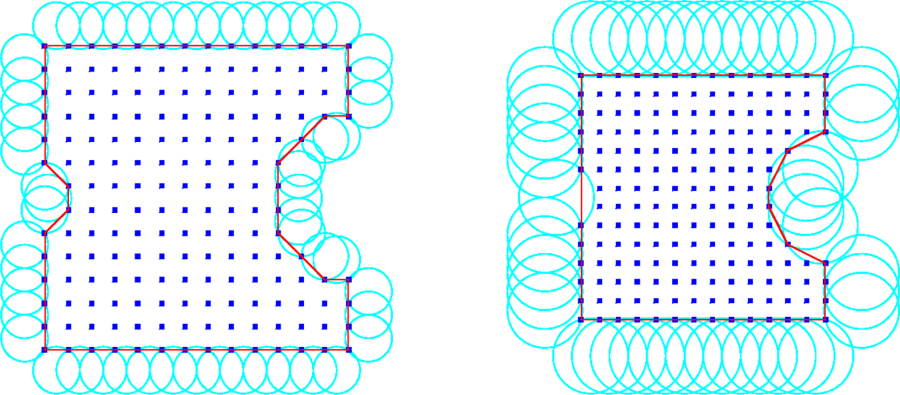
\includegraphics[width=0.7\textwidth]{figures/alpha_shape2D.png}
  \end{center}
  \caption{\textbf{Bisection in target PS \set{T}{}{}.} Algorithm \ref{alg:bisection} is run for the interval $[\variabile{q}^{\textrm{a}}, \variabile{q}^{\textrm{b}}]$ along direction $\variabile{p}=0$. The coordinates $\variabile{q}^{\textrm{c}}$ and $\variabile{q}^{\textrm{d}}$ are found such that 
$|\variabile{q}^{\textrm{c}}-\variabile{q}^{\textrm{d}}|<\textrm{tol}$. $\Pi^{\textrm{c}}= \Pi^{\textrm{a}}$ and $\Pi^{\textrm{d}}\neq \Pi^{\textrm{a}}$.}
\label{fig:bisec}
 \end{figure}
 Ciao \ref{fig:bisec}


%\appendix
%\include{chapters/Appendix_MC}
%\include{chapters/Sobol}
%\chapter{Exact intensity for the two-faceted cup}\label{app:boundariescup}
For very simple optical systems, the \textit{exact} target intensity of light can be calculated. Here we explain how this is done for the two-faceted cup with a Lambertian source described in Chapter \ref{chap:raytracing}. We remind the reader that, for this system, the intensity in a given direction $\variabile{p}$ in PS is defined as:
\begin{equation}\label{eq:eta_appendix}
I_{\textrm{PS}}(\variabile{p}) = \sum_{\Pi}\int_{\variabile{q}^\textrm{\,min}(\Pi, \variabile{p})}^{\variabile{q}^\textrm{\,max}(\Pi,\variabile{p})}L(\variabile{q}, \variabile{p})\textrm{d}\variabile{q} = \sum_{\Pi}\big (\variabile{q}^\textrm{max}(\Pi,\variabile{p})-\variabile{q}^\textrm{\,min}(\Pi,\variabile{p})\big )\,,
\end{equation}
where the sum is over all the possible paths, $\variabile{q}^\textrm{\,min}(\Pi,\variabile{p})$ and $\variabile{q}^\textrm{\,max}(\Pi,\variabile{p})$ are of the intersection points between the line $\variabile{p}=\textrm{const}$ and $\partial$\insieme{R}$_\textrm{t}(\Pi)$, and the second equation holds as we assume $L=1$ in \insieme{R}$_\textrm{t}(\Pi)$.
Therefore, if we are able to provide an analytic expression for the boundaries $\partial$\insieme{R}$_\textrm{t}(\Pi)$ we can calculated the position coordinates $\variabile{q}^\textrm{\,min}(\Pi,\variabile{p})$ and $\variabile{q}^\textrm{\,max}(\Pi,\variabile{p})$ analytically and we can compute the exact intensity for every direction $\variabile{p}$ is obtained using (\ref{eq:eta_appendix}). The procedure used for such purpose is explained next.
\section{Analytic approach}
The idea is to rotate the cup to determine the maximum number of reflections between a ray and the optical lines before reaching the target. The rays are considered to be straight lines instead of broken lines. Hence it is sufficient to find only one intersection point between the ray and a line segment (also in the case where more than one reflection occurs). Finally transforming (rotating or reflecting) back these points we obtain the corresponding coordinates at the target.\\ \indent
The two-faceted cup is defined in the $(\variabile{x}, \variabile{z})$-plane as in Chapter \ref{chap:raytracing}. 
Let $\gamma\in(0, \pi/2)$ be the angle that the left and right reflector make with the normal to the source. 
%\begin{figure}[t]
%\label{fig:cup}
%  \begin{center}
%%\vspace{-1.5cm}
%  \includegraphics[width=6.7cm]{cup.pdf}
%  \end{center}
%%\vspace{-2cm}
%  \caption{\textbf{Shape of the two-faceted cup.}  Each line of the system is labeled with a number.
%   The source \point{S}$= [-2,2]$ (line number $1$) is located on the $\variabile{x}$-axis.
%   The target \point{T}$= [-17, 17]$ (line $4$) is parallel to the source and is located at a height $\variabile{z}= 40$.
%   The left and right reflectors (line $2$ and $3$) connect the source with the target.}
%  \label{fig:cup}
%\end{figure}
The maximum $\variabile{z}$-coordinate that the two-faceted cup can reach during the rotation is defined by the $\variabile{z}$-coordinate of the point $\point{P}=(0,Z)$:
\begin{equation}\label{rotation}\begin{tabular}{llll}
$Z$ & $=$ & $ \big(h+\frac{\variabile{a}}{\tan\gamma}\big)\frac{1}{\cos\gamma}-\frac{\variabile{a}}{\tan\gamma}$ \\ $ \quad$ & $ \quad $ & $ \quad $ \\$ \quad$ &  $=$ & $\frac{h}{\cos\gamma}+\frac{\variabile{a}(1-\cos\gamma)}{\sin\gamma},$\end{tabular}
\end{equation} and $\point{R}=(0,-\frac{\variabile{a}}{\tan\gamma})$ is the rotation point. We define $\point{B}_k$ as the clockwise ($k<0$) or counterclockwise ($k\geq 0$) rotation image of $\point{P}$ around the point $\point{R}$ over an angle $\alpha_k=(2k+1)\gamma$, with $k$ an integer number (Figure \ref{fig:twofaced} is illustrative).
\begin{figure}[t]%\label{fig:twofaced}
 \centering
  \includegraphics[width=\textwidth]{rotated_cup.pdf}
 \caption{\textbf{The two-faceted cup rotated twice on both sides.} The line segment with end points $B_{k-1}$ and $B_{k}$ is the $|k|$ times rotated target. The coordinates $(q,h)$ on the target $B_{-1}B_{0}$ are obtained by transforming the coordinates $(u,v)$ of the intersection point between a ray and the segment $B_0B_1$ . The point $\point{R} = \big(0,-\frac{a}{\tan{\gamma}}\big)$ is the center of the circle described by rotating the cup (dashed line).}
  \label{fig:twofaced}
  \end{figure}
  %as the notation used in equation ($\ref{Bk}$) could suggest.
The position coordinates of points $\point{B}_k = (B_{k,x}, B_{k,z})$ are given by:
\begin{equation}
 \begin{pmatrix} B_{k,x}  \\  B_{k,z}\end{pmatrix}= -
  \begin{pmatrix} 0  \\  \frac{a}{\tan\gamma}\end{pmatrix}+
 \left(\begin{split}  & \cos\alpha_k  & -\sin\alpha_k \\  & \sin\alpha_k & \cos\alpha_k\end{split}\right).
 \begin{pmatrix}  0 \\  Z+\frac{a}{\tan\gamma}\end{pmatrix},
\end{equation}
The maximum number of reflections $r_{\textrm{max}}$ a ray can undergo before arriving at the target is:
\begin{equation}
r_{\textrm{max}}=\max\{k\in\mathbb{N} \;| \; B_{k-1,z}\geq 0\}.
\end{equation}
For example, for the two-faceted cup depicted in Figure \ref{fig:cup}, we found $r_{\textrm{max}}=2$.\\ \indent 
Given the coordinates $(\variabile{x}_1, \variabile{z}_1)$ and the angular coordinate $\optangle_1$ of a ray at the source, we can calculate the corresponding position $(\variabile{x}, \variabile{z})$ and direction coordinate $\optangle$ at the target as explained in the following. \\ \indent We compute the coordinates $(u,v)$ of the intersection point between the ray parametrization and the $|\variabile{k}|$ times rotated or reflected target $\point{B}_{\variabile{k}-1}\point{B}_\variabile{k}$ for which the intersection with the forward ray is not empty, for $\variabile{k}=-\variabile{r}_{\textrm{max}}-1, \cdots, \variabile{r}_{\textrm{max}}$. Next, if $\variabile{k}$ is even, the corresponding coordinates $(\variabile{x},\variabile{z})$ at the target are found by rotating back the coordinates $(\variabile{u},\variabile{v})$, otherwise a reflection is applied. Therefore, the ray coordinates $(\variabile{x},\variabile{z})$ at the target are given by:
\begin{equation} \label{rotation_target}\begin{pmatrix} \variabile{x}\\ \variabile{z}
\end{pmatrix} = \left(\begin{array}{cc}(-1)^k & 0  \\ 0 & 1\end{array}\right)
\left(\begin{array}{cc}\cos(-2\variabile{k}\gamma) & -\sin(-2\variabile{k}\gamma) \\\sin(-2\variabile{k}\gamma) & \cos(-2\variabile{k}\gamma)\end{array}\right)\begin{pmatrix} \variabile{u} \\
 \variabile{v}+\frac{a}{\tan(\gamma)}\end{pmatrix}-\begin{pmatrix}0 \\ \frac{a}{\tan\gamma}\end{pmatrix}.
\end{equation} We observe that the sign in the first matrix depends on the parity of $\variabile{k}$. When $\variabile{k}=0$, i.e., the ray does not reflect, the first matrices become the identity matrix and the cup is not rotated nor reflected. When $\variabile{k}$ is even, the determinant of the matrix given by the product between the first and the second matrix (\ref{rotation_target}) is equal to $1$ and we obtained a rotation matrix, while when $\variabile{k}$ is odd the determinant of the product matrix is $-1$ and we have a reflection matrix.
\\ \indent
The method of transforming the cup instead of the rays allows us to determine the positive luminance regions $\mbox{\insieme{R}}_1(\Pi_{\variabile{j}})$ and $\mbox{\insieme{R}}(\Pi_{\variabile{j}})$ in source and target PS, where every path $(\Pi_{\variabile{j}})_{\variabile{j}=1, \cdots, 2\variabile{r}_{\textrm{max}}+1}$ corresponds to $|\variabile{k}|$ reflections. The corresponding boundaries only consist of rays that either leave the extremes of the source or hit one of the points $\point{B}_\variabile{k}$. 
%At the boundaries a small change in the position or direction ray coordinate can cause a difference in the number of the reflections. 


Rays that leave the interior of \point{S} and hit $\point{B}_\variabile{k}$ have as position coordinates in source PS $\variabile{q}_1 = \variabile{x}_1\in(-\variabile{a}, \variabile{a})$, the corresponding target PS coordinates are $\variabile{q} = \variabile{x} = B_{\variabile{k}, \variabile{x}}$.
The direction coordinates of these rays at the source PS are $\variabile{p}_1 = \sin(\optangle_1)$ where $\optangle_1$ is given by:
\begin{equation}\label{anglesource}
\optangle_1 = \arctan\bigg(\frac{\variabile{x}_1-B_{k,x}}{B_{k,z}}\bigg).
\end{equation}
The corresponding direction coordinates at the target PS are $\variabile{p}=\sin(\optangle)$ where $\optangle$ is given by:
\begin{equation}\label{teta}
\optangle=(-1)^\variabile{k}(\optangle_1-2\variabile{k}\gamma).
\end{equation}

Rays emitted from the end points of the source have a constant position coordinate $\variabile{q}_1 = \variabile{x}_1 = \textrm{const}$ in source PS and varying a direction coordinate $\variabile{p}_1 = \sin(\optangle_1)\in[-1, 1]$ where $\optangle_1\in[-\pi/2, \pi/2]$. The corresponding target position coordinate $\variabile{x}$ is obtained from (\ref{rotation_target}) while the direction coordinate in the target PS is $\variabile{p} = \sin(\optangle)$, where $\optangle$ is given by Equation (\ref{teta}).
Note that the rays emitted from the end points of the source form vertical lines in source PS as $\variabile{q}_1= \textrm{const}$ and $\variabile{p}_1\in[-1,1]$ varies.
On the other hand, rays that hit points $\point{B}_k$ form vertical lines in target PS as $\variabile{q} = \textrm{const}$.
\\ \indent 
%In Figure \ref{fig:raggi} are shown some rays that compose the boundaries of $M_{\textrm{s},k}$ which coordinates are:
%$$ \begin{array}{cc}ADE = \Bigg(-a, \arctan\Big(\frac{-a+b_{-1,x}}{b_{-1,z}}\Big)\Bigg),\; ACE = \big(-a, \sin(\gamma)\big),\; AF = \big(-a, -\sin(\delta)\big), \\
% BCF = \Bigg(a, \arctan\Big(\frac{a-b_{1,x}}{b_{1,z}}\Big)\Bigg), BDF = \big(a, - \sin(\gamma)\big) \, \;\mbox{and} \,\; BE = \big(a, \sin(\delta)\big).\end{array} $$
%\begin{figure}
%\includegraphics[scale=0.55]{raggi6.jpg}
%\caption{\footnotesize{Rays that leave the corner points of the source. The rays $AF$, $BE$, $ACE$, $BDF$ are rays that do not hit the reflectors of the system.
%They constitute rays on the boundaries of the regions $M_{\textrm{s},0}$, $M_{\textrm{s},1}$ and $M_{\textrm{s},-1}$.
% The rays $ADE$ and $BCF$ are rays that hit once the reflectors of the system. They constitute rays on the boundaries of the regions
% $M_{\textrm{s},-1}$, $M_{\textrm{s},-2}$, and $M_{\textrm{s},1}$ or $M_{\textrm{s},2}$, respectively.}}
%\label{fig:raggi}
%
%\end{figure}
%$$ \begin{array}{cc}ADE = \big(-b, -(t_1+2\gamma)\big)),\; ACE = \big(-b, \sin(\gamma)\big),\; AF = \big(-b, -\sin(\delta)\big), \\
% BCF = \big(b, -(t_2-2\gamma)\big), BDF = \big(b, - \sin(\gamma)\big) \, \;\mbox{and} \,\; BE = \big(b, \sin(\delta)\big).\end{array} $$
% where $t_1 = \arctan(\frac(-a+b_{-1,x}{b_{-1}}))$ and $t_2 = \arctan(\frac(a-b_{-1,x}{b_{-1}}))$.
The boundaries at the source and target PS are shown in red in Figures \ref{fig:boundary} and \ref{boundaries_target}, respectively. 
\begin{figure}[htbp]
\centering
%\begin{minipage}[t]{.40\textwidth}
\includegraphics[width = 0.8 \textwidth]{analytic_boundaries_source}
\caption{Regions in source PS formed by rays that reflect $|k|$ times, for the two-faceted cup in Figure \ref{fig:cup}.}
\label{fig:boundary}
%\end{minipage} \qquad \qquad
%\begin{minipage}[t]{.40\textwidth}
\end{figure}
\begin{figure}[htbp]
\centering
%\begin{minipage}[t]{.40\textwidth}
\includegraphics[width = 0.8 \textwidth]{analytic_boundaries_target}
\caption{Regions in target PS formed by rays that reflect $|k|$ times, for the two-faceted cup in Figure \ref{fig:cup}.}
\label{boundaries_target}
%\end{minipage} \qquad \qquad \qquad
\end{figure}
%\noindent 
%Figure \ref{fig:boundary} and \ref{boundaries_target} show also the symmetry of the regions $M_{\textrm{s},k}$ and $M_{\textrm{t},k}$. 
%Finally we note that, since $k = 1$ is odd, the position of the regions $M_{\textrm{t},1}$ and $ M_{\textrm{t},-1}$ are exchanged with respect to the position of $ M_{\textrm{s},1}$ and $ M_{\textrm{s},-1}$.
Once the boundaries at the target are determined, the coordinates of the intersection points between line $\variabile{p}=\textrm{const}$ and $\partial$\insieme{R}$(\Pi_{\variabile{j}})$ are found for every path $(\Pi_\variabile{j})_{\variabile{j}=1, \cdots, 2\variabile{r}_{\textrm{max}}+1}$ along every direction $\variabile{p}$. The target intensity is computed using Equation (\ref{eq:eta_appendix}). The intensity profile is depicted in Figure \ref{fig:intensity_cup_analytic}. 
\begin{figure}[t]
\centering
%\begin{minipage}[t]{.40\textwidth}
\includegraphics[width = 0.7\textwidth]{Exact_intensity}
\caption{Profile of the exact intensity at the target of the two-faceted cup.}
\label{fig:intensity_cup_analytic}
%\end{minipage} \qquad \qquad \qquad
\end{figure}
Since the boundaries are computed analytically, the intensity $I(\variabile{p})$ found is the exact intensity.

The exact intensity found as described above was taken as reference intensity in Chapters \ref{chap:triangulation} and \ref{chap:raymapping1}.




\chapter{Introduction}
\label{chap:Introduction}
%\section{Motivation}   
%\label{sec:Motivation}
The mesolimbic dopamine pathway comprising the ventral tegmental area (VTA) and projection terminals to the ventral striatum (VS) has been identified as a critical neural system involved in processing both the rewarding and aversive behavioral effects of rewarded and unrewarded stimuli (\cite{Schultz1992}, \cite{Montague}, \cite{Ungless2004}, \cite{Sun2014}, \cite{Tobler2003}, \cite{UchidaDop1}, \cite{Takahashi2016}). In these functions the brain performs simple arithmetic: it compares the expected and the received outcomes and computes the differences between the two. In other words after receiving the outcome, it computes the error made in predicting the outcome. This signal is called reward prediction  error (RPE): being essential to learning, to reward maximization, and to guide reward-related behavior, RPE has been widely investigated in last decades (\cite{Schultz1997},, \cite{UchidaDop}, \cite{Fiorillo}, \cite{Pagnoni}, \cite{Schultz2016}). In dopamine neurons RPE signals are characterized by activations following primary food and liquid rewards, and visual, auditory and somatosensory reward-predicting stimuli. Dopamine neurons fire phasically (100-500 ms) after unpredicted rewards or cues that predict reward. Their response to reward is reduced when a reward is fully predicted (\cite{Uchida}). The uncertainty about the reward outcome is critical in the measure of information and in assessing the accuracy of predictions. The uncertainty is determined by the probability P to get the reward, and its maximal at $P=0.5$, while decreases at higher and lower probabilities.\\Fiorillo and collaborators used distinct stimuli indicating the probability of reward, to show that the phasic activation of dopamine neurons varied monotonically across the full range of probabilities (\cite{Fiorillo}). Figure \ref{fig:probDopamine} (left) displays the dopamine neurons response to stimuli with different reward probability. These observations have defined the basis of the current knowledge on dopamine neurons, which are assumed to signal discrepancies between expected and actual rewards, in other words they are thought to compute the reward prediction error (RPE).\\Being essential to learning, since ever RPE signals picked the scientist$'$ curiosity, who dissected the evolution in time of those signals to understand the underlying nature of multiple time components of RPE. The reward-related activation is usually preceded by a brief detection component before the proper valuation of stimulus: the RPE signal evolves in time from unselective sensory detection to more demanding and crucial stages of identification and valuation (\cite{Tobler2003}, \cite{Nomoto2010}, \cite{Fiorillo2013}, \cite{Schultz2016}), value that is constantly adapted during the learning process by dopamine neurons (\cite{Tobler2005}). The initial component, characterized by a brief activation, occurs unselectively in response to a large variety of unpredicted events and corresponds to the large range and heterogeneous nature of potentially rewarding stimuli and object present in the environment.
\begin{figure}[H]
    \centering
    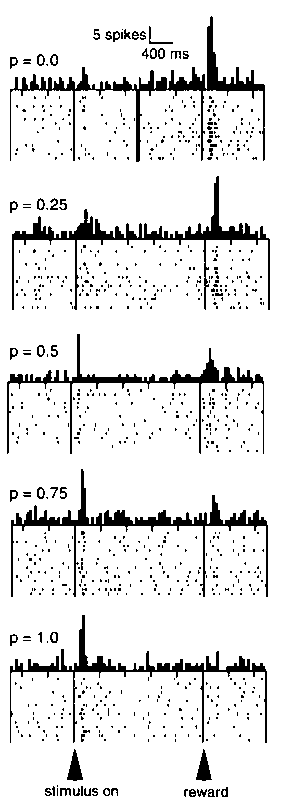
\includegraphics[scale=0.6]{figures/Schultz1.png}
    \hspace{1.5cm}
    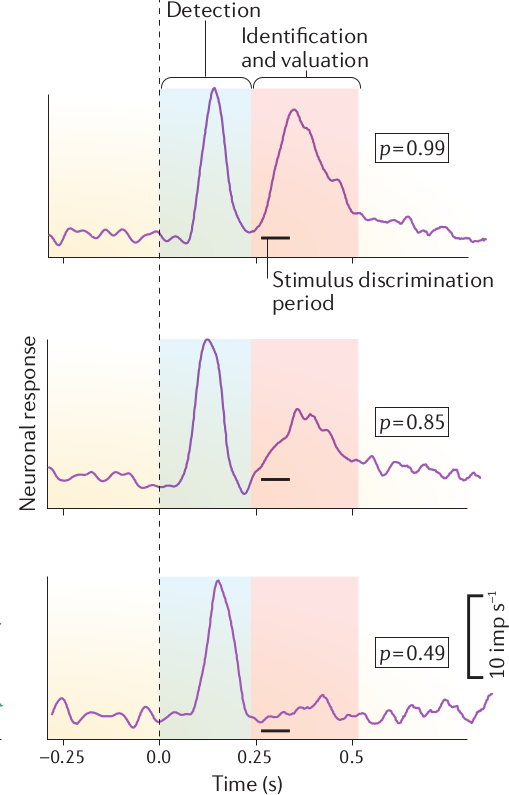
\includegraphics[scale=0.35]{figures/ResponseProbSchultz.png}
    \caption{\textbf{Left:} Adapted from \cite{Fiorillo}: Reward-related responses of dopamine neurons. Distinct stimuli were used to indicate the probability of reward (p increasing from top to bottom). Dopamine neurons signals varied monotonically across the full range of probabilities. At the stimulus onset, the dopamine response increased monotonically as the probability increased; at the reward time instead, the dopamine response decreased monotonically as the probability increased. \textbf{Right:} Adapted from \cite{Schultz2016}: A demanding random dot motion discrimination task reveals completely separated dopamine response components. Larger responses correspond to higher reward probabilities (p). The initial, stereotyped, non-differential activation reflects stimulus detection and decreases back to baseline (blue zone); the subsequent separate, graded increase develops when the animal signals stimulus discrimination; it codes reward value (red zone), which in this case derives from reward probability}
    \label{fig:probDopamine}
\end{figure}
This component reflects the detection of stimulus, regardless its relation with the reward.\\The second component, also called main component or valuation component, defines the function of the dopamine response and reflects the evolving neuronal processing that is required to fully appreciate the value of the stimulus. Thus, at this stage the stimulus is identified and valued. Figure \ref{fig:probDopamine} (right) shows the separation between the detection salience and the valuation component of RPE signals in dopamine neurons.\\Like VTA neurons, VS neurons show as well reward-related response. In monkey experiments first it has been shown that VS neurons predominantly fire in relation to the expectation of reward, regardless of the movement/no-movement reaction (\cite{Schultz1992}). This signals suggested that VS neurons evaluate reward and reward-associated stimuli, and thereby participate in the processing of information underlying the RPE computation.\\The stereotypical responses of striatal projection neurons in VS during learning consist of a sustained increase of activity before the occurrence of the reward delivery (see figure \ref{fig:StriatumN}).
\begin{figure}[H]
    \centering
    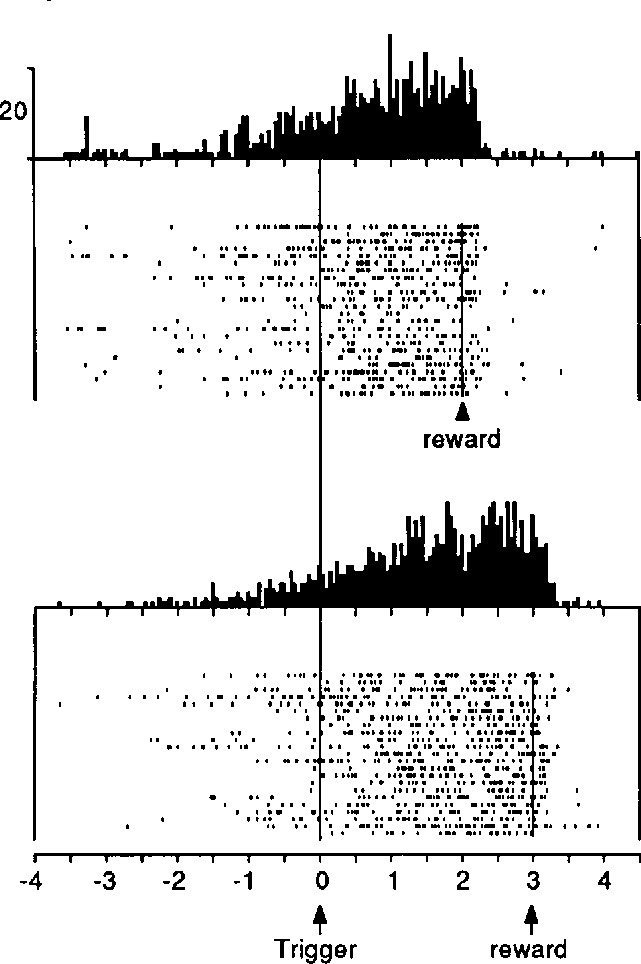
\includegraphics[scale=0.22]{figures/StriatumR.png}
    \caption{Adapted from \cite{Schultz1992}. Stereotypical reward-related VS neuronal activity. Effect of delayed reward delivery in no/ no go task in monkeys. VS neurons show sustained increases of activity before the occurrence of individual task events. VS neurons exhibit activation in relation to the expectation of reward.}
    \label{fig:StriatumN}
\end{figure}
The ventral pallidum (VP), from which neurons with fast spiking activity were recorded, is innervated by dopamine inputs from the midbrain and dopamine directly alters VP neuronal firing (\cite{Napier89}). Since 1991 VP was assumed to integrate reward-related signals carried by VTA dopamine neurons, involved in reward-motivated behavior (\cite{Napier91}). This concept was quickly expanded to encompass the idea that dopamine transmission within the VP regulates a collection of behaviors, including locomotion and cognition (\cite{Napier92}). Contrary to the well-characterized, relatively homogeneous projection neurons dominating striatum, the cellular architecture of VP is only beginning to be understood in terms of their heterogeneous cell-types, neurotransmitters, and connectivity (\cite{Heimer1997}, \cite{Tachibana2012}). In other studies conducted in our lab, it was observed that VP units displayed either purely excitatory, purely inhibitory, or multiphasic excitatory and inhibitory responses to the same stimulus or across reward and unrewarded stimuli (unpublished results). For these reasons, the responses of VP neurons are expected to be diverse among different VP units.\\While there exist an extensive literature on how RPE signals are expressed by single units, how the RPE computations are implemented in VS-VTA neural circuits remains elusive. Thus, better understanding VS-VTA related circuits, will broaden our understanding on the underpinnings of RPE signals.\\In this work I studied the formation of prediction error signals in interregional assemblies during reinforcement. Towards this aim, I used dual site electrophysiological in-vivo data from VS (including ventral pallidum) and VTA, during a reversal go/no go task in mice.\\On this data set I applied a cell assembly detection algorithm (\cite{RussoDurstewitz}). The novel statistical approach was built to detect spike patterns at any time scale and coordination, enabling so the investigation of the time scales and the inter-units lag activation involved in the detected patterns of spikes. I focused the analysis on interregional assembly-pairs, namely assembly formed by two neurons, one in VS and the other in VTA. In this way I were able to examine the directionality between VS-VTA interactions through the inter-unit lag activation.\\I found that, in interregional assembly-pairs, VS predominantly led VTA. Moreover interregional assembly-pairs showed a bimodal time scale distribution, such bimodality was solely present in VS-VTA pairs and did not emerge in intraregional pairs.\\I examined the assembly-pair activity patterns of pairs with different time scales and directionalities. It emerged that different time scales and directionalities segregated different activity patterns. Specifically, in more precise time scale, directional assembly-pairs with VTA following VS showed excitatory responses following reward-predicting stimuli, in agreement with prediction error encoding.\\Taking advantage of neuron types classifications both in VS and VTA, I further investigated the specific cell-type composition of the assemblies exhibiting directionality. Interestingly only assembly-pairs formed by putative striatal projection neurons (pSPN) and dopamine neurons (pDAN) were directional in the direction of VS leading VTA.\\Thus, I looked at the task related activity patterns of different assembly-pair types; and I expected that, being directional, SPN-DAN assembly-pairs could exhibit RPE response.\\Indeed, different assembly-pairs types showed different activity patterns in response to external potentially rewarded stimuli. The segregation reflected different encoding features in different assembly-pair types.\\In particular, SPN-DAN assembly-pairs were mainly activated by the rewarded stimulus, and only a small fraction ($\sim12\%$) was activated by both stimuli. The activation started few hundred milliseconds after the stimulus onset and remained high for few hundred milliseconds ([100,400] ms). SPN-DAN activity pattern suggested that those pairs conveyed the valuation component of RPE signals (\cite{Tobler2003}, \cite{Nomoto2010}, \cite{Schultz2016}). Conversely, FSN-DAN assembly-pairs responded indistinctly to both stimuli, either showing a brief and phasic activation at the stimulus onset or being inhibited by one or both stimuli; these signals suggested that FSN-DAN pairs were involved in motivational and/or hedonic signals. Hence, I put forth the hypothesis that the assembly-pairs specialize in different aspects of the learning-related coding.\\%\\Detailed discussion will be presented in\hyperref[sec:TaskResp]{~Section \ref*{sec:TaskResp}} and\hyperref[sec:FalseAlCorrRej]{~Section \ref*{sec:FalseAlCorrRej}}.\\
So far the description barely considered the dynamic of the learning process. In fact, reward prediction coding signals in dopamine neurons varied according to the probability to get the reward, which was often related to the uncertainty (\cite{Schultz1992}). Dopamine neurons in VTA as well as neurons in VS modified their activity in function to the difference between received and expected outcomes (\cite{Fiorillo}). In similar ways, far from being static, the assembly-pair activity modified itself trial by trial, reflecting the dynamic of the learning.\\This dynamic could not be replicated by the study of activity patterns, for this reason I modeled a reinforcement learning model. Crucial terms of reinforcement learning are the uncertainty of the animal to get the reward and the reward prediction error; the first is high when the animal is unsure about the outcome, and decreases as the animal becomes expert; the latter term reflects the ability of the animal to predict the reward: as the animal learnt is supposed to be able to predict the future outcomes. Both the aforementioned terms were modeled as time evolving components, in such a way that I could take into account the fact that, during the task, the animal had to assign and re-assign new value to the presented stimulus.\\Based on broad knowledge, reward prediction error signals are thought to be anti-correlated with the uncertainty of the animal to get the reward and correlated with the prediction error term of the Rescorla-Wagner models.\\Thus, if SPN-DAN assembly-pairs specifically encoded prediction error signals, I expected their activity to anti-correlate with the modeled uncertainty ($\alpha$) and to correlate with the modeled prediction error ($\delta$).\\Imodeled two linear Poisson regressions and I regressed the assembly-pairs activity on $\alpha$ and $\delta$. Our SPN-DAN assembly-pairs indeed anti-correlated with the uncertainty and correlated with the prediction error term. Furthermore I noted that such correlations were not found in other assembly-pair types, from which I could conclude that SPN-DAN assembly-pairs specifically conveyed reward prediction signals.  

%\include{chapters/LiyaData}
\chapter{Odor discrimination task in mice}
\label{chap:MaxData}
%\section{Introduction}
Neuronal models of reinforcement learning assume interactions of midbrain dopaminergic neurons and striatum to compute the differences between anticipated and expected outcomes. The nature of this cross-areal interaction is however not fully understood. On this purpose we present an application of the cell-assembly algorithm, at level of pairs, on electrophysiological data from mice.
Dual side in-vivo recordings of electophysiological activity from Ventral Striatum, including Pallidum, (VS) and Ventral Tegmental Area (VTA), allowed us to study directionality between the two regions.
The novel statistical approach presented treats the temporal scale and precision of coherent activity patterns as free parameters, to be determined from the data, thus, instead to make assumption, we deduced from data temporal scales and precision involved in assemblies pairs with units either from both regions or from only one of the two regions, shedding light on VS-VTA interaction temporal structure and directionality.
Taking advantage of well defined neuron typologies classifications both in VS and VTA, we further investigated the specific cell-type composition of the assemblies exhibiting directionality. 
%According to their response properties, neurons in VTA are classified in Type I (dopaminergic), Type II(GABAergic) and Type III; according to their electrophysiological properties, neurons in VS are di-vided in medium spiny neurons (MSN), cholinergic interneurons (CIN), and fast spiking interneurons(FSI), the latter are mostly pallidal units.
\section{Description of experiment and data set}
The task presented is a go-no go reversal odor discrimination task. Two odors were presented to the mouse, one rewarded (CS+) with reward probability 0.9, the other one not rewarded (CS-). Learning the task consisted in licking at least twice when CS+ was presented (hit trials) and not licking during or after the CS- presentation (correct rejection trials). Once the performance criterion was reached, contingencies were switched. Lick window was open for an interval ranging from 1500 $ms$ to 2000 $ms$ for different sessions after a delay from 500 $ms$ to 1500 $ms$. Only licks happening in the lick window interval were counted as valid to get the reward.
\begin{figure}
    \centering
    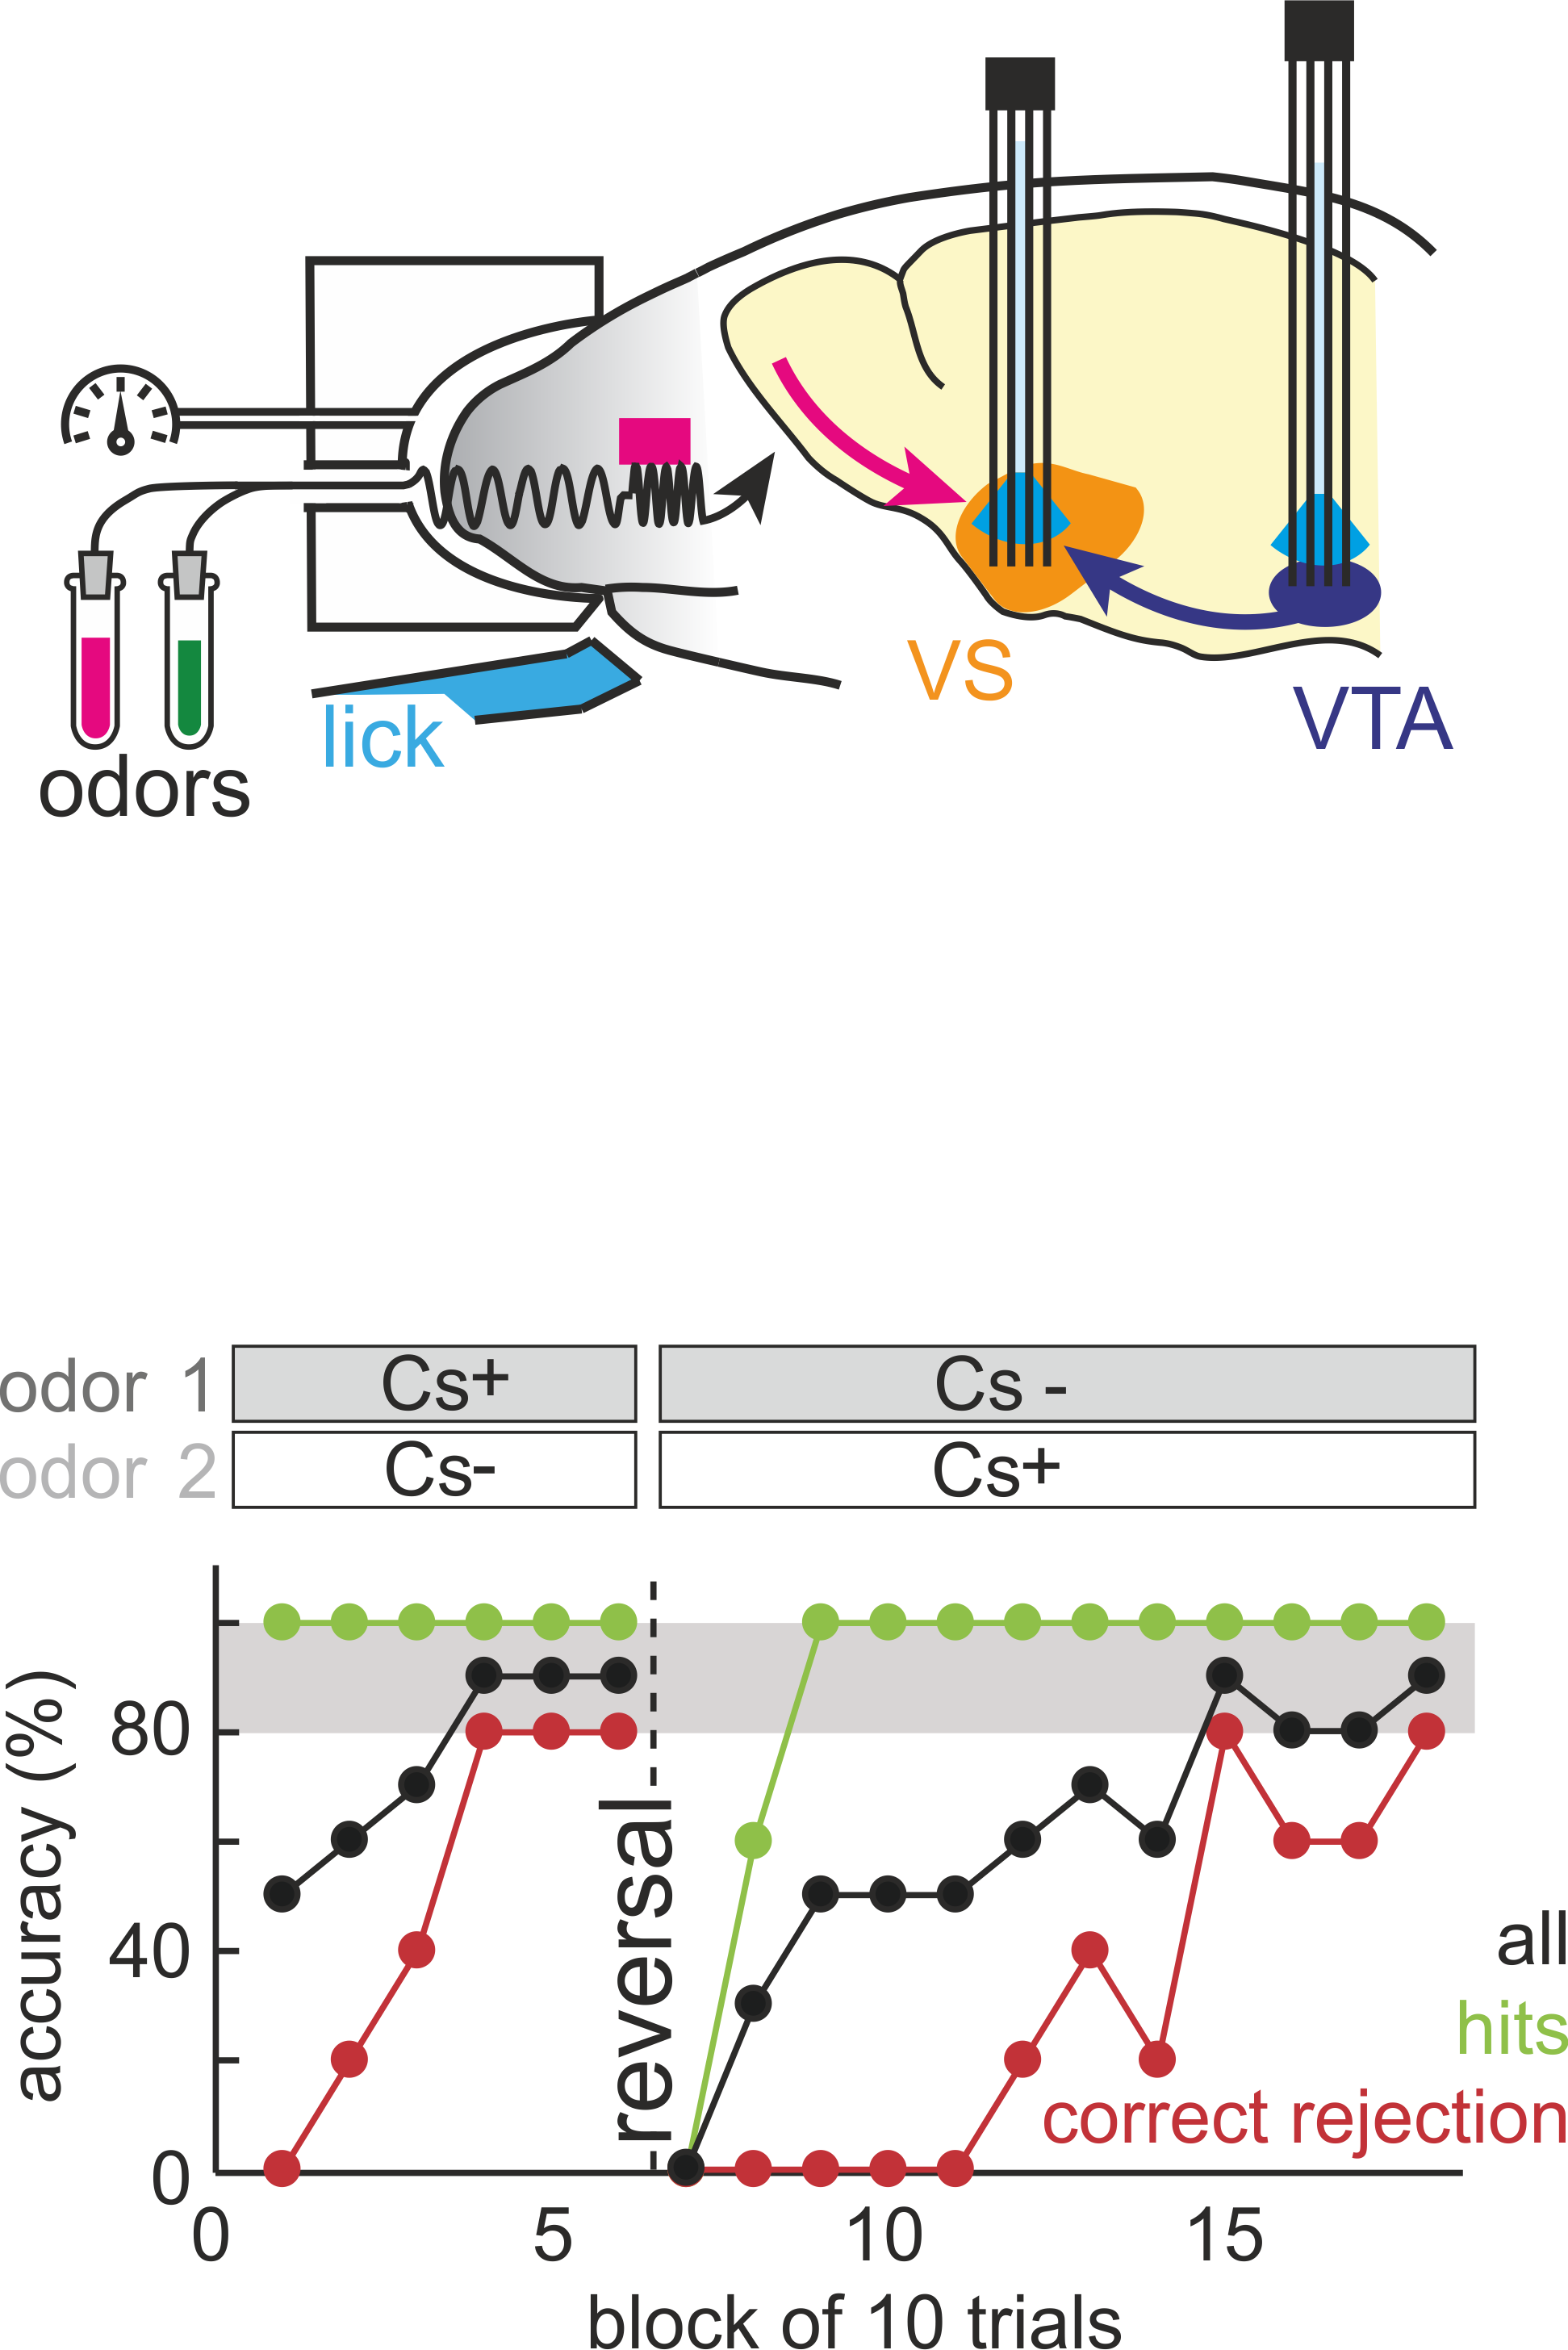
\includegraphics[scale=0.3]{figures/experiment.png}
    \caption{Experimental setup and mice performance}
    \label{fig:experiment}
\end{figure}
\section{Single cells analysis}
We have $803$ VS units and $272$ VTA units in total, that were classified in sub-typologies, specifically VS units were classified as either medium spiny neurons (MSNs), fast-spiking inter-neurons (FSIs) or cholinergic interneurons(CINs), according to their firing pattern characteristics computed using only spikes during the inter-trials interval and after session. Units with a firing rate higher than $12 Hz$ were assigned as FSIs and all units with a firing rate below $2 Hz$ as MSNs. Units in the remaining range were designed as putative regular-firing CINs if the CV or their $ISI$ distribution was less than $1.2$ and ISIs less than $60 ms$ contributed no more than $20\%$ of all ISIs. Finally the resting units were characterized as MSNs or FSIs if they ever were silent for more than $2 s$. Unsing this classification mean normalized autocorrelations and mean waveforms have canonical patterns ({\color{red}I don't know if I can borrow the figure from Max and whether put the figure here or in the appendix}). %(\ref{fig:AutoVS}).
VTA units were instead classified as Type I (Dopaminergic units), Type II (Gabaergic units), and Type III according to their task related activity using a clustering approach adapted from (\cite{Uchida}). First, response were characterized for the relevant time spans ({\color{red}ask Max for the updated intervals}(CS+ from 0 to 0.5 and US from -0.5 to 0 and from 0 to 0.5), significant task related response were assessed with Friedman test, and only significant units ($p<0.05$) were included in the clustering classification.{\color{red}part of classification has to be included}
%\begin{figure}
 %   \centering
  %  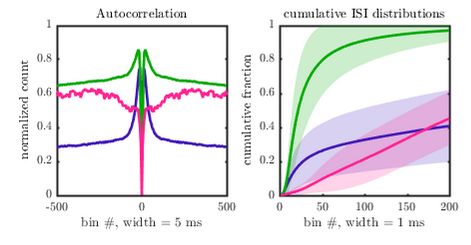
\includegraphics[scale=0.7]{figures/AutocorrelationVSunits.png}
   % \caption{Caption}
    %\label{fig:AutoVS}
%\end{figure}({\color{red}citation of graybiel 2005 if it is the rigth paper})
%distributed as shown in fig.(\ref{fig:GlobalPie})
\section{Preliminary cell assemblies results}
\begin{figure}
    \centering
    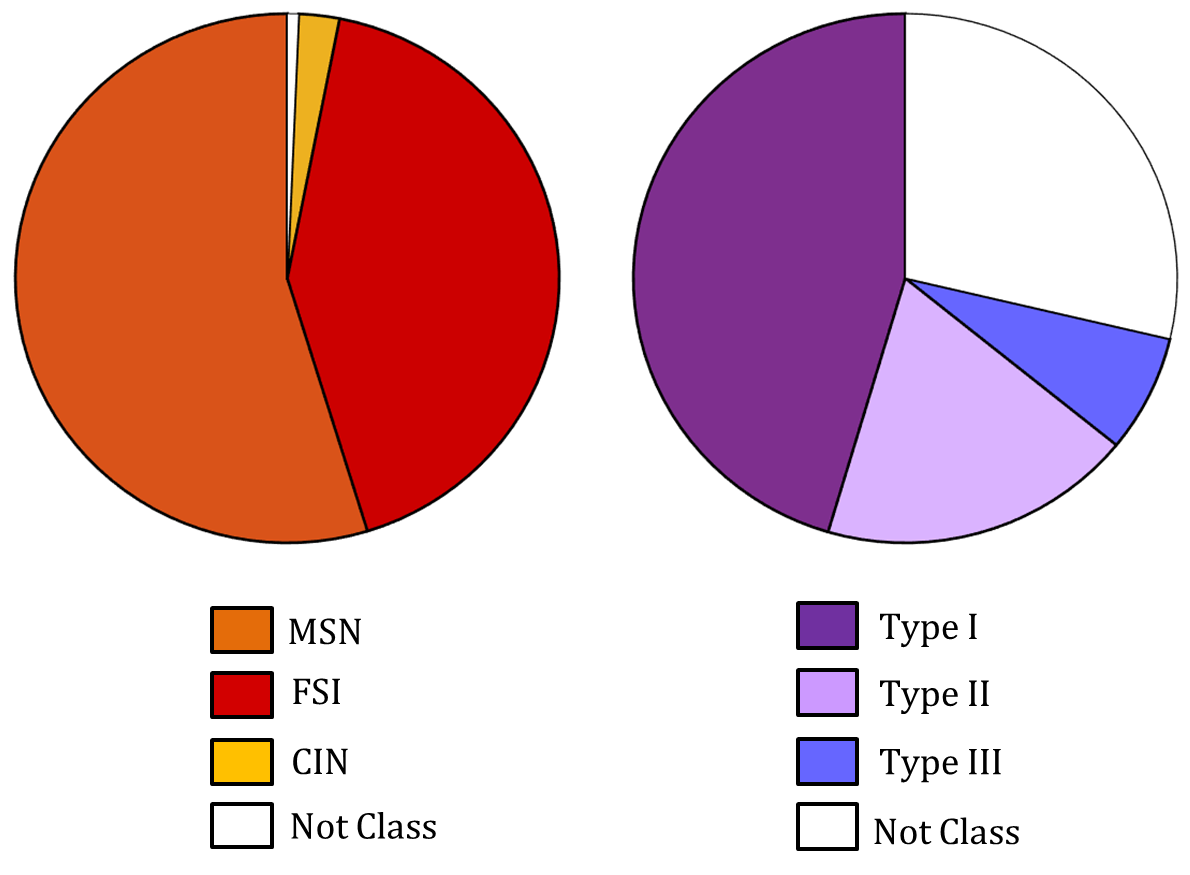
\includegraphics[scale=0.3]{figures/GlobalRegionPieandLegenda1.png}
    \caption{Pie charts of neuron typologies in VS and VTA }
    \label{fig:GlobalPie}
\end{figure}
Preliminary cell assemblies analysis were aimed to understand the size of the concentration of the shared pairs, namely how many units are involved in pairs and, among those, how the units typologies were distributed in assembly pairs. Classified units were distributed in the two regions as shown in fig. (\ref{fig:GlobalPie})

{\color{red} Include figure pie charts for all reversal paradigma}
\section{Time scales, directionality}
Applying the cell-assembly algorithm we were able to detect synchronous ($lag=0$) and asynchronous ($lag\neq 0$) cell assemblies at arbitrary time scale ($\Delta$). Time scales distribution results to be different for intra- regional assembly pairs (pairs with units from VS or VTA) and inter-regional assemblies pairs (pairs with units from both VS and VTA). It's important to point out that, in case of inter-regional pairs, the lag distribution it's a instruments to measure directionality between two regions, indicating which unit fires first leading the activation pattern activity and which one consequently follows. In our case $lag >0$ means VS precedes in activity VTA, and $lag <0$ the opposite, $lag=0$ means that the two units are  simultaneous in activation at the precision of the time scale at which are detected.
We start our analysis from time scales distribution involved in detection pairs.
\begin{figure}[H]
\centering
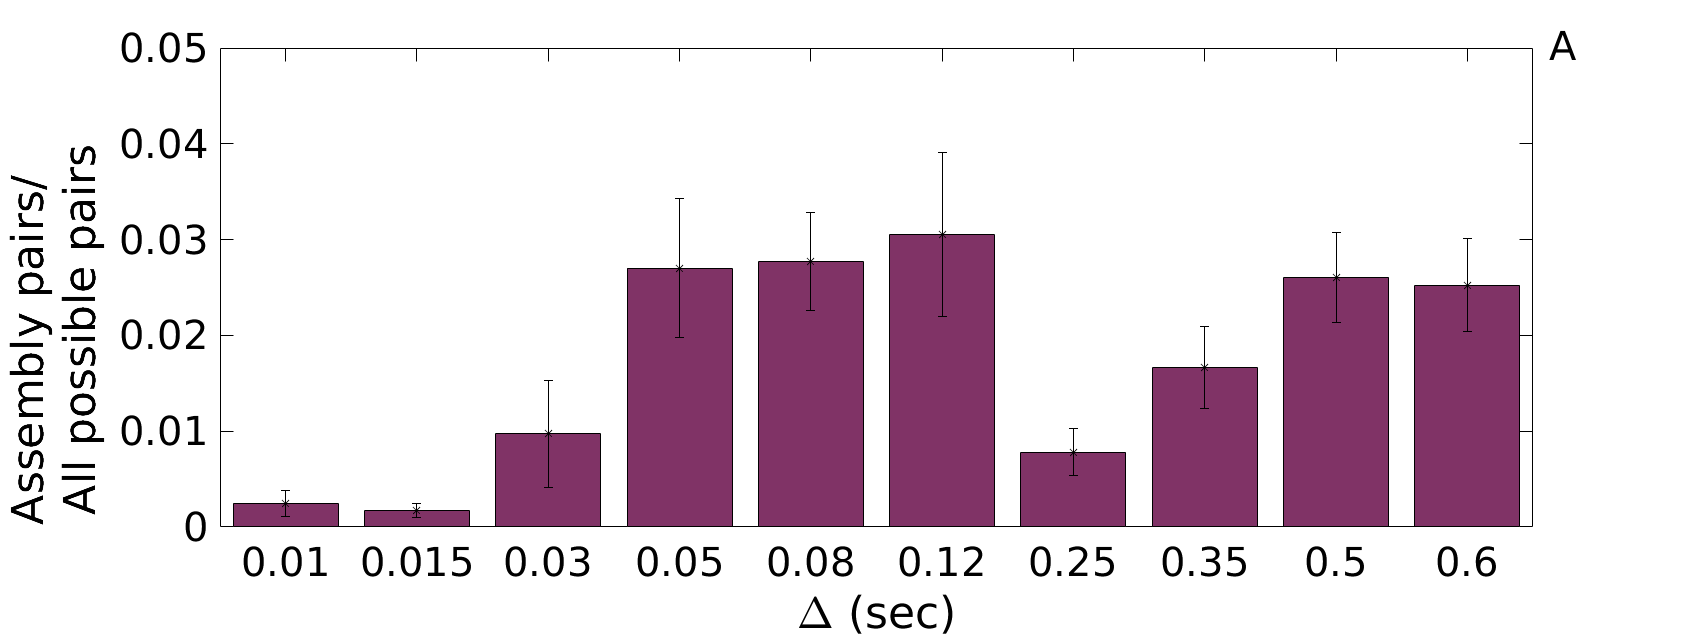
\includegraphics[scale=0.2]{figures/VS_VTA_SLet.png}
%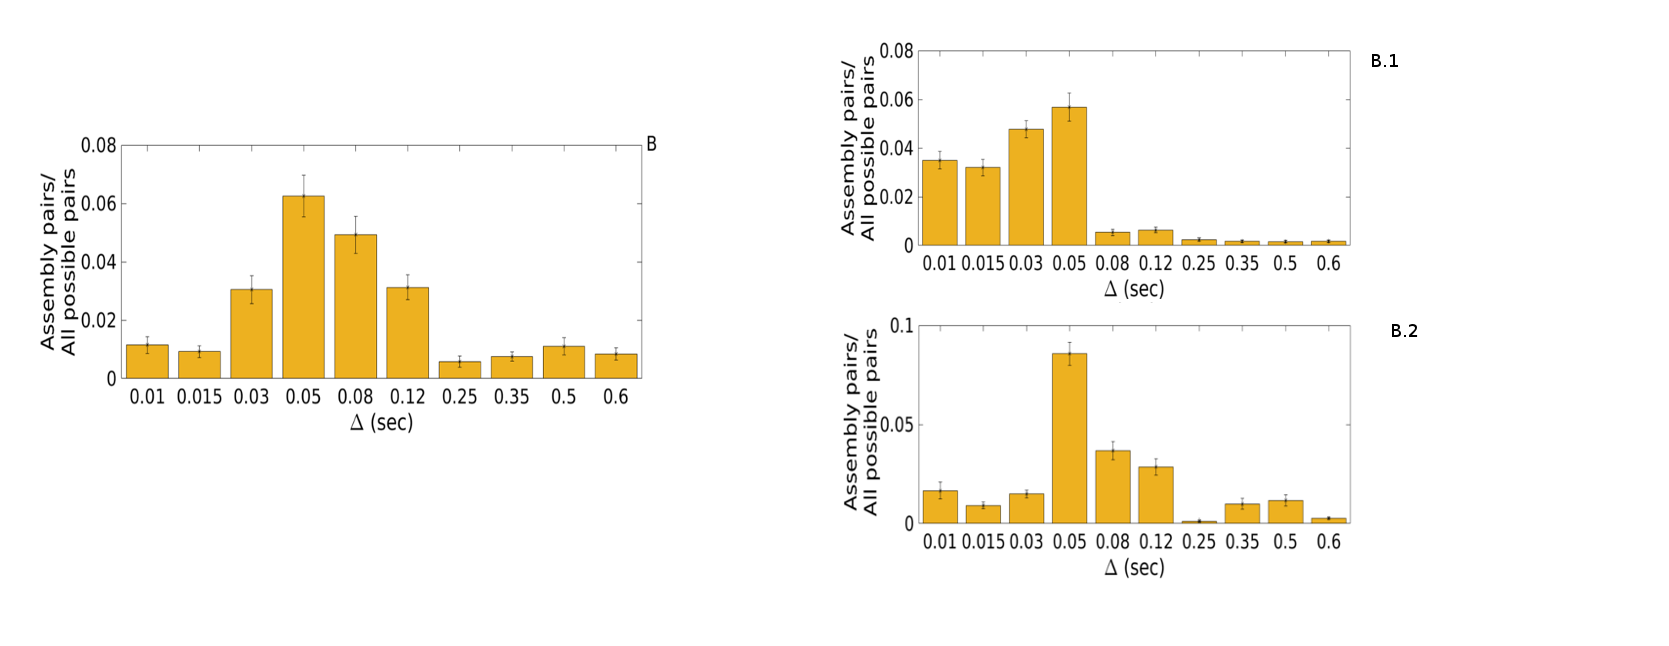
\includegraphics[scale=0.4]{figures/VS_VS_SLet1.png}
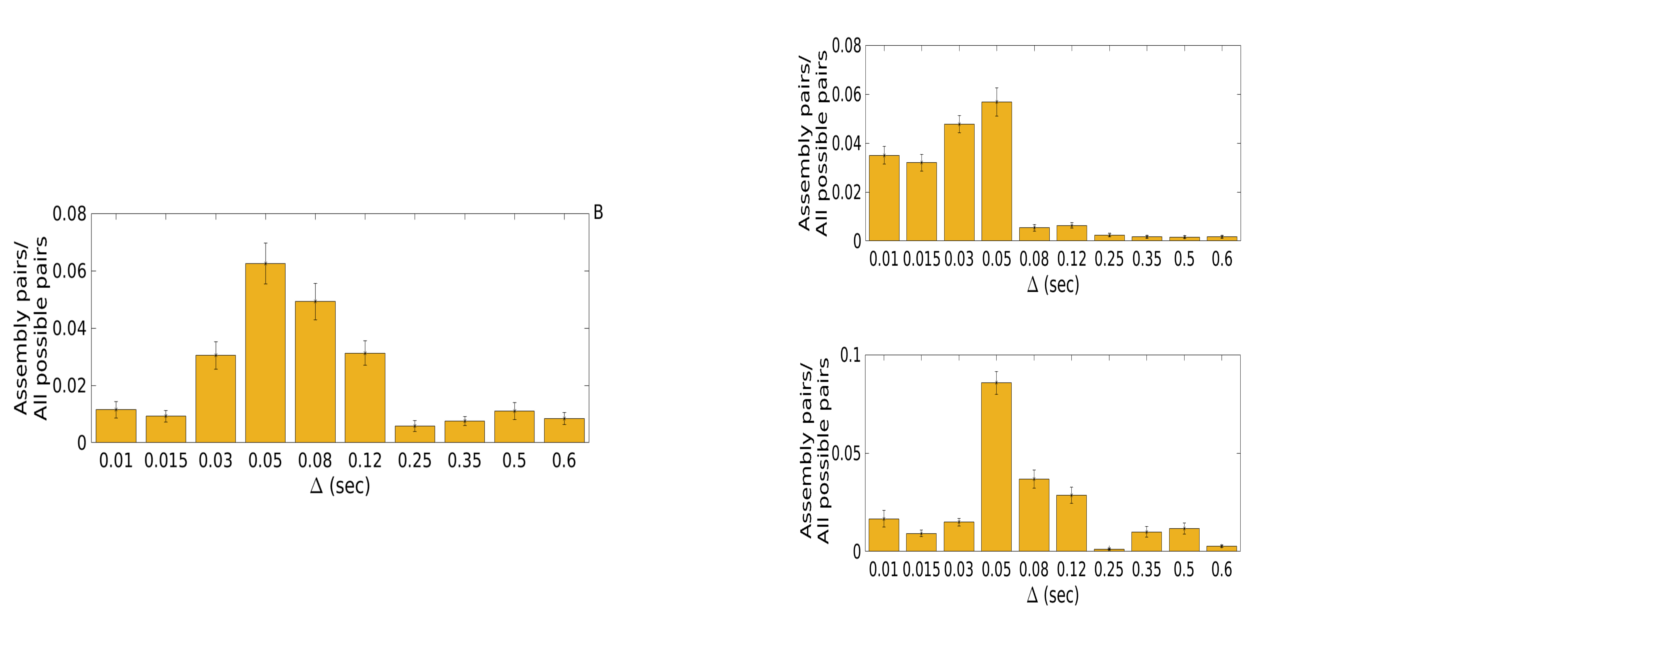
\includegraphics[scale=0.4]{figures/AllBinVSVS.png}
%\includegraphics[scale=0.2]{figures/VS_VS_SLet.png}
\includegraphics[scale=0.2]{figures/VTA_VTA_SLet.png}

\caption{{\color{red}Important!! Re do the figures with GIMPS include text with title} Bin distribution for intra-regional and inter-regional pairs. A) VS-VTA pairs show a bimodal distribution, meaning two temporal scale involved in inter-regional activtion patterns. B) VS-VS pairs bin distribution presents a peak at 50 $ms$, specifically in this region the pairs MSN-FSI high show an highly peaked distribution, almost centered at the peak of 50 $ms$, plot (B.2), while in MSN-FSI low distribution, albeit the peak is still at 50 $ms$, is evident the predominance of very precise time scales, including bins from 10 $ms$ to 50 $ms$, with respect to the larger time scale plot (B.1).}
\label{fig:BinDistr}
\end{figure}
Clear differences in time scales distribution of pairs detected in VS, VTA and VS-VTA emerge in fig.(\ref{fig:BinDistr}). While we observed assemblies of temporal precision at the scale of few tens of milliseconds only within either VS or VTA, assemblies of lower temporal precision were detected across VS-VTA units. The temporal precision of this last group displayed a bimodal distribution with peaks around $80$ milliseconds and one $1.6$ second, revealing the presence of two time scales, the first, preciser, ranged from 10 $ms$ to 250 $ms$, and the second including broader bin sizes. Intra-regional VTA-VTA pairs instead don't present any peak in time scales distribution. Intra-regional VS-VS bin size distribution is peaked around 50 $ms$. In VS we noticed differences between MSN and high-firing-rate FSI pairs and MSN and low-firing-rate FSI bin size distributions: specifically the firsts show higher temporal precision than the latter. {\color{red}{Include Figure of MSN-FSI and caption of bin size distribution}}.
Bin width and lags analysis reveals time scale segregation, that can reveal in turn different assembly-activation patterns. In fig.(\ref{fig:AsActBinLag}) heat maps of assembly activity show differences in activation patterns among different bin width and lag. In the paradigm in examination animals were well-trained, it was the third time that the same couple of odor were presented with the same stimulus duration length.
\begin{figure}
    \centering
    \includegraphics[scale=0.45]{figures/AsActPerBinLag1.png}
    \caption{Assembly-activation patterns given time bins and lags. In a.) totality of assemblies of one experimental paradigm, b,c,d. assemblies of same paradigm of a. selected for bin size ($\Delta$) and lag, $\Delta < 0.25 s$ and $lag > 0$ (b.), $\Delta > 0.25 s$ and $lag > 0$ (c.), $lag < 0$ (d.)}
    \label{fig:AsActBinLag}
\end{figure}
Directionality between VS and VTA was a point of particular interest for our study. The above consideration led us to study separately lag distribution of VS-VTA pairs detected in preciser and broader temporal scales highlighted from bin sizes distribution. 
Interestingly only the lags of more temporally precise assemblies displayed an asymmetric distribution indicating VS leading VTA (fig. \ref{fig:LagInSecAll}). Specifically, these directional assemblies were composed of striatal and pallidal projection neurons leading dopaminergic VTA neurons (MSN and Type I pairs). Importantly, inter unit activation lags of assemblies containing pallidal neurons (FSI) were shorter than those containing striatal projection neurons (MSN), compatibly with assumed connectivity.
\begin{figure}[H]
\centering
\includegraphics[scale=0.3]{figures/LagGeneralInSec.png}
\caption{Lag distribution for VS-VTA pairs in seconds. In green the synchronous pairs. On the left, lag distribution for pairs detected in preciser time scales. Slight distribution asymmetry indicates directionality in the direction of $lag > 0$, meaning a predominance of pairs in which VS leads VTA. On the right, the lag distribution for pairs detected in the broader time scale.}
\label{fig:LagInSecAll}
\end{figure}

\begin{figure}[H]
\centering
\includegraphics[scale=0.4]{figures/Type_oriz.png}
\includegraphics[scale=0.4]{figures/OnlyLaserOriz.png}
\caption{blabla}
\label{fig:LagInSecAll}
\end{figure}
In fig. (\ref{fig:directional_assembly}) a directional assembly. On top is shown mean and standard deviation of the assembly's activity for paired (grey line) and unpaired odor trials (purple line) in the original phase. On bottom raster plot and firing rate (mean and standard deviation) of units in assembly. x-axis origin correspond to the odor onset, while the red line marks the end of the stimulus duration. The examined assembly has a positive lag, that means VS preceding in activity VTA, from neuronal activity we can see in fact the VS unit activate before than the VTA unit. The assembly was detected with a bin size of $0.25 sec$, meaning that we are in the small temporal scale domain, in which the directionality clearly emerged. From the raster plot is evident that this kind of activation was persistent in each trial, in fact that assembly showed a significant task related activity after the stimulus. It is interesting to note the different activation for paired odor trials and unpaired odor trials, revealing the odor discrimination capability of the assembly. 
\begin{figure}
    \centering
    \includegraphics[scale=0.4]{figures/1_21Lastrev1Pru_An4Poster2.png}
    \caption{Directional assembly. On top mean and standard deviation of the assembly's activity for paired (grey) and unpaired odor trials (purple) in the original phase. On bottom raster plot and firing rate (mean and standard deviation) of units in assembly. x-axis origin correspond to the odor onset, while the red line marks the end of the stimulus duration. The examined assembly has a positive lag, that means VS preceding in activity VTA, from neuronal activity we can see in fact the VS unit activate before than the VTA unit.}
    \label{fig:directional_assembly}
\end{figure}
 To better study assemblies activation patterns we first selected the task relevant moments of the experiment, choosing as interval of interest period around the stimulus presentation and the reward delivery, then we analysed the task related assemblies activity in two experimental phases (original and reversal) noting diverse responses among neural typologies involved. 


%\section{Discussion}
%\section{Combination of single neuron and assemblies analysis}
%\subsection{Directionality using classification}
\subsection{Significant task related response for typology}
Our interest was focused again to the smallest temporal scale.
Here, the assemblies were pruned according their significant task related activity, that was tested with Friedman's test and a non parametric version of the repeated measures Anova. We preferred to use non-parametric tests to be free from the assumption of gaussianity of the observations. Results of the two tests were consistent each other. The two relevant events of the task were the odor onset and the reward delivery, then we choose whether the assemblies showed a significant activity in three windows: Post-Stimulus [0s, 0.5s], Pre-Reward [-0.5s, 0s], Post-Reward [0s, 05s], the baseline was chosen in the interval [-1s, -0.5s] from the odor onset. Post-hoc analysis were performed using the Bonferroni's criterion {\color{red}check whether the criterion was Bonferroni of some other}. Almost $80\%$ of the VS-VTA assemblies showed a task related activity significant different from the baseline or from another of the windows considered. Of the significant assemblies $\%$ were composed by MSN-Type I units, $\%$ by FSI low-Type I, $\%$ by FSI high-Type I, $\%$ MSN-Type II, $\%$ by FSI low-Type II, $\%$ by FSI high-Type II, the other possible units combinations constitutes a minority and all toghether were the $\%$ {\color{red} Insert numbers of percentage}.

\section{Conclusion}

\chapter{Cell assembly detection method}
\section{Introduction}
\section{Method}
%\section{Possible application on real data}
\chapter{Cell assembly analysis}
\label{chap:AssemblyAnalysis}
In this chapter we present the assembly analysis conducted on the data set introduced in \hyperref[chap:Dataset]{Chapter~\ref*{chap:Dataset}}, using the cell assembly detection algorithm and the single units classification presented in \hyperref[chap:AssemblyMethod]{Chapter~\ref*{chap:AssemblyMethod}} and \hyperref[chap:UnitsAnalysis]{Chapter~\ref*{chap:UnitsAnalysis}} respectively.\\
The cell assembly detection algorithm is designed to detect any coordinated spike trains patterns at any time scale. The time scales are explored running over different bin-widths. Further we examined the lag distribution. Lags describe the temporal distance in activation between units in assembly. Applying the cell-assembly algorithm we detected synchronous ($lag=0$) and asynchronous ($lag\neq0$) cell assemblies at arbitrary time scale ($\Delta$).\\
We were interested in cross areal interactions and directionality between Ventral Striatum (VS) and Ventral Tegmental Area (VTA).  Inter-regional assembly-pairs are assemblies formed by two neurons, of which one neuron is located in  the VS and the other one in VTA. At the pair-level, the lag in activation between units in assembly indicates the lag in activation between the two regions. A positive lag ($lag>0$) indicates that the VS unit is preceding in its activation the VTA unit, or in other words: VS is leading and VTA is following. A negative lag ($lag<0$) means that the VTA unit is preceding the activation of the VS unit, hence VTA is leading and VS is following.
\section{Cell types occurrence}
Based on the unit classification (\hyperref[chap:UnitsAnalysis]{Chapter~ \ref*{chap:UnitsAnalysis}}), inter-regional assembly were classified according to their underlying cell-types (fig.\ref{fig:PieAssembliesTot} (B.)).
Comparing the two pie charts related to the VS region, one observes fast spiking neurons (FSN) occur in inter-regional pairs more often than striatal projection neurons (SPN) (fig.\ref{fig:PieAssembliesTot} (B.-left)), even though recorded FSN are less than recorded SPN (fig.\ref{fig:PieAssembliesTot} (A.-left)).
\label{sec:CellTypesOcc}
\begin{figure}[H]
    \centering
    \includegraphics[scale=0.33]{figures/PieRegions1.pdf}
    \includegraphics[scale=0.33]{figures/PieAsNotAs.pdf}
    \includegraphics[scale=0.33]{figures/PieAssembliesTot1.png}
    \caption{(A.) Occurrence of classified and not classified units in VS and VTA. (B.) Occurrence of classified and not classified units of VS and VTA in inter-regional assembly-pairs. In VS, FSN occur in inter-regional pairs more often than SPN, even though more SPN than FSN were recorded.(C.) Pie charts of assemblies types. Not indicated percentage are $<1\%$. Missing pieces of cake indicates pairs that include not classified units. The four more represented inter-regional pairs, including only classified units, are pairs between fast spiking and gabaergic neurons ($20\%$), striatal projection neurons and dopaminergic neurons ($18\%$), fast spiking and dopaminergic units ($13\%$) and striatal projection and gabaergic units ($9\%$). }
    \label{fig:PieAssembliesTot}
\end{figure}
We hypothesize that the formation of inter-regional asemblies  depended on the cell-types; to verify this hypothesis we conducted for each of the two regions a Pearson's $\chi^2$ test. Of the classified unit types, only the ones detected at sufficient frequencies could tested for reasons of statistical power: namely putative striatal projection neurons (pSPN) and fast spiking neurons (FSN) in VS, and dopaminergic and gabaergic units in VTA. Only few striatal cholinergic interneurons and VTA glutamatergic units were detected are poorly represented in the examined data-set, and in the entire work and therefore not amenable to statistical analysis. We therefore focused on the four most prominent neuron types and the cell assembly pairs formed between those units.\\Whether the recorded unit may or may not be part of an inter-regional pair is described  in the contingencies tables \ref{tab:chi2_asnotasVS}, \ref{tab:chi2_asnotasVTA}. In the contingencies tables, the number (compared to the expected values indicated in parentheses) of specific cell types in inter-regional pairs were reported with $\chi^2$ statistic p-values. For each test the $\alpha$ significance level was fixed at $0.05$, unless otherwise specified.
\begin{table}[H]
    %\centering
\begin{tabular}{ |p{3cm}|p{3cm}|p{3cm}| }
 \hline
 \multicolumn{3}{|c|}{Pearson$'$s $\chi^2$ test VS unit type and inter-regional pair relationship} \\
 \hline
 & In pairs & Not in pairs\\
 \hline
 SPN & 153 (197.64) & 253 (208.36) \\
 \hline
 FSN & \textbf{197 (156.36)} & 116 (164.64)\\
 \hline
 \multicolumn{3}{|c|}{$\chi^2$ statistic  45.13}\\
 \multicolumn{3}{|c|}{p-value = $1.8\times10^{-11}$}\\
 \hline
 \multicolumn{3}{|c|}{$\chi^2$ statistic Yates correction 44.12}\\
 \multicolumn{3}{|c|}{p-value = $3.1\times10^{-11}$}\\
 \hline
\end{tabular}
\caption{Pearson's $\chi^2$ contingency table with $\chi^2$ value and p-value. Unit-types and inter-regional pairs formation are correlated in Ventral Striatum.}
\label{tab:chi2_asnotasVS}
\end{table}
\begin{table}[H]
    %\centering
\begin{tabular}{ |p{3cm}|p{3cm}|p{3cm}| }
 \hline
 \multicolumn{3}{|c|}{Pearson's $\chi^2$ test VTA unit-type and inter-regional pair relationship} \\
 \hline
 & In pairs & Not in pairs\\
 \hline
 DAN & 86 (90.604) & 31 (26.40) \\
 \hline
 GABA & 41 (36.40) & 6 (10.60)\\
 \hline
 \multicolumn{3}{|c|}{$\chi^2$ statistic  3.62}\\
 \multicolumn{3}{|c|}{p-value = 0.057}\\
 \hline
\end{tabular}
\caption{Pearson's $\chi^2$ contingency table with $\chi^2$ value and p-value. Unit-types and inter-regional pairs formation are not correlated in Ventral Tegmental Area.}
\label{tab:chi2_asnotasVTA}
\end{table}
A relationship between unit types and inter-regional pairs formation was found only in VS. In VS the $\chi^2$ statistic value is 45.13 (44.12 using Yates correction), that gives a p-value of $1.8\times10^{-11}$ ($3.1\times10^{-11}$).{\color{red}{The result confirms our hypothesis that neuron-type in VS effects the formation of inter-regional assembly-pairs. Rephase!!!!!!!}}\\A similar test was conducted in VTA, with a resulting $\chi^2$ statistic of $3.62$ and a p-value of $0.057$, not significant at $\alpha = 0.05$ level. We therefore conclude that in VTA different neuron-types had more equal probabilities to form inter-regional pairs.\\
 We have shown above how often VS and VTA units occur in assemblies. We next analyzed if specific inter regional pair-types occur systematically more often than others. The occurrence of assembly-types for the recorded units is shown in the pie-chart of fig.\ref{fig:PieAssembliesTot} (bottom). Not indicated percentages are $< 1\%$.  Missing pieces of cake indicates pairs that include not classified units. Selecting only classified units, four assemblies types occurred more often than other, they were pairs formed by fast spiking and gabaergic neurons (20$\%$), striatal projection neurons and dopaminergic neurons (18$\%$), fast spiking and dopaminergic units (13$\%$) and striatal projection and gabaergic units (9$\%$).\\
To see whether assembly types occur by chance and whether there is a relationship between the unit type activated in one region and the resulting assembly pairs, again a Pearson's $\chi^2$ test was conducted. Specifically, given the relative frequency of certain types of assemblies, we hypothesize a preference for fast spiking neurons with gabaergic neurons (and/or vice-versa) and a preference for striatal projection neurons with dopaminergic neurons (and/or vice-versa). The $\chi^2$ test were performed on the directional pairs ($lag\neq0$) and separately on $VS\rightarrow VTA$ ($lag>0$) and $VS\leftarrow VTA$ ($lag<0$). In both cases, the p-values of $\chi^2$ test were significant at the confidence level $\alpha = 0.05$, thus the $\chi^2$ test confirmed a dependence between the cell-type and the resulting inter-regional assembly pair. In direction $VS\rightarrow VTA$ the p-value was $2\times10^{-4}$ ($p=4\times10^{-4}$ using Yates correction), in direction $VS\leftarrow VTA$: $p=9\times10^{-3}$ ($p=0.017$ using Yates correction). The contingency and the results of the $\chi^2$ tests are shown for the two directionalities in tables \ref{tab:chisquare_vsvta} and \ref{tab:chisquare_vtavs}. The activated cell types of the leading region are indicated in the rows,  the coupled selected cell types of the follower region in the columns. In the table-cells the number of pairs between the two cell-types and in brackets the expected values. Both in $VS\rightarrow VTA$ and in $VS\leftarrow VTA$ directionality the real values of couples $SPN+DAN$ and $FSN+GABA$ exceed the expected values.\\ 
\begin{table}[H]
    %\centering
\begin{tabular}{ |p{3cm}|p{3cm}|p{3cm}| }
 \hline
 \multicolumn{3}{|c|}{Pearson's $\chi^2$ test ($VS \rightarrow VTA$)} \\
 \hline
 & DAN pairs & GABA pairs\\
 \hline
 SPN & 76 (63.77) & 35 (47.23) \\
 \hline
 FSN & 32 (44.23) & 45 (32.77)\\
 \hline
 \multicolumn{3}{|c|}{$\chi^2$ statistic  13.47}\\
 \multicolumn{3}{|c|}{p-value = $2\times10^{-4}$}\\
 \hline
 \multicolumn{3}{|c|}{$\chi^2$ statistic Yates correction 12.39}\\
 \multicolumn{3}{|c|}{p-value = $4\times10^{-4}$}\\
 \hline
\end{tabular}
\caption{Pearson's $\chi^{2}$ test contingency table. We test the dependency between the neuron type in VS and the neuron type in VTA with which the pair is formed, for pairs with specific directionality $VS \rightarrow VTA$. The $\chi^2$ test show a dependency among variables, meaning that resulting pair depends on the neuron types involved.}
\label{tab:chisquare_vsvta}
\end{table}

\begin{table}[H]
\begin{tabular}{ |p{3cm}|p{3cm}|p{3cm}| }
 \hline
 \multicolumn{3}{|c|}{Pearson$'$s $\chi^2$ test ($VS \leftarrow VTA$)} \\
 \hline
 & SPN pairs & FSN pairs\\
 \hline
 DAN & 18 (12.06) & 29 (34.94) \\
 \hline
 GABA & 11 (16.94) & 55 (49.06)\\
 \hline
 \multicolumn{3}{|c|}{$\chi^2$ statistic  6.73}\\
 \multicolumn{3}{|c|}{p-value = 0.009}\\
 \hline
 \multicolumn{3}{|c|}{$\chi^2$ statistic Yates correction 5.65}\\
 \multicolumn{3}{|c|}{p-value = 0.017}\\
 \hline
\end{tabular}
\caption{Pearson$'$s $\chi^{2}$ test contingency table. We test the dependency between the neuron type in VTA and the neuron type in VS with which the pair is formed, for pairs with specific directionality $VS \leftarrow VTA$. The $\chi^2$ test show a dependency among variables, meaning that resulting pair depends on the neuron types involved.}
\label{tab:chisquare_vtavs}
\end{table}
\section{Cross-/intra- area interactions time scales}
\label{sec:TimeScales}
In the previous session we have seen that in Ventral Striatum the neuronal occurrence in assembly depends on the cell-types, and specifically pallidal units (FSN) occur more in assembly than striatal projection units. Furthermore we have seen that, in directional assembly, the combination among cell types is non-random, rather cell types prefer specific cell types to form inter-regional pairs.
With these analysis we exhaustively described the cell types occurrence in Ventral Striatum-Ventral Tegmental Area interactions.\\Time scales involved in the cross-area interactions remained to be examined and are argument of this chapter, together with a comparison with intra-area interaction time scales.\\
Detecting assemblies at any time scale, the detection algorithm dissect the time scales involved in pairs-interactions. A set of bin widths $\Delta \in \{\Delta_{min}...\Delta_{max}\}$ is provided as input, so that spike patterns can be detected at different bin-size, pairs are tested at all possible bin widths, then for each assembly, the width $\Delta^*$ associated with the lowest p-value may be defined as its characteristic temporal precision (see \hyperref[chap:AssemblyMethod]{Chapter~ \ref*{chap:AssemblyMethod}}).
In figure \ref{fig:BinDistr} is shown the temporal scale ($\Delta$) distribution of VS-VTA pair-interactions.
In figures \ref{fig:BinDistrVS} and \ref{fig:BinDistrVS} are shown VS-VS and VTA-VTA time-scale interactions distribution respectively.\\
\begin{figure}[H]
%\centering
\includegraphics[scale=0.5]{figures/VS_VTA_Short1.png}
\caption{Bin distribution for inter-regional pairs. VS-VTA pairs show a bimodal distribution, revealing two temporal scale involved in inter-regional activation patterns.}
\label{fig:BinDistr}
\end{figure}
\begin{figure}[H]
%\centering
\includegraphics[scale=0.5]{figures/VS_VS_S.png}
\caption{VS-VS pairs are more precise than VS-VTA pairs and the bin distribution presents a peak at 50 $ms$}
\label{fig:BinDistrVS}
\end{figure}
\begin{figure}[H]
%\centering
\includegraphics[scale=0.5]{figures/VTA_VTA_S.png}
\caption{VTA-VTA temporal scale distribution does not present any peak.}
\label{fig:BinDistrVTA}
\end{figure}
A comparison among inter-regional pairs (VS-VTA pairs) and intra-regional pairs (VS-VS pairs and VTA-VTA pairs) show interesting differences, that we are going to analyse.\\
While we observed assemblies of temporal precision at the scale of few tens of milliseconds only within either VS or VTA, assemblies of lower temporal precision were detected across VS-VTA units. Inter-regional VS-VTA interactions have a bimodal time-scales distribution with peaks around 80 $ms$ and one 1.6 $sec$, revealing two time scales involved in VS-VTA interaction, the first, more precise, ranged from 10 $ms$ to 250 $ms$, and the second including broader bin sizes; from which we consequently argue a complex interaction circuit effect, reflecting in inter-regional pairs.\\Bimodality is a characteristic specific of VS-VTA interactions, not present in VTA-VTA, or VS-VS interactions: intra-regional VTA-VTA pairs do not present any peak in time scales distribution, whereas intra-regional VS-VS bin size distribution is peaked around 50 $ms$.  
\subsection{SPN-FSN time scales interactions *}
\label{sec:SPN-FSN_Bin}
Fast spiking neurons population has broad firing rate, and according to the firing rate, sub-populations of the neurons classified as fast spiking neurons in first place can show different characteristic in terms of time-scales and length of interactions, or/and feature coding ({\color{red}ask for paper to cite}).\\From the distribution of mean firing rate of the recorded FSN was possible to define two sub-populations, those last do not present different characteristic when their units are coupled in assembly with a VTA neuron, however it worth to mention them in relation to their time-scales interactions with SPN. We report in figure \ref{fig:FSNsFireHisto} the histogram of FSNs mean firing rate, from which is possible to distinguish two sub-populations, that we will call FSNs low and FSNs high: the first characterized to have mean firing rate below $45 Hz$ and the latter has mean firing rate equal or above $45 Hz$.\\
\begin{figure}
    \centering
    \includegraphics[scale=0.6]{figures/FSNFiringRateLightDark.pdf}
    \caption{Histogram of FSNs mean firing rate. We can distinguish two populations of FSNs: FSN low-firing-rate population (FSN-low), that are light grey in the graph, characterized by having a firing rate below 45 $Hz$, and FSN high-firing-rate population (FSN-high), in dark grey, characterized by having a firing rate from 45 $Hz$ upwards.}
    \label{fig:FSNsFireHisto}
\end{figure}
\begin{figure}
    \centering
    \includegraphics[scale=0.5]{figures/SPN_FSNlow1.pdf}
    \caption{SPN-FSN-low temporal scale distribution is peaked at 50 $ms$. A good portion of SPN-FSN-low pairs is detected also at 80 $ms$ and 120 $ms$.}
    \label{fig:SPN_FSNlowBin}
\end{figure}
\begin{figure}
    \centering
    \includegraphics[scale=0.5]{figures/SPN_FSNhigh1.pdf}
    \caption{SPN-FSN-high pairs are almost exclusively detected at very precise time scales, namely from 10 $ms$ to 50 $ms$.}
    \label{fig:SPN_FSNhighBin}
\end{figure}
In VS we noticed differences between SPN-FSN-low pairs and SPN-FSN-high bin size distributions. SPN-FSN-low bin distribution pair is peaked at 50 $ms$, and another good portion of those pairs is detected at the two next bin sizes after the peak, 80 $ms$ and 120 $ms$ (fig. \ref{fig:SPN_FSNlowBin}); whereas SPN-FSN-high pairs are essentially only detected at more precise temporal scale (fig.\ref{fig:SPN_FSNhighBin}).\\We conclude that those two pair-types give a specific contribution to the global VS-VS temporal scale distribution. The variety of time scales involved in intra- or cross- area interactions in the studied regions emphasizes the complexity of the interaction circuit.
\section{Directionality} 
\label{sec:Directionality}
We had found in \hyperref[sec:TimeScales]{Section~\ref*{sec:TimeScales}} that inter-regional interactions have two characteristic time scales, which led us to consider more precise ($\Delta \in [0.01,0.25] ms$) and broader ($\Delta \in [0.25,0.6] ms$) VS-VTA pairs separately in the further study of directionality.\\We recall that one of the output of the cell-assembly algorithm is the inter-units activation lag of the assembly and, when we restrict the investigation to inter-regional pairs, the lag value tells us the distance in activation between the two region while the sign of the lag indicates the direction of the activation, namely which region became activated first and which one follows.\\
In fig.\ref{fig:LagInSecAll} we show the lag distribution for detected inter-regional pairs in the two characteristic time scales of interaction. As indicated in the plot, positive lag means VS is functionally leading the VTA activation and negative lag indicates the opposite direction.\\Interestingly lag distributions of precise and broad pairs are asymmetric, indicating that preferentially the VS activation leads the activation of the VTA. The two lag distributions show however remarkable differences: the lag distribution of broader pairs is fat-long tailed, that means a good portion of pairs detected with long activation lag ($lag > 1 sec$), whereas preciser pairs lag distribution has thin tails: almost all pairs detected in precise time scale have short lag ($|lag| < 1 sec$), and a good portion of pairs is detected within a lag value of 0.5 $sec$.\\
We focused the study on the more precise temporal scale, in such a way that temporal scale interactions were separated to typical task-related time scales, as e.g. the length of the odor duration, which cover typically an interval from 1.0 $sec$ to 1.5 $sec$.\\
We observed that, the directional assemblies are composed of striatal projection neurons leading dopaminergic neurons (SPN-DAN pairs), all the other pair-types do not show a clear preferred directionality. Furthermore, inter-unit activation lags of assemblies containing pallidal neurons (FSN) were shorter than those containing striatal projection neurons (SPN), compatibly with assumed connectivity. In fig.\ref{fig:LagInSec4typo} is shown the lag distribution for the four principal pair-types.\\
VTA dopaminergic neurons were laser tagged in first place, we can use the laser tagged units as control to validate the dopaminergic neurons classification; in fig.\ref{fig:LagInSecLaser} is shown the lag distribution of laser tagged dopaminergic units coupled with SPN and FSN. We can observe the similarity between the lag distribution of pairs containing laser tagged dopaminergic units and the lag distribution of the pairs containing classified dopaminergic units, in fact SPN-laser DAN pairs show directionality in direction $VS\rightarrow VTA$, whereas FSN-laser DAN are not directional, as we expected from the results obtained using classified units, which confirms the validity of the adopted classification.\\
\begin{figure}[H]
\centering
\includegraphics[scale=0.6]{figures/LagGeneral1.pdf}
\caption{Lag distribution for VS-VTA pairs in seconds. In green the synchronous pairs. On the left, lag distribution for pairs detected in more precise time scale. Slight distribution asymmetry indicates directionality in the direction of $lag > 0$, meaning a predominance of pairs in which VS leads VTA. On the right, the lag distribution for pairs detected in the broader time scale, it presented as an asymmetric fat-tailed distribution.}
\label{fig:LagInSecAll}
\end{figure}
\begin{figure}[H]
\centering
\includegraphics[scale=0.5]{figures/LagSec4Typo3VS.png}
\caption{Lag distribution of four more represented pair-types in precise time scale. Only SPN-DAN pairs show a preferred directionality, namely $VS\rightarrow VTA$.}
\label{fig:LagInSec4typo}
\end{figure}
\begin{figure}[H]
\centering
\includegraphics[scale=0.5]{figures/LagSecLaser3VS.png}
%\includegraphics[scale=0.4]{figures/OnlyLaserOriz.png}
\caption{Lag distribution of laser tagged dopaminergic units in pair with SPN and FSN units, in precise time scale. Lag distributions are similar to the lag distributions of classified DAN in pair with SPN and FSN, confirming the directionality expressed by SPN-DAN pairs and the validity of the classification adopted in VTA.}
\label{fig:LagInSecLaser}
\end{figure}
The kind of activation exhibited by a directional pair is exemplified for an inter-regional directional pair in fig.\ref{fig:directional_assembly}. The pair in example was detected with a bin width of $\Delta = 0.12$, and the inter-units activation lag was positive with value 0.36 $sec$. On top is shown the mean across trials of the pair's activity for rewarded (grey line) and unrewarded odor (purple line) in the original phase, from the difference between the two activation lines, we say the illustrated pair specifically code for rewarded odor. On bottom are shown raster plot and mean firing rate of units in assembly. x-axis origin corresponds to the odour onset, while the red line marks the end of the stimulus duration.
Looking at the activity of two neurons, the directionality exemplified by the pair is evident, in fact we see first the VS unit becoming active and, after a temporal delay, the activation of VTA unit following. Raster plots show the stability of the activity across trials.\\ 
\begin{figure}
    \centering
    \includegraphics[scale=0.5]{figures/DirectionalAsEx1.pdf}
    \caption{Directional assembly. On top mean across trails and standard error of the activity of the pair for rewarded (grey) and unrewarded odour (purple) in the original phase. On bottom raster plot and firing rate (mean and standard deviation) of units in assembly. x-axis origin corresponds to the odor onset, while the red line marks the end of the stimulus duration. The examined assembly has a positive lag, that means VS preceding in activity VTA, from neuronal activity we can see in fact the VS unit activate before than the VTA unit.}
    \label{fig:directional_assembly}
\end{figure}
At the end of the temporal scales and directionality investigation, we make the hypothesis that the time scale segregation reveals different assembly-activation patterns, as one can see from an example of activation pattern segregation in fig.\ref{fig:AsActBinLag}, where we show the heat map of inter-regional pairs activity averaged across trials in one of the paradigms of the experiment.\\Pairs exhibiting directionality $VS \rightarrow VTA$ and detected in the precise time scale ($\Delta \le 0.25$) became activated early during the odour presentation, a good portion of them show a second activation after the odour presentation.\\The early activation at the stimulus presentation is the type of activation we expect when the animal predicts the reward, as discussed in \hyperref[sec:StateArt]{Section~\ref*{sec:StateArt}}, moreover we have shown in fig.\ref{fig:LagInSec4typo} as the SPN-DAN pairs are directional, thus we speculate that SPN-DAN are good candidate for reward prediction (RP) coding; the investigation of this hypothesis will be argument of the next chapters.\\
\begin{figure}
    \centering
    \includegraphics[scale=0.45]{figures/AsActPerBinLag1.png}
    \caption{Assembly-activation patterns given time bins and lags. In a.) heat map of inter-regional pairs in one the experimental paradigms, b,c,d. pairs of a. selected for bin size ($\Delta$) and lag: $\Delta < 0.25 s$ and $lag > 0$ (b.), $\Delta > 0.25 s$ and $lag > 0$ (c.), $lag < 0$ (d.)}
    \label{fig:AsActBinLag}
\end{figure}
\section{Conclusion}
From the inter-regional time scales distribution we deduced VS-VTA pairs have two time scales of interaction, which highlights the complexity of VS-VTA pair interactions and underlines the importance to choose a method capable to explore different time scales.\\The two time scales involved in VS-VTA interaction were then separated to continue the study with the lag analysis, from which emerged a preferred directionality in the verse $VS\rightarrow VTA$ in pairs containing striatal projection neurons and dopamaninergic neurons.\\The study of bin widths and lags of pairs depicted differences among different time scales of interaction and directionalities. We assume a segregation in activation patterns derived from time scales and directionality segregation; in that direction, as preliminary investigation, we have shown in a small portion of the data-set that, pairs detected at the precise time scale and exhibiting the directionality $VS\rightarrow VTA$ show an activity pattern in agreement with the reward prediction coding.\\Since directional assemblies are formed by striatal projection neurons and dopaminergic neurons, we hypothesize that those pairs are good candidate for prediction error coding. This question will be the \textit{fil rouge} of the next chapter, in other words we ask whether different pair-types have different coding feature. The starting point of the analysis is the pair-types task related response. A systematic analysis of this is performed in \hyperref[sec:TaskResp]{Section~\ref*{sec:TaskResp}}.

 \section{Pair-types task-related pattern}
 \label{sec:TaskResp}
 In the previous section we conclude that time scale segregation and directionality might reflect specific task-related coding feature, using an example we have shown how different directionality reveal different pairs activity patterns. We have seen as well that different assembly-pairs have different directionality distribution and SPN-DAN assembly-pairs, in particular, exhibit a clear $VS\rightarrow VTA$ directionality.\\Thus we investigate in this section if different assembly-pairs-types have different task-related activity patterns, which express different task-related feature coding.\\
 Thus we analysed the assembly-pairs activity during the relevant task moments, namely the stimulus presentation, the moment preceding the reward, and the reward retrieval.\\We tested the responsiveness of each assembly-pair in specific time intervals through a paired Friedman's test. The chosen time intervals were 0.5 $sec$ long.
 In fig.\ref{fig:HeatPairsDan} assembly-pairs tested with Friedman's test and resulting to have significant task related response in original phase. In order: A1. SPN-DAN assembly-pairs in original phase: a good portion of those pairs became active early at the rewarded stimulus (CS+) presentation, a good portion remains active during the stimulus presentation (CS+ cont.), until the reward retrival (US), only a small fraction is active only in US window, this kind of answer makes those assembly-pair-types good candidate for Reward Prediction (RP) coding. In A.2 the same assembly-pairs in the reversal phase. FSN-DAN assembly-pairs on contrast have a phasic response to the rewarded stimulus (CS+) and reward retrival (US) (B.1); in B.2 same FSN-DAN pairs in the reversal phase, a good portion of units responsive to CS+ in original phase, became in reversal responsive to US. This kind of answer makes those assembly-pair-types good candidate for Reward Prediction Error (RPE) coding.
 \begin{figure}
     \centering
     \includegraphics[scale=0.36]{figures/HeatSPN_DAN.pdf}
     
     \vspace{1cm}
     
     \includegraphics[scale=0.36]{figures/HeatFSN_DAN.pdf}
     \caption{Assembly-pairs tested with Friedman's test and resulting to have significant task related response in original phase. In order: A1. SPN-DAN assembly-pairs in original phase: a good portion of those pairs became active early at the rewarded stimulus (CS+) presentation, a good portion remains active during the stimulus presentation (CS+ cont.), until the reward retrieval (US), only a small fraction is active only in US window, this kind of answer makes those assembly-pair-types good candidate for Reward Prediction (RP) coding. In A.2 the same assembly-pairs in the reversal phase. FSN-DAN assembly-pairs on contrast have a phasic response to the rewarded stimulus (CS+) and reward retrieval (US) (B.1); in B.2 same FSN-DAN pairs in the reversal phase, a good portion of units responsive to CS+ in original phase, became in reversal responsive to US. This kind of answer makes those assembly-pair-types good candidate for Reward Prediction Error (RPE) coding.}
     \label{fig:HeatPairsDan}
 \end{figure}
 \begin{figure}
     \centering
     \includegraphics[scale=0.36]{figures/HeatSPN_GABA.pdf}
     
     \vspace{1cm}
     
     \includegraphics[scale=0.36]{figures/HeatFSN_GABA.pdf}
     \caption{Assembly-pairs tested with Friedman's test and resulting to have significant task related response in original phase. In order: in A.1 SPN-GABA assembly-pairs in original phase: a good portion of those pairs became active during the rewarded stimulus presentation (second half of CS+ and CS+ cont.), a good portion shows tonic activity until the reward retrieval (US). In A.2 the same assembly-pairs in the reversal phase. In B.1 FSN-GABA assembly-pairs are tonically active from the second half of the rewarded stimulus presentation window (CS+) to the reward retrieval window.}
     \label{fig:HeatPairsGaba}
 \end{figure}
 %%%%%%%% Commento forse da buttare
 %First difference between original and reversal phase is number of assemblies responding during the post-stimulus interval, this number decrease for all the typologies involved during hit trials (as shown in fig. (\ref{fig:histo_taskrel})), in according to the intuition, in reversal phase in fact, when the animals became more expert, neuronal response tend to be shifted closer to the reward delivery. This effect can be seen in fig. (\ref{fig:NeusInAsse}) where activity and raster plots of two units in a pair are shown. Looking at the raster plots, a shift in correspondence to the phase-switch is evident in both units.
 %\begin{figure}
  %   \centering
  %   \includegraphics[scale=0.3]{figures/Original_Hit_N.jpg}
    % \includegraphics[scale=0.3]{figures/Reversal_Hit_N.jpg}
     %\caption{{\color{red}TO MODIFY!!!! BUT THIS IS THE PLOT}}
     %\label{fig:histo_taskrel}
 %\end{figure}
%\begin{figure}
  %  \centering
   % \includegraphics[scale=0.6]{figures/SingleNeus1_15Lastrev1Pru_An_4.jpg}
    %\caption{Shift in time of neuronal activity of two units in assembly. }
    %\label{fig:NeusInAsse}
%\end{figure}

%\section{Discussion}
%\section{Combination of single neuron and assemblies analysis}
%\subsection{Directionality using classification}
%\subsection{Significant task related response for typology}
%%%%%%% Fine Commento forse da buttare


%%%%% Commento Utile
%To better study assemblies activation patterns, first the task relevant moments of the experiment were selected. From the mean task related activity patterns we expected to see differences among assemblies types in two experimental chapters (original and reversal). To better visualize the task related activation patterns via heat plots, hit trials (rewarded odor, mouse went for reward), correct rejection trials (unrewarded odor, mouse sat quiet), false alarm trials (unrewarded odor, mouse went for reward), were kept separated; however this separation among trials types was released in further analysis, without affecting results.
%The assemblies were pruned according their significant task related activity, that was tested with Friedman's test and a non parametric version of the repeated measures Anova. We preferred to use non-parametric tests to be free from the assumption of gaussianity of the observations. Results of the two tests were consistent each other. The two relevant events of the task were the odor onset and the reward delivery, then we choose whether the assemblies showed a significant activity in three windows: Stimulus [0s, 0.5s], Pre-Reward [-0.5s, 0s], Reward [0s, 05s], the baseline was chosen in the interval [-1s, -0.5s] from the odor onset. Post-hoc analysis were performed using the Bonferroni's criterion {\color{red}check whether the criterion was Bonferroni of some other}. Almost $80\%$ of the VS-VTA assemblies showed a task related activity significant different from the baseline or from another of the windows considered. Of the significant assemblies $\%$ were composed by MSN-Type I units, $\%$ by FSI low-Type I, $\%$ by FSI high-Type I, $\%$ MSN-Type II, $\%$ by FSI low-Type II, $\%$ by FSI high-Type II, the other possible units combinations constitutes a minority and all toghether were the $\%$ {\color{red} Insert numbers of percentage}.

%\section{Conclusion}

\chapter{Reinforcement Learning Model}
\label{chap:RLModel}
\section{Introduction}
In the last session we analyzed the task-related activity patterns of principal assembly-pair types.\\Significant task related activity was tested with Friedman test in stimulus presentation (CS+/-) interval, stimulus continued\footnote{The window right before the reward delivery time, or the expected reward time in False Alarm trials, or the hypothetical reward time in Correct Rejection trials.} (CS+/- cont.) interval, and reward\footnote{Or expected reward in False Alarm trials, or Hypothetical Reward in Correct Rejection trials.}.\\We found a good portion of SPN-DAN pairs becoming active early at stimulus presentation, another important group being active later during the stimulus presentation, and only a small fraction of SPN-DAN pairs active only at the retrieval.\\The described activity pattern makes SPN-DAN pairs good candidates for reward prediction (RP) and reward prediction error (RPE) coding.\\On the other hand we observed that FSN-DAN pairs are early activated by the stimulus on onset and they phasic activate at the reward time.\\While in False Alarm a good portion of FSN-DAN is depressed before and after the expected reward time. Such activity could reflect motivational feelings of the animal during the task, that are partially involved in the reward prediction error definition.\\The analysis of task related responses cannot read the highly dynamic of task, the task was indeed such that the animal had to assign and re-assign a value to the rewarded odor to be able to predict the reward. Only taking in account this dynamic we can understand whether and how SPN-DAN and FSN-DAN pairs compute reward prediction error, and if different cell-assembly types specialize in different aspects of the complex task-related coding.\\To take all this into account, we used the reinforcement learning technique \cite{SuttonBarto}. $"$Reinforcement learning$"$ is an area in machine learning, in which an agent tries to learn the best action to take, depending on the circumstances in which this action will be performed, this approach can incorporate any changes in the environment of the decision making process. In psychology, from where the idea of this machinery derives, the concept is known as “learning by reinforcement”: the agent receives a reward or punishment, depending on the decision made, through the experience he is able to associate the actions that generate the greatest reward for each situation that the environment presents, and to avoid unrewarded actions or actions that generate punishment.\\
Machine learning uses the same idea: the machine observes a state and, based on this, chooses an action to take and receives the reward associated with that specific action in that state, thus obtaining the information of this specific combination. The process is repeated until the machine is able to choose the best action to take for each of the possible scenarios to be observed in the future.\\In the contingencies of the experiment conducted in our lab, two odor were presented and only one was associated with a reward with a probability of 0.9. Each time one odor was presented the mouse chose to take the action (lick or not lick) that maximized the reward and minimized his effort. the task was learnt when the animal was able to lick for the rewarded odor and not lick when the unrewarded odor was presented.\\To model this learning process we set up a Rescorla Wagner model with Pearce Hall update mechanism (\cite{Li}, \cite{Costa}, \cite{Koppe}).\\

%%
%We use here Reinforcement Learning/Forgetting models (\cite{SuttonBarto}) with Q-learning values (\cite{Dayan1}) to fit mice behaviour in go-no go odor discrimination task; we regress afterwards neuronal activity with model values.
\section{Model}
%%%%%{\color{blue}Start writing equation of reinforcement learning}
%%%%%First Option I tried, Georgia's option {\color{red}cite Georgia's paper}
%%%%%We set up four RL models and we chose the one that better fitted the behaviour for the regression analysis.
Reinforcement learning model are usually set up as follows:
\begin{itemize}
    \item At each trial $t$ of the experiment, a state $s$ is observed, this is an input of the model.
    \item After the stimulus presentation, the animal has the chance to take an action, and according to choice made, the reward is delivered. The reward is a vector $r(t)$, each vector component indicates the reward value delivered at the trial $t$, the reward vector is an input of the model.
    \item After the reward delivery, the animal computes the reward prediction error, that is evaluated in the model as the difference between the actual reward and the expected reward.
    \item States values are the expected reward values and they are updated according to the last expected values and the reward prediction error and it is modulated by the learning rate.
    \item The learning rate is often a constant free parameter, however it has been shown that a time dependent variable better describes the learning dynamic (\cite{Funamizu}, \cite{Daw}).
    \item Learned values are then translated into action probabilities via a softmax function, maximized with respect some free parameters.
\end{itemize}

We set up a Q Learning-Forgetting model (Q L-F model) starting from an hybrid Rescorla-Wagner/Pearce-Hall update mechanism (\cite{Koppe}, \cite{Costa}, \cite{Li}) with update of unchosen option (\cite{Katahira}) and the associability related to the chosen and unchosen options, using learning and forgetting parameters ({\color{red} cite Dayan, literature on Q L-F models}).
The model assigns each state $s$ and action $a$, an action value $Q_{s,a}(t)$ where $t$ is the index of the trial. In our specific case we have two states, corresponding to the two odors presented and two possible actions, i.e., to lick or not to lick. 
Based on the set of action values the model transforms the The action value for the chosen option is updated by
\begin{equation}
Q_{s,a}(t+1)  = Q_{s,a}(t)+k_L\cdot\alpha_L(t)\cdot\delta(t), \hspace{0.3cm} with \hspace{0.3cm}\delta(t)=r(t)-Q_{s,a}(t)
\label{eq:Qlearning}
\end{equation}
where $\delta$ is the prediction error, i.e., the difference between the reward $r(t)$ and the expected reward value $Q_{s,a}(t)$ for an action $a$ given a state $s$, $k_L$ is the learning parameter and $\alpha_L(t)$ is the Pearce-Hall associability for the chosen option, is a trial-dependent rate component which adjusts in accordance with the average accuracy of recent predictions, evolving by
\begin{equation}
   \alpha_L(t)=(1-\eta)\cdot\alpha_L(t-1)+\eta\cdot\abs{\delta(t)},\hspace{0.3cm} \eta\in[0,1]
    \label{eq:Alphalearning}
\end{equation}
Note that the $n$'s associability depends on absolute prediction errors from past trials, but not the current one ensuring that $\delta(t)$ was not double counted in the value update.\\The associability term in eq. \ref{eq:Alphalearning} measures the attention that the animal has to put to the cue, in other terms it is nothing but the uncertainty of the animal to get the reward. 
For the unchosen option $a'\neq a$ the action value is updated by
\begin{equation}
    Q_{s,a'}(t+1) = Q_{s,a'}(t)-k_F\cdot\alpha_F(t)\cdot Q_{s,a'}(t)
    \label{eq:Qforgetting}
\end{equation}
where $k_F$ is the forgetting rate (\cite{ItoDoya}) and the associability for the unchosen option is time-dependent and evolves as follows
\begin{equation}
    \alpha_F(t)=(1-\eta)\cdot\alpha_F(t-1)+\eta\cdot Q_{s,a'}(t-1), \hspace{0.3cm}
    \eta\in[0,1]
    \label{eq:Alphaforgetting}
\end{equation}
Note that using $k_F = 0$ the model is reduced to the basic Rescorla Wagner/Pearce Hall model. We applied to our data four different version of the model, the one shown here as presentation is the one that better fit the behavioural data. The other three versions are:
\begin{description}
    \item[i.] \textbf{Rescorla-Wagner.} The presented model is reducible to an hybrid Rescorla Wagner/Pearce Hall update mechanism when we use a learning parameter $k$, and no forgetting parameter, i.e. $k_F = 0$.
    Then, if $a$ represents the chosen option and $a'\neq a$ the unchosen option, the action values evolve as follows\\
    $\begin{array}{lcl}
    Q_{s,a}(t+1)&=& Q_{s,a}(t)+k\cdot\alpha_L(t)\cdot\delta(t), \hspace{0.3cm} with \hspace{0.3cm}\delta(t)=r(t)-q_{s,a}(t)\\
    Q_{s,a'}(t+1)&=&Q_{s,a'}(t)\\
    \end{array}$
    \item[ii.] \textbf{Rescorla-Wagner with two learning rate modulations.} Let $a(t) \in \{1,0\}$ denote the option was chosen at trial $t$, where $1$ stands for "to lick" and $0$ stands for "not to lick". We introduce then two learning parameters $k_{1}$ and $k_{0}$ respectively for the choice $a=1$ and $a=0$ to be estimated by the model, while $k_F$ is fixed to zero.
    Then when the choice $a=1$ is realized, the action values evolves by\\
   $\begin{array}{lcl}
       Q_{s,1}(t+1)&=&Q_{s,1}(t)+k_1\cdot\alpha(t)\cdot\delta(t)\\
         Q_{s,0}(t+1)&=&Q_{s,0}(t)\\ 
    \end{array}$\\
    while if the choice $a=0$ is realized we have\\
    $\begin{array}{lcl}
       Q_{s,0}(t+1)&=&Q_{s,0}(t)+k_0\cdot\alpha(t)\cdot\delta(t)\\
         Q_{s,1}(t+1)&=&Q_{s,1}(t)\\ 
    \end{array}$
    \item[iii.] \textbf{Rescorla-Wagner with two $\eta$ parameters.} We use a learning model, without forgetting parameters, and we introduce two $\eta$ parameters $\eta_1$ and $\eta_0$ for the choice $1$ and $0$ respectively, to be estimated by model. The associability $\alpha_L$ evolves as follow:\\
   $\begin{array}{lcll}
    \alpha_{L}(t) & = & (1-\eta_1)\cdot\alpha_{L}(t-1)+\eta_1\cdot\abs{\delta(t)} & \mbox{if\,\,}  a=1,\\
    \alpha_{L}(t) & = & (1-\eta_0)\cdot\alpha_{L}(t-1)+\eta_0\cdot\abs{\delta(t)} & \mbox{if\,\,}  a=0.\\
    \end{array}$\\
    and action values for the chosen option evolving consequently as in the equation \ref{eq:Qlearning}.
\end{description}
\section{Goodness of Fit}
\label{sec:Behavior}
The hybrid Rescorla-Wagner model (i.) has fewer parameters with respect to the three adapted Rescorla-Wagner versions proposed (ii.,iii., L-F model), and all the three versions can be transformed to the hybrid Rescorla-Wagner by imposing constraints on the former's parameters. Thus using Likelihood Ratio tests for nested models we could test for each alternative model proposed whether it was better than the hybrid Rescorla-Wagner.({\color{red}insert reference})Likelihood ratio test (LRT) is formalize as the ratio of the likelihood functions of the models to compare: 
\begin{equation}
LRT = -2 \log (\frac{\mathcal{L}_s(\hat{\theta})}{\mathcal{L}_g(\hat{\theta})})
\label{eq:LRT}
\end{equation}
where $\hat{\theta}$ are the parameters values that maximize the likelihood function.
The simpler model (s) has fewer parameters than the general model (g), the latter can be reduced to the simpler model after imposing some constraint (null hypothesis).\\
LRT compares the fit of two models and has an asymptotic $\chi^2$ distribution. The null hypothesis is that the smaller model is the $"$best$"$ model.  The null hypothesis is rejected when the test statistic is large. In other words, if the null hypothesis is rejected, then the larger model is a significant improvement over the smaller one.\\
In this way in each test we tested whether the addition of one parameter to the pure Rescorla-Wagner model was needed and brought an improvement. The tests were conducted separately for each animal.\\In the comparison between the Rescorla-Wagner and the Learning-Forgetting, the second model reveals to be the $"$best$"$ model for each animal.{\color{red}show pvalues in a tables}
A further test was needed to understand whether the Learning-Forgetting was the best model among the three adapted version of the hybrid Rescorla-Wagner. In this case the best model was evaluated using the Bayesian Information Criterion (BIC), that is is a criterion for model selection among a finite set of models where the model with the lowest BIC is preferred. BIC is formally defined as (\cite{Schwarz})
\begin{equation}
    BIC=k\log(n)-2\log(\hat{\mathcal{L}})
\end{equation}
where:
${\hat{\mathcal{L}}}$ is the maximized value of the likelihood function of the model, $n$ is the sample size, $k$ is the number of parameters estimated by the model.
Following Raftery’s approach, we considered that a difference of BIC lower than 2 between two models is barely worth mentioning, a difference between 2 and 5 is positive, a difference between 5 and 10 is strong, and a difference larger than 10 is very strong (\cite{Raftery}).\\
From the Bayesian Information Criterion (BIC) the L-F model resulted to be the best model fig.(\ref{fig:BIC}), confirming the evidences of the action values plots in fig.(\ref{fig:PerfRL}).
{\color{red}Missing: BIC PLOT. Proper BIC discussion!!! }
%\begin{figure}
 %   \centering
 %   \includegraphics[scale=0.6]{figures/BIC_ModelCompare.png}
 %   \caption{{\color{red}Change figure and title of the plots} BIC Information Criterion for the four models implemented}
 %   \label{fig:BIC}
%\end{figure}
\begin{figure}
\centering
    \includegraphics[scale=0.42]{figures/PerfEndrevAn1.png}
    \includegraphics[scale=0.42]{figures/QValuesEndrevAn1.png}
    \includegraphics[scale=0.42]{figures/AlphaEndrevAn1.png}
    \includegraphics[scale=0.42]{figures/DeltaEndrevAn1.png}
    \caption{In figure one example of animal performance and RL model action values.
    Odor 1 was rewarded only in the original phase, while Odor 2 was rewarded only in the reversal phase. Top: Performance in all trials, in hit trials and correct rejection trials. Bottom: RL model action values for the action lick, when odor 1/odor 2 occurs (blue/red) and the action no lick when odor 1/odor 2 is presented (green/black).}
    \label{fig:PerfRL}
\end{figure}
In figure one example of animal performance and RL-models action values. When the odor is rewarded the expectancy of reward related to the lick action reproduce the hit performance as one could intuitively predict, while, for non rewarded odor, the reward expectation associated to the no-lick action decrease as the correct rejection performance increase. Action values associated to lick for non rewarded odor and non-lick for rewarded odor give us an estimation of $"$false alarm$"$ and $"$miss trials$"$, namely respectively trials in which the odor was not rewarded and the mouse went for the reward, or in which the odor was rewarded and the mouse sat quiet. That happened especially as the experiment or the new phase began for the first 5-10 trials of the phase.\\

To see whether the neural activity is correlated with the behaviour, we regress the neuronal activity and the assembly activity with the Q L-F model action values $Qs$, error prediction $\delta$, and associability $\alpha$ and behavioural measures. 
    
\section{Uncertainty and prediction error signal in pair-types}
\label{sec:CorrRL}
We assume VS-VTA interactions being able to predict the reward and compute prediction error. We used a reinforcement learning model to parameterize the learning functions, if the assembly-pairs code for some aspects of the learning they correlate with some reinforcement learning functions.\\
In \hyperref[sec:TaskResp]{~Section \ref*{sec:TaskResp}} we hinted which kind of trial variability in assembly activity we expect when the assembly predicts the reward and computes prediction error, doing a parallelism with the dopamine neurons response in case of probabilistic reward \cite{Fiorillo}.\\
An intuitive way to use the task variability to see the correlations with model functions consists in dividing the task in two phases: a first phase constituted by first trials in which we think the animal is learning the task and is uncertain about the reward outcome, we call this phase the unstable phase; a second phase is on the other hand constituted by last trials of the task in which the animal has learnt the task rule and it is more certain about the reward outcome when a rewarded or unrewarded odor is presented.\\
If the assembly-pairs activity codes for the reward prediction we expect intense activity in the CS window during the stable phase, when the animal is able to predict the reward, this case in the probabilistic reward comparison is similar to the case in which the probability to get the reward is equal to 1 or high (see fig. \ref{fig:RewPred} top); whereas during the unstable phase we expect few activation in CS window because the animal is uncertain to get the reward, this case sis comparable with the case of reward probability equal to 0.25 or below (see fig. \ref{fig:RewPred} bottom). In other words we expect the assembly-pair activity in CS window to anti-correlate with the uncertainty $\alpha_L(t)$, indeed the uncertainty is high at the beginning of the task and goes down at the end of the original phase, to raise up again at the beginning of the reversal phase. In fig. ({\color{red} metti una figura, quella usata all'embl}) we compare the assembly-pairs activity in unstable and stable phase. The difference between the two phase is significantly different from zero only for SPN-DAN pairs.\\
With similar arguments we can assume that, if the assembly-pairs compute reward prediction error their activity should correlate with the prediction error $\delta(t)$ in the US window.
%We carried out a multiple regression analysis of neuronal and assembly's activity by the four action values of the Q F-L model, $\delta(t)$, $\alpha_L(t)$ and $\alpha_F(t)$. To further test whether the neuronal and assembly activities were correlated with the parameters of subsequent lick movements, or the odor identity, we analyzed the residual components, $\epsilon(t)$, using lick related variables and the odor identity, namely, the mouse's action choice $a(t)$, the lick frequency within the lick-window $l_{in}(t)$, the lick frequency outside the lick-window, before the opening,$l_{out}(t)$ and the odor identity $o(t)$.
%Thus we model the neuronal or assembly activity $y(t)$ during the post-stimulus, pre-reward and post-reward periods in the $t-th$ trial as follows:\\
%\begin{equation}
%\begin{cases}
%y(t)=b_0+\sum\limits_{l}^{L} b_l\cdot M_l+\epsilon(t)\\
%\epsilon(t)=\sum\limits_i^I c_i\cdot N_i
%\end{cases}
%\label{eq:MultiLinRe}
%\end{equation}
%where $y$ are the observations, the neuronal{\color{blue}/assembly's} activity in this case, $M$ is the ($T\times L$) regressor's Matrix of the Q L-F model part, where $T$ is the number of trials and $L$ the number of regressors. $M$ has as columns
%the regressors of the model's part, namely, the vectors $Q_{1,1}$, $Q_{1,0}$, $Q_{2,1}$, $Q_{2,0}$, $\delta$, $\alpha_L$, $\alpha_F$; the set of values $b_m$ are regressor parameters or weights related to the model's regressors. $N$ is the ($T\times I$) regressor matrix of the residual part, where $I$ is the number of regressors of the residual part. N has as columns the regressors $a$, $l_{in}$, $l_{out}$ and $o$, while $c_i$ are the weights of the residual part.
%Linear regression models assume response variables to be normally distributed. Neuronal responses are Poisson distributed (although the normal distribution is in this case a good approximation), {\color{blue} and assemblies show Gamma distribution,} thus considering our data distributions, we built a generalized linear model (GLM), with GLM is possible to generalize the simple linear regression by allowing for response variables that have arbitrary distributions and for an arbitrary function of response variables, the link function, to vary linearly with the predicted values, rather than assuming that the response itself must vary linearly. The mean $\mu$ of distributions depends on the independent variables, or the regressors, $X$, as follows:
%\begin{equation}
%E(Y)=\mu=g^{-1}(X\cdot \beta)
%\label{eq:GLM}
%\end{equation}
%where $g$ is the link function. There is always a well-defined canonical link function which is derived from the exponential of the response's density function. For Poisson observation the canonical link function is the logarithmic. Thus the neuronal activities mean can be expressed by the following:
%\begin{equation}
%\begin{cases}
%\log(\mu)=b_0+\sum\limits_l^L b_l\cdot %M_l+\epsilon(t)\\
%\epsilon(t)=\sum\limits_i^I c_i\cdot N_i 
%\end{cases}
%\label{eq:PoisLinRe}
%\end{equation}
\begin{figure}
    \centering
    \includegraphics[scale=0.30]{figures/PreRewDistr_An1neu6_FSI.png}
    \includegraphics[scale=0.30]{figures/PostRewDistr_An1neu6_FSI_.png}
    \caption{Example of one unit firing rate distribution in the pre-reward range [-0.5 s,0s] and during the post reward period [0s,0.5s], choosing as starting time the reward delivery.}
    \label{fig:DistributionEx}\end{figure}
%%%%%%However, in some cases it makes sense to try to match the domain of the link function to the range of the distribution function's mean, or use a non-canonical link function for algorithmic purposes, for example Bayesian probit regression. 
\section{Regression}
\label{sec:Regression}
\section{Conclusion}
%From the regression analysis, as one could predict, VS units emerged to be correlated with the $Q$ values, in particular FSI units show this correlation very clear.


%\begin{figure}
 %   \centering
 %   \includegraphics[scale=0.3]{figures/y_yhatAnimal2neu6_FSI.png}
 %   \includegraphics[scale=0.3]{figures/CorrelationExAn1neu6_RightAx.png}
  %  \caption{Caption}
 %   \label{fig:my_label}
%\end{figure}
\appendix
\appendix
\chapter{Appendix A}
\begin{table}[h!]
    \centering
\begin{tabular}{ |p{3cm}||p{3cm}|p{2cm}|p{2cm}| }
 \hline
 \multicolumn{4}{|c|}{Bayesian Information Criterion} \\
 \hline
 Animal & Model & BIC & $\Delta$(BIC)\\
 \hline
\multirow{4}{6cm}{Animal 1} &Model1&BIC1&$\Delta$(BIC1)\\&Model2&BIC2&$\Delta$(BIC2)\\&Model3&BIC3&$\Delta$(BIC3)\\&Model4&BIC4&$\Delta$(BIC4)\\
\hline
\multirow{4}{6cm}{Animal 2} &Model1&BIC1&$\Delta$(BIC1)\\&Model2&BIC2&$\Delta$(BIC2)\\&Model3&BIC3&$\Delta$(BIC3)\\&Model4&BIC4&$\Delta$(BIC4)\\
 \hline
\end{tabular}
\end{table}
\chapter{Materials and Methods}
\section{Data acquisition}Neural data was recorded with a 64-channel headstage (RHD2164) and interface board (RHD2000) by Intan Technologies LLC at 30 kHz sampling frequency. The same interface was used to record stimulus onset and offset, reward application, licking activity and laser stimulation.
\section{Spike detection}The median voltage trace of the corresponding brain region was subtracted from each recorded trace to reduce noise and movement artifacts affecting all recording sites. The result signal was bandpass-filtered between 300 and 500 Hz. A threshold value for spikes was computed as multiple (7.5x) of the median absolute deviation of the filtered signal ({\color{red}Quiroga 2004- vedere come citare}). To avoid multiple detection of the same multiphasic spike, temporally proximal detected spikes over threshold were pruned by height to a minimum distance of 1 ms. When an event was detected on multiple channels of a tetrode, the timestamp of the highest detected peak was used. Spike waveforms were extracted from -10 to +21 samples around the peak.
\section{Spike sorting}Spike sorting was done with a custom-built graphical user interface in Matlab, using a freely rotatable 3d-point cloud of spike metrics as a basis. Metrics used for clustering included detected peak height or amplitude (and the respective principal components over channels), and the first three principal components of the waveforms for each respective channel when a spike was predominantly recorded on one channel. The quality of single unit clusters was assessed using the mlib toolbox by Maik Stuettgen (version 6, downloaded from Matlab Central) with particular attention to peak height distribution (fraction of lost spikes due to the detection threshold), contamination (fraction of spikes occurring in the refractory period  $\sim$ 5ms) and waveform variance.
%%%
\printbibliography

%\bibliographystyle{authoryear}

%\bibliography{BIB1}
%\bibliographystyle{alpha}
%\include{chapters/Summary}
%\include{chapters/cv}
%\include{chapters/publications}
%\chapter*{Acknowledgments}
\label{Acknowledgments}
\markboth{}{}
I would like to thank here all the people who contributed to this work and supported me during the journey to pursue my PhD.\\\\
First and foremost, my gratitude goes to Dr. Wolfgang Kelsch for supervising me, and for the interesting discussions and meetings, which contributed to both this work and my professional growth.\\\\
Thanks to Dr. Eleonora Russo for supervising me on the statistical analysis, and for the fruitful discussions on this project.\\\\
Thanks to Max Scheller for providing with the data, for the time he dedicated to me with further explanations, and for the unit classification.\\\\
I would like to extend my appreciation to Dr. Georgia Koppe for providing with her scripts.\\\\
Thanks to Prof. Dr. Daniel Durtstewitz, thanks to whom my experience at ZI started.\\\\
I would like to express my gratitude to all members of my doctorate committee, Prof. Dr. Daniel Durstewitz, Dr. Wolfgang Kelsch, Prof. Dr. Christoph Schuster, Dr. Kevin Allen for having agreed to referee my thesis and for their fruitful comments.\\\\
Thanks to my current and former officemates: Cathy, David, Laurens, Mirko, Sebastian, Hazem, Georgia and Dominik because it was a pleasure to work in such a friendly environment. I wish to thank Dr. Melanie Fritz for the pleasant and useful conversations.\\\\
From my heart, I would like to thank my family. I thank my parents for always supporting and trusting me; there is no distance able to cancel my gratitude. I thank my sibling Melania because she is for me an example and always motivates me, and for never having been tired to listen to me when I asked for advice. I would like to thank Carlo for the interesting conversations and useful tips.\\\\
A special thank goes to the grace of my life, Guido, who knows any emotional state of this work and always supports me with empathy and gentleness.


%%\clearpage{\pagestyle{empty}\cleardoublepage}



%%\end{spacing}

\end{document}
